\documentclass[12pt]{book}
\usepackage[utf8]{inputenc}
\usepackage[toc,page]{appendix}
\usepackage{amstext,amsmath,amssymb,bm,bbm,mathtools,accents}
\usepackage{graphicx,wrapfig,xcolor,subfig}
\usepackage{algorithm2e,float}
\usepackage{listings}
\usepackage{array,multirow}
\usepackage{hyperref}
\usepackage[noabbrev,capitalise,nameinlink]{cleveref}
\usepackage{pdflscape}
\usepackage{afterpage}

\usepackage{natbib}
\bibliographystyle{alpha}

\addtolength{\oddsidemargin}{-0.5in}
\addtolength{\evensidemargin}{-0.5in}
\addtolength{\textwidth}{1in}
\addtolength{\topmargin}{-.875in}
\addtolength{\textheight}{1.75in}

\widowpenalty10000
\clubpenalty10000

%%%%%%%  Environments  %%%%%%%%%%%

\newcounter{definition}[section]
\newenvironment{definition}[1]{\refstepcounter{definition} \par\bigskip \noindent  \begin{minipage}[b]{\linewidth} 
\textbf{Definition~\thedefinition(#1):}}{\end{minipage} \par\bigskip}

\newcounter{example}[section]
\newenvironment{example}{\refstepcounter{example} \par\medskip
\noindent  \begin{minipage}[b]{\linewidth} \textbf{Example~\theexample :}}{\end{minipage} \par\bigskip}

\newcounter{proposition}[section]
\newenvironment{proposition}[1]{\refstepcounter{proposition} \par\medskip \noindent  \begin{minipage}[b]{\linewidth} \textbf{Proposition~\theproposition(#1):}}{\end{minipage} \par\bigskip}

\newcounter{theorem}[section]
\newenvironment{theorem}[1]{\refstepcounter{theorem} \par\medskip \noindent  \begin{minipage}[b]{\linewidth} \textbf{Theorem~\thetheorem(#1):}}{\end{minipage} \par\bigskip}

\newenvironment{proof}{\noindent\ignorespaces\textit{Proof: }}{\hfill $\blacksquare$ \par\noindent\ignorespacesafterend\medskip}

\newcounter{assumption}[section]
\newenvironment{assumption}{ \refstepcounter{assumption} \renewcommand{\theequation}{A.\arabic{assumption}}}{\renewcommand{\theequation}{\arabic{section}.\arabic{equation}} }



%%%%%%%%%%%%%% Commands %%%%%%%%%%%
\newcommand{\daniel}[1]{{\color{black}{#1}}}
\newcommand{\revision}[1]{{\color{blue}{#1}}}

\newcommand{\transp}{\mathbf{T}}
\newcommand{\edge}[2]{ ( #1,#2 )}

\newcommand{\sketch}[1]{{\color{red}{#1}}}
\newcommand{\ol}[1]{{\overline{#1}}}
\newcommand{\av}[1]{\accentset{\circ}{\vec{#1}}}
\newcommand{\Ds}{D}
\newcommand\figTable[2]{\raisebox{-.5\height}{\includegraphics[scale=#1]{#2}}}


\DeclareMathOperator*{\argmin}{arg\,min}
\DeclareMathOperator*{\argmax}{arg\,max}
\renewcommand{\vec}[1]{\bm{#1}}
\DeclarePairedDelimiter\norm{\lVert}{\rVert}%
\DeclarePairedDelimiter\bignorm{\Big\lVert}{\Big\rVert}%
\DeclarePairedDelimiter\abs{\lvert}{\rvert}%

\newcommand{\GG}{ \mathcal{G}_{\vec{I}} }
\newcommand{\GGe}{ \mathcal{G}_{\vec{I}+} }
\newcommand{\GGc}[1]{ \mathcal{G}_C^{(#1)} }
\newcommand{\GGcc}{ \mathcal{G}_C}

\makeatletter
\DeclareFontFamily{U}{tipa}{}
\DeclareFontShape{U}{tipa}{m}{n}{<->tipa10}{}
\newcommand{\arc@char}{{\usefont{U}{tipa}{m}{n}\symbol{62}}}%

\newcommand{\arc}[1]{\mathpalette\arc@arc{#1}}

\newcommand{\arc@arc}[2]{%
  \sbox0{$\m@th#1#2$}%
  \vbox{
    \hbox{\resizebox{\wd0}{\height}{\arc@char}}
    \nointerlineskip
    \box0
  }%
}
\makeatother


%%%%%%%%%%% Misc %%%%%%%%%%%
\crefname{algocf}{alg.}{algs.}
\Crefname{algocf}{Algorithm}{Algorithms}
\Crefname{appsec}{Appendix}{Appendices}

\begin{document}
	\title{Thesis Sketch}
	\author{Daniel Antunes}
	\date{}
	\maketitle
	
	\newpage

	\textbf{Abstract}

This is the english abstract!	
	\newpage
	\textbf{Résumé}

Ça c'est le résumé en Français!
	
	\tableofcontents	
	
	\chapter*{Notation}
\label{chapternotation}

\begin{longtable}{p{0.5cm}ll}
\multicolumn{3}{l}{Domains}\\
& $\mathbb{B}$ & $\{0,1\}$\\\
& $\mathbb{U}$ & $[0,1]$\\
& $\mathbb{Z}$ & Integers\\
& $\mathbb{R}$ & Reals\\[1em]

\multicolumn{3}{l}{Vectors and matrices}\\
& $\mathbf{A}$ & Matrix\\
& $\mathbf{A}_i$ & $i$-th column of matrix $\mathbf{A}$\\
& $\mathbf{A}_{i,j}$ & Element in the $i$th row and $j$th column of matrix $\mathbf{A}$\\
& $\mathbf{x}$ & Vector\\
& $\mathbf{x}_i$ & $i$th coefficient of vector $\mathbf{x}$\\[1em]

\multicolumn{3}{l}{Functions}\\
& $f,g$ & Functions\\
& $x,y,z$ & Variables \\
& $a,b,c$ & Constants \\
& $\hat{f}$ & Estimation function\\
& $E_{\boldsymbol{\theta}}$ & Functional $E$  with parameter vector $\boldsymbol{\theta}$ \\[1em]

\multicolumn{3}{l}{Sets}\\
& $A$ & A set\\
& $\mathcal{A}$ & A family of sets\\
& $\mathbbm{1}_A$ & Active vector for set $A$\\[1em]


\multicolumn{3}{l}{Digital and continuous shapes}\\
& $S$ & Bidimensional Euclidean shape, i.e.,  $S \subset \mathbb{R}^2$\\
& $D_h(S)$ & Digitization of Euclidean shape $S$  using a grid of size $h$\\
& $D$ & Bidimensional digital shape, i.e., $D \subset \mathbb{Z}^2$\\
& $B_r(p)$ & Digital ball of radius $r$  in a grid of size $h=1$ \\[1em]

\multicolumn{3}{l}{LocalSearch}\\
& $d_D$ & Signed Euclidean distance transform of shape $D$\\
& $R_m(D)$ & $m$-ring set of digital set $D$\\
& $\mathcal{N}_n(D)$ & $n$-neighborhood of shape $D$\\[1em]

\multicolumn{3}{l}{FlipFlow}\\
& $\Ds^{(k)}$ & The $k$-th digital shape in the evolution\\
& $I^{(k)} = I(\Ds^{(k)})$ & The inner pixel boundary of the $k$-th digital shape\\
& $X^{(k)} = X(I(\Ds^{(k)}))$ & The $k$-th set of optimization variables in the evolution\\
& $F^{(k)} = \Ds^{(k)} \setminus I^{(k)}$ & The $k$-th trust foreground \\
& $F_r^{(k)}(p),I_r^{(k)}(p),X_r^{(k)}(p)$ & Intersection of $k$-th sets F,I,X with $B_r(p)$\\
& $H_F,H_B$ & Mixed Gaussian distributions\\[1em]

\multicolumn{3}{l}{BalanceFlow}\\
& $O^{(k)}$ & Incident pixels (inner,outer) of $\partial D^{(k)}$\\
& $u_r(D,p)$ & Balance coefficient for digital shape $D$ centered at $p$\\[1em]

\multicolumn{3}{l}{GraphFlow}\\
& $\mathcal{G}(\mathcal{V},\mathcal{E})$ & Unordered graph with vertex set $\mathcal{V}$ and edge set $\mathcal{E}$ \\
& $I$ & $3$-channel colored image\\
& $O_n$ & Optimization band of width $n$\\


\end{longtable}

	\chapter*{Introduction}\label{chapter:introduction}
\addcontentsline{toc}{chapter}{Introduction}


Is the universe continuous or discrete? The analyst would certainly say that it is continuous and it will point out the natural phenomena modeled by calculus and the successful applications in engineering. The computer scientist would surely not accept this idea because there is not such a thing as an unlimited space or unlimited time. The statistician would rather say that both are correct with a probability of $50\%$.

This thesis has no pretension to answer this intricate question and its philosophical consequences. Our contributions are much humbler than that. Applied mathematics have to face this duality every time an analytic solution is not available and this is not different with image processing, except that in the latter we have to deal with a third ingredient: \emph{digital objects}.

An image is a $2$D discrete representation of a projection of a much more complex $3$D world. The unit of an image is the pixel, and pixels lie in the digital grid, which is a regular sampling of the plane. Differently from most discretization schemes in numerical analysis, whose discretization points are allowed to be located anywhere, points in an image are constrained to a subset of $\mathbb{Z}^2$. This restriction lead to a serious problem if our image processing model is based on \emph{geometric measurements} of objects in the scene. How to compute geometric measurements of objects described by points in $\mathbb{Z}^2$?

A key argument of this thesis is that general discretizations of geometric measurements, e.g. perimeter, tangent, curvature, do not extend well to the digital world. A linear discretization of curvature proven convergent (in some sense) to the continuous definition do not say too much when this measurement is done in digital objects. First because we are not allowed to position the discretization points anywhere, and second because the convergence theorems usually tells us about convergence when the number of discretization points goes to infinity, which is very frustrating when coping with finite data. More appropriate would be a convergence theorem that relates the convergence speed with the resolution of the digital grid. This concept exists and it is called the \revision{\emph{multigrid convergence}}.

Recently, several digital estimators of tangent and curvature were proven multigrid convergent, but there is a lack of image processing models using such estimators. This thesis investigates the use of multigrid convergent estimators in models of image processing relying on a combinatorial optimization framework. The developed work is mainly concerned with image segmentation models using a digital version of the \emph{elastica energy}. The thesis is grouped in two parts:

\begin{itemize}
	\item[]{\textbf{Image Processing and Digital Geometry.} We review classical models of image processing (continuous and discrete), and we dedicate particular attention to those employing geometric properties as regularizers, mainly the curvature. At the end of this part, we briefly introduce basic concepts from digital geometry and the multigrid convergence definition, as well as some examples of multigrid convergent estimators.}
	\item[]{\textbf{Contributions.} In this part we grouped all our contributions. It is composed of four combinatorial models aiming elastica energy minimization. Some of them can be applied in image segmentation. The last model is the fastest one and is based on graph cuts.}
\end{itemize}

\subsubsection{Chapters outline}

\textbf{Part I: Image Processing and Digital Geometry}
\begin{itemize}
\item[]{\textbf{1. Variational models in Image Processing.} As many applied fields, image processing drinks from the source of continuum models, in particular those emerging from partial differential equations and signal processing.  The image is then modeled as an infinitely smooth function and, based on the principle of \emph{least energy}, energies (functionals) are proposed such that the image of minimum (or maximum) value gives us the answer of the problem. That is the so called \emph{variational approach}, that eventually is solved by the computation of its \emph{Euler-Lagrange equation} and it boils down to find the steady-state of a diffusion process. The classical \emph{Tikhonov} and \emph{total variation} for image denoising and inpainting follow this principle. Similarly, we have curve evolution approaches to segment  objects of interest in the scene.}
\item[]{\textbf{2. Discrete methods in Image Processing.} The continuous point of view is popular because it is, indeed, very powerful and produce satisfactorily results for several imaging problems as discussed in~\cref{chapter:variational-methods-in-image-processing}. An important drawback, however, is that it is still very difficult for a continuous model to preserve the discontinuities of an image along the edges of the objects present on it, which is the most important feature of an image (the human perception targets discontinuities in images). That is one of the reasons why discrete (combinatorial) approaches appear as an alternative. In this chapter, we review some combinatorial models inspired by \emph{Markov random fields} and we will be interested in a special class of energies emerging from its Gibbs energy: the \emph{submodular pseudo-boolean functions} class. In particular, we are going to point out its relationship with \emph{graph cuts} and present some graph cut based models applied in imaging at the end of the chapter.}
\item[]{\textbf{3. Curvature as regularizer.} We focus on models that employ curvature as a regularization term, both in continuous and discrete settings. In a second moment, we turn to the elastica energy and examine imaging models based on it for segmentation and inpainting. Finally, we describe combinatorial models that attempts to minimize the squared curvature.}
\item[]{\textbf{4. Digital Geometry.} It is often the case that we do not know a priori the mathematical expressions modeling the objects in an image. Sometimes, it is not even possible to get such expressions, or at least, it is very complicated. Therefore, we have to recognize shapes from their digital representation, possibly by recognizing primitives as lines, circles, etc. However, we should remember that the sampling on a regular grid  imposes special conditions on how the computation of geometric properties is done on digital objects. Digital geometry offers the proper tools to do such measurements and evaluate their convergence towards the measurements on the continuous representation of the object. In this chapter, we give a brief introduction to digital geometry and we define the multigrid convergence property for digital estimators of geometric properties.}
\end{itemize}

\textbf{Part II: Contributions}
\begin{itemize}
\item[]{\textbf{5. A combinatorial model for digital elastica shape optimization.} We propose a local combinatorial model to minimize the elastica energy using multigrid convergent estimators of length and curvature. We validate the model through experiments and we observe convergence to the shape of minimum elastica value in the \emph{free elastica problem}. At the end of the chapter, we sketch some \revision{attempts of} global optimization models.}
\item[]{\textbf{6. A 2-step evolution model driven by digital elastica minimization.} We propose to iteratively minimize a quadratic non-submodular pseudo boolean function to evolve an initial shape to another with lower elastica energy. The model is specially conceived for the \emph{curvature integral invariant estimator} described in~\cref{chapter:digital-geometry}. We present an application to image segmentation at the end of the chapter. }
\item[]{\textbf{7. A single step evolution model driven by digital elastica minimization.} It can be seen as an improved version of the previous model, though with some differences. In particular, the model is singled step and has an easier implementation. In this chapter we introduce the \emph{balance coefficient} and we set up the terrain for a graph cut based model.}
\item[]{\textbf{8. Digital elastica minimization via graph cuts.} The balance coefficient defined in the previous chapter is used to set up a cost function on the edges of \emph{candidate graphs}. The candidate graphs are derived from a neighborhood of shapes, and the solution, at each iteration, is chosen as the source component of a minimum cut in the candidate graphs with lowest digital elastica value. We observe convergence to the global optimum shape in the free elastica problem and we show how to use it in image segmentation. }
\item[]{\textbf{9. Result analysis.} We make a summary of the models developed in this thesis and we point out its pros and cons. At the end of the chapter, we present a comparison of them with a competitor model that uses curvature regularization in image segmentation. }
\end{itemize}

%\subsubsection{The continuum view}
%
%As many other applied fields, image processing drinks from the source of continuum models, in particular those emerging from partial differential equations and signal processing.  The image is then modeled as an infinitely smooth well behaved function and, based on the principle of \emph{least energy}, energies (functionals) are proposed such that the image of minimum (or maximum) value gives us the answer of the problem. That is the so called \emph{variational approach}, that eventually is solved by the computation of its \emph{Euler-Lagrange equation} and it boils down to find the steady-state of a diffusion process. The classical \emph{Tikhonov} and \emph{Total Variation} for image denoising and inpainting follow this principle. Similarly, we have curve evolution approaches to segment  objects of interest in the scene.
%
%From the theoretical point of view, images are not like ordinary functions, infinitely smooth. Imagine the picture of a table with several colored pencils over it. There is an infinite amount of discontinuity points along the edges of the pencils. The analysts are diligent fellows and they come up with a formal definition of a functional space suitable to shelter image-like functions: the \emph{bounded variation space}. If the energy is convex, we do not need to appeal to the energy continuity. There exist well established methods in convex optimization that handles non-smooth convex functions much better than the classical approach of assuming smoothness and then apply calculus. The total variation model is an example of this.
%
%The continuum point of view is popular because it is, indeed, very powerful and produce satisfactorily results for several imaging problems as discussed in~\cref{chapter:variational-methods-in-image-processing}. An important drawback, however, it is that still very difficult for a continuous model to preserve the discontinuity character of an image along the edges of its objects, the most important feature of the image. That is one of the reasons why discrete (combinatorial) approaches appear as an alternative.
%
%One may argue that the large majority of the continuous models are not analytically solvable and that numerical implementations, with a discretization scheme, are inevitably necessary. In fact, the choice of a discretization scheme is a big problem as well in continuous models, in particular in those whose energy has derivatives of elevated order. The discretization errors are added to machine errors and we can easily loose track of  what is really being computed. 
%
%
%\subsubsection{The discrete (combinatorial) view}
%
%When we refer to discrete models we are referring to a model in which there is a finite number of solution candidates. For example, a linear programming model is discrete in the sense that the solutions are limited by the number of vertices of the polytope defined by its constraints; an optimization problem in a graph, as finding its minimum cut, is also a discrete problem because there is a finite number of possible cuts.
%
%
%
%
%
%
%
%
%Our main object of study is the function $\mathcal{I}:\Omega \subset \mathbb{Z}^j \rightarrow [0,1]^k$. We have a grayscale digital image for $(j=2,k=1)$ and a three dimensional colored object for $(j=3,k=3)$ if we assume the RGB color scheme. Such objects are created by sampling a continuous domain and its quality is directly related with its resolution, or the number of samples one uses to discretize the domain. 
%
%Digital image processing has been developed since the 60s, but still an active field of research. Among the reasons, we can cite the advances in acquisition, which exponentially increases the amount of data to be treated; and the popularization of digital cameras. In fact, applications involving digital images are numerous. An autonomous vehicle must partition the frames coming from its camera in meaningful regions in order to identify roads, traffic signs, people, landscape and other vehicles (segmentation); satellite images are usually degraded due to limitations in transmission and storage devices and should be processed to enhance quality (denoising); in cinema, post-production editors might be faced with undesired objects in the scenes as cables or cameras that should be removed smoothly (inpainting). 
%
%The classical approach consists to solve an optimization problem. It is a reasonable strategy, as we are interested to find the best segmentation or the best image inpainting, the definition of best being application-based. Using information or assumptions intrinsic to the problem, we can make use of prior terms to guide the optimization process, as for example, the geometry of objects we wish to segment. In chapter \ref{chapter:regularization} we describe some classical models in image segmentation and the role of geometric priors.
%
%The curvature is an example of geometric prior with properties that makes it suitable for the segmentation of long and thin structures as blood vessels. Its use and the difficulties that come along with it are discussed in chapter \ref{chapter:curvature-prior}, which sets the ground for our digital approach. In chapter \ref{chapter:digital-geometry} we introduce some concepts of digital geometry, among them the multigrid convergence of a digital estimator. The goal of this chapter is to argue that multigrid convergent estimators of curvature should be preferred when computing curvature in digital data. 
%
%Finally, we describe the main product of this work in chapter \ref{chapter:digital-flow} and illustrate its results with several experiments and comparisons. In the appendix, the reader can found three other models developed during this thesis and considered relevant by the author for future investigation in the subject.
%
%\section*{Curvature and Elastica energy}
%\section*{Curvature as a prior}
%\section*{Continuous x Discrete x Digital}
%
%\section*{Contribution}
%\sketch{
%\begin{itemize}
%\item{Thesis structure}
%\item{Link between models}
%\item{Pros,cons each model}
%\end{itemize}
%}
	
	\chapter{Regularization in Image Processing}
\label{chapter:regularization}

\section{Inverse problems}
%In the music world, nothing is as complex as an orchestra score. You have plenty of instruments following different tones, dynamics, intensities, rhythms and so on. But no matter the complexity, given the orchestra score a software can reproduce with perfection the piece of music. It is a totally  different story if you ask it to create the orchestra score from an audio file. Reading the score is a forward problem, and creating the score is an inverse problem.

An archaeological museum decided to digitize all its collection and make them available for digital visits over the internet. The chosen method of digitization consists into take a set of pictures, in different camera positions, for each object and then to use a stereo algorithm to assemble all the pieces and create a 3D model of the object. The stereo problem is an \emph{inverse problem}.

Inverse problems are characterized by a degree of \emph{uncertainty} or \emph{lack of information}. The 2D pictures in the problem above miss depth information, that should be \emph{inferred} by the stereo algorithm. On the other hand, if the shape geometry was known precisely, i.e., the values of mean curvature were known for every infinitesimal point of the shape, then constructing a digital 3D representation would be a \emph{direct problem}. In few words, direct problems deals with predictions and inverse problems deals with inference.

Inverse problems are ubiquitous in science. We can find examples in natural language processing, signal processing, geophysics, astronomy and machine learning, for example. In fact, a great part of real world applications consists into infer parameters of some model, i.e., an inverse problem. In~\cref{ch1:tab:inverse-problems-list} we list some examples of inverse problems and its corresponding direct problem version.

\begin{table}
\footnotesize
\begin{tabular}{|m{6cm}|m{5cm}|m{5cm}|}
\hline
Direct problem & Inverse problem & Lack of information / Uncertainty \\
\hline
Compute the projection $P(v)$ of vector $v \in R^3$ in $R^2$ & Infer the vector $v$ from its projection $P(v)$ & Lacking information in one dimension\\
\hline
Given a random variable $X$ following a Gaussian distribution with parameters $(\mu=0,\sigma=1)$, compute the probability $P(X=0.42)$ & Given a set of observations $\Gamma$, infer the parameters that best describes $\Gamma$ as realizations of a Gaussian distribution with parameters $(\mu,\sigma)$ &  Mean and standard deviation missing\\
\hline
Given an image $I$, add some random noise to $I$ to produce image $I'$ & Given the corrupted image $I'$, infer the original image $I$ & We don't know which pixels are corrupted or not \\
\hline
Given an image $I$, compute the image $I'$ resulting from the removal of a patch $P \subset  I$ & Given image $I'$, reconstruct image $I$ & Patch is missing\\
\hline
Given a partition $\mathcal{I}$ of some image $I$, assemble the pieces to create image $I$ & Given image $I$, find the partition $\mathcal{I}$ & Lack information on the partition\\
\hline
\end{tabular}
\caption{Examples of inverse problems and its direct versions. Inverse problems are characterized by uncertainty and parameter inference. }
\label{ch1:tab:inverse-problems-list}
\end{table}

In mathematics, uncertainty is very often translated in to ill-posed problems. An ill-posed problem is a problem that is not well-posed. A well-posed problem, on the other hand, must respect the two conditions below.

\begin{enumerate}
\item{A solution exists and it is unique;}
\item{The solution changes continuously with its parameters}
\end{enumerate}



In~\cref{ch1:tab:inverse-problems-list} all the inverse problems are ill-posed. In order to solve ill-posed problems one should include additional information, i.e., create assumptions over the properties of searched solution. For example, one may assume that vector $v$ is at some distant $d$ of $P(v)$ for the projection problem. The solution set, in this case, is restricted to two. The process of including additional information in ill-posed problems is called \emph{regularization} and its goal is to transform ill-posed problems in well-posed ones.


\section{Stochastic interpretation of regularization}

As remarked in the previous section, inverse problems involve some level of uncertainty about the solution. In order to solve an ill-posed problem we need to regularize it by including additional information, or assumptions. To simplify notation, we limit our discussion to grayscale images, the concepts being extendable to multichannel images. It is convenient to have in mind two different representations of an image. \\

\begin{center}
\begin{tabular}{rl}
	Continuous: & $f_I: \Omega \subset \mathbb{R}^2 \rightarrow \mathbb{U}$ \\
	Discrete: & $I \in \mathbb{F}^{m \times n}$,
\end{tabular}
\end{center}

where $\mathbb{F}$ is a finite set, e.g., $\{ i \; | \; i \in \mathbb{Z}, 0 \leq i \leq 255 \}$. The discrete representation is interpreted as a sampling of $m \times n$ elements (pixels) of the continuous function $f_I$. 

\subsection{A Bayesian interpretation to image denoising}
Let's consider the denoising problem in the discrete scenario. We are given a corrupted image $\vec{\widetilde{I}} \in \mathbb{U}^{m \times n}$ and we wish to recover the original image $\vec{I}$. As our first assumption, we assume that the corrupted image $\widetilde{I}$ is produced by a matrix $\vec{N} \in \mathbb{U}^{m \times n}$ of random variables $\vec{N}_{i,j}$ following a normal Gaussian distribution, i.e, 

\begin{align}
	\vec{\widetilde{I}} &= \vec{I} + \vec{N},
	\label{ch1:eq:gaussian-noise-model}
\end{align} 

where $Pr\big( \vec{N}_{i,j} = n \big) = \frac{1}{\sqrt{2\pi}}exp( \frac{n^2}{2} )$. We are going to estimate the original image $\vec{I}$ as the image $\vec{I}^{\star}$ that is more likely to occur following~\cref{ch1:eq:gaussian-noise-model}, i.e., 

\begin{align}
	\vec{I}^{\star} & = \argmax _{\vec{C}}{Pr(\vec{C} \; | \;\vec{\widetilde{I}})} = \argmax _{\vec{C}} \frac{Pr(\vec{\widetilde{I}} \; | \; \vec{C})Pr(\vec{C})}{Pr(\vec{\widetilde{I}})},
	\label{ch1:eq:probability-maximization}
\end{align}

where the last expression was derived by applying Bayes' theorem. From~\cref{ch1:eq:gaussian-noise-model} we derive the probability of having the corrupted image $\vec{\widetilde{I}}$ given the original image $\vec{I}$, i.e.,

\begin{align}
	Pr(\vec{\widetilde{I}} \; | \; \vec{C}) &= Pr( \vec{N} = \vec{\widetilde{I}} - \vec{C} ) = \frac{1}{\sqrt{2\pi}}exp\Big(- \frac{ \norm{\vec{\widetilde{I}} - \vec{C} }^2}{2} \Big).
	\label{ch1:eq:probability-corrupted-image-given-original}
\end{align}

Next, we make our second assumption. We are going to favor candidate images that respect some desirable property for the problem to be solved. A popular one for denoising is to assume that the image is piecewise smooth, i.e., its made of closed regions of smooth variations in the color intensity in its interior but with strong discontinuities in their boundaries. There are several ways to model this property. For the moment, let's simply assume that $Pr(\vec{C}) = exp\big(-\rho(\vec{C})\big)$. The denominator term in~\cref{ch1:eq:probability-maximization} is computed as

\begin{align*}
	Pr(\widetilde{\vec{I}}) &= \sum_{\vec{J} \in \mathbb{F}^{m \times n}}{Pr(\vec{\widetilde{I}}\;|\; \vec{J})Pr(\vec{J})} = \frac{1}{\sqrt{2 \pi}}\sum_{\vec{J} \in \mathbb{F}^{m \times n}}{exp\bigg(-\frac{1}{2}\norm{\widetilde{\vec{I}}-\vec{J}}^2 - \rho(\vec{J})}\bigg).
\end{align*}

and~\cref{ch1:eq:probability-maximization} is expanded as

\begin{align}
	\vec{I}^{\star} & = \argmax _{\vec{C}} \frac{1}{\sqrt{2\pi}} \frac{exp\Big(- \frac{1}{2}\norm{\vec{\widetilde{I}} - \vec{C}}^2 - \rho(\vec{C}) \Big) }{ \sum_{\vec{J} \in \mathbb{F}^{m \times n}}{exp\bigg(-\frac{1}{2}\norm{\widetilde{\vec{I}}-\vec{J}}^2 - \rho(\vec{J})}\bigg) }
	\label{ch1:eq:probability-maximization-expanded}
\end{align}

Finnaly, solving~\cref{ch1:eq:probability-maximization-expanded} is equivalent to solve

\begin{align}
	\vec{I}^{\star} &= \argmin _{\vec{C}} \frac{1}{2}\norm{\vec{\widetilde{I}} + \vec{C}}^2 + \rho(\vec{C}).
	\label{ch1:eq:minimization-form}
\end{align}

The first term appears so often in image processing that it has a special name: \emph{data fidelity}. In the denoising problem, the data fidelity term appeared as a consequence of the Gaussian noise model assumption. The second term is also a regularization term, in this case modeling our assumption that the original image is piecewise smooth. We can follow this reasoning for each new assumption we made. The consequence being an additional term in~\cref{ch1:eq:minimization-form}.

\subsection{A Bayesian interpretation to image inpainting}

\section{Solving by a continuous$\rightarrow$discrete strategy }

A popular way to optimize~\cref{ch1:eq:minimization-form} is to shift it to a continuous setting, solve it analytically and then transform it back to discrete. The continuous reformulation of~\cref{ch1:eq:minimization-form} consists in to optimize the energy functional below

\begin{align}
	f_{I^{\star}} &= \argmin_{f} F(f) = \frac{1}{2} \int_{\Omega}{ \norm{ f_{\widetilde{I}} - f}^2dx} + R(f)
	\label{ch1:eq:variational-formulation}
\end{align}

\subsection{Denoising an image with Tikhonov regularization}

The Tikhonov regularization sets term $R(f)$ as

\begin{align*}
	R(f) &= \int_{\Omega}{ \norm{ \nabla f }^2 dx }.
\end{align*}

The Tikhonov term favors images with smooth variations in color, but the smooth is not restricted to the interior of regions. Thus, Tikhonov tends to obfuscate the discontinuities set and the image appears to be blurred (see~\cref{ch1:fig:denoising-results}). Nonetheless, Tikhonov term is attractive due to its optimization properties.

Assume that function $g$ minimizes functional $F$, i.e.,

\begin{align*}
	g &= \argmin_{f}{F(f)}.
\end{align*}

Further, assume that there exists a function $w$ such that $w=0 \in \partial \Omega$. Define the function $h$ as

\begin{align*}
	h(\epsilon) &= F(g+\epsilon w).
\end{align*}

Therefore, $h$ achieves an extreme value for $\epsilon=0$. Thus,

\begin{align*}
	0 = \frac{dh}{\partial \epsilon}_{| \epsilon=0} &= \frac{d}{\partial \epsilon}_{| \epsilon=0} \frac{1}{2} \int_{\Omega}{ \norm{f_{\widetilde{I}} - g - \epsilon w}^2 + \norm{ \nabla (g + \epsilon w) }^2} \\
	&= _{| \epsilon = 0} \frac{1}{2} \int_{\Omega}{ 2\norm{f_{\widetilde{I}} - g - \epsilon w}\frac{(f_{\widetilde{I}} - g - \epsilon w) }{\norm{f_{\widetilde{I}} - g - \epsilon w}}w + 2\norm{ \nabla (g + \epsilon w) }\frac{(\nabla g + \epsilon w)}{\norm{ \nabla (g + \epsilon w) }}\nabla w} \\
	&= \int_{\Omega}{ (f_{\widetilde{I}} - g)w + (\nabla g)\nabla w}. 	
\end{align*}

Applying integration by parts

\begin{align*}
		0 &= \int_{\Omega} ( f_{\widetilde{I}} - g - \Delta g )w
\end{align*}

Since $w$ could be any function, we can write

\begin{align}
	f_{\widetilde{I}} - g - \Delta g &= 0
	\label{ch1:eq:variational-necessary-condition}
\end{align}

%Therefore, if $g$ is a minimum of~\cref{ch1:eq:variational-formulation}, then it respects ~\cref{ch1:eq:variational-condition}. ~\cref{ch1:eq:variational-formulation} can be proven to be convex. Hence, given an initial solution $f$, one can define a finite differences scheme for $\nabla f$ and apply a descent method (gradient descent) which evolves $f_0$ accordingly with the vector  The next step would be to apply some finite difference scheme to estimate $\nabla g$

Therefore, if $g$ is a minimum of~\cref{ch1:eq:variational-formulation}, then it respects ~\cref{ch1:eq:variational-necessary-condition}. ~\cref{ch1:eq:variational-formulation} can be proven to be convex. Hence, given an initial solution $f$, one can execute a descent method (gradient descent, for example) to find the minimum of~\cref{ch1:eq:variational-formulation}. In practice, ~\cref{ch1:eq:variational-formulation} is discretized using the samplings $I,\widetilde{I}$ of $f_I,f_{\widetilde{I}}$ and a finite differences scheme is defined to estimate the laplacian $\Delta$.

\subsection{Denoising an image with Total variation}
An alternative to Tikhonov regularization is to use the so called total variation of the image function. The problem to be minimized is then defined as

\begin{align}
	f_{I^{\star}} &= \argmin_{f} \frac{1}{2} \int_{\Omega}{ \norm{ f_{\widetilde{I}} - f}^2dx} + \int_{\Omega}{ \norm{\nabla f} dx}.
\end{align}

The $L1$ norm favors smooth interiors and it is less aggressive in the boundaries. Moreover, there are efficient algorithms to solve it~\cite{rudin92,chambolle04,beck09}.

\begin{figure}
\subfloat[Original]{
\includegraphics[scale=0.38]{figures/chapter2/denoising/coala-original.png}
}%
\subfloat[Noisy]{
\includegraphics[scale=0.38]{figures/chapter2/denoising/coala-noise.png}
}%
\subfloat[Tikhonov]{
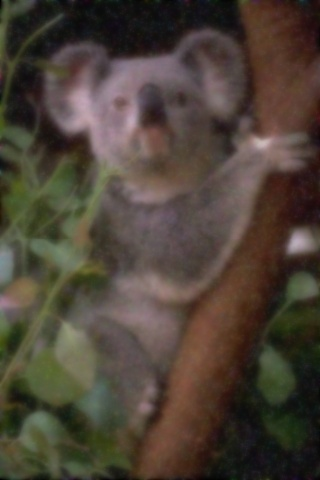
\includegraphics[scale=0.38]{figures/chapter2/denoising/coala-tikhonov.png}
}%
\subfloat[Total Variation]{
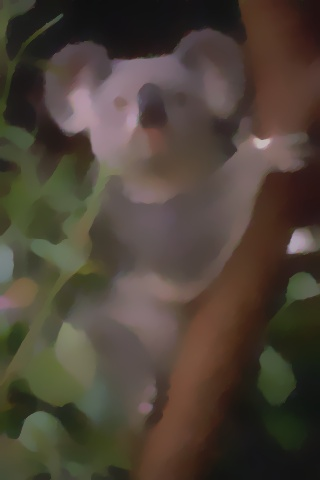
\includegraphics[scale=0.38]{figures/chapter2/denoising/coala-chambolle.png}
}%
\caption{Denoising algorithms results for the Tikhonov and Total variation regulararization terms.}
\label{ch1:fig:denoising-results}
\end{figure}



\section{Solving by a discrete strategy}
	\subsection{MRF and Gibbs distribution equivalence}
	\subsection{Potts model}
	\subsection{Graph-cuts}

\section{Digital approach}

%There is an equivalence between Gibbs distributions and MRF.
%
%Maximum a posteriori is also called penalized maximum likelihood
%
%Consider the problem to find $x$ such that $Ax=b$. If the problem has none or several solutions, the problem is said do be ill-posed. The standard method to solve it is by least-squares plus a penalty term. $|Ax-b|^2 + \lambda P$. The term $P$ models a preference for solutions with some desirable property, e.g., $P=|x|^2$ will favor solutions with lower norm.
%
%Tikhonov regularization is a type of L2 regularization. It is known to improve the problem conditioning and to enable direct solutions (wikipedia article).
	\chapter{Curvature as regularization}
\label{chapter:curvature-prior}

The curvature is a geometric property of curves and it measures the rate of change in curve orientation. A straight line has zero curvature while the curvature at corner of a square is infinity. The curvature is measured with respect to the arc-length parametrization, and it is invariant to translations, rotations and reflections (rigid transformations).

In imaging, the most widely use of curvature is, perhaps, as a smooth regularization term. That was the case in the Geometric Active Contour and Chan-Vese image segmentation models of~\cref{chapter:variational-methods-in-image-processing}. The curvature action in these models is closed related with the \emph{curve-shortening flow} applied to the image level curves. Additionally, the curvature also appears in the derivation of the TV denoising model.

Beyond the smoothing role, curvature can be used to favor connectivity, suggesting that its use could be valuable in the segmentation of thin and elongated objects, a difficult class to standard segmentation models. In image inpainting, the \emph{elastica curve} revealed to be a suitable model to mimic the amodal completion phenomenon, believed to be the process behind the human vision in the perception of occluded objects. However, elastica minimization is a challenging task, mainly because of its non-convexity and the $4th$ order expression emerging from its Euler-Lagrange equation.

In~\cref{ch3:sec:curvature-curve-shortening-flow,ch3:sec:diffusion-level-curves-motion}, we recall the definition of curvature and point out its role in some earlier imaging models. In~\cref{ch3:sec:elastica-curve} we describe the elastica curve, and the challenges involved in the minimization of the elastica energy. We dedicate~\cref{ch3:sec:discrete-methods-squared-curvature} to describe discrete models aiming the minimization of the elastica energy, which is an important topic of this thesis.



\section{Curvature and the curve-shortening flow}
\label{ch3:sec:curvature-curve-shortening-flow}

The curvature is a fundamental geometric property of curves and it widely present in geometric imaging models. In this section we start by recalling the curvature definition and some of its mathematical representations. Next we describe the \emph{curve-shortening flow} for planar curves, the one dimensional case of the mean curvature flow.

\subsubsection{Definitions}
In the remain of this section, we assume that every curve is regular, planar and counter-clockwise oriented. Let $C:[0,L(C)]\rightarrow \mathbb{R}^2$ a curve parameterized by arc-length, i.e.,
\begin{align*}
	C(s) &= (x(s),y(s)).
\end{align*}
%
Let $T(s)$ and $N(s)$ two orthonormal vectors to $C(s)$, i.e., the unitary tangent and normal to $C(s)$. Writing $C(s)$ using these orthonormal vectors we obtain
\begin{align*}
	C(s) &= \left( C(s) \cdot T(s) \right)T(s) + \left( C(s) \cdot N(s) \right)N(s)
\end{align*}
%
Notice that $\frac{\partial C}{\partial s} = T(s)$, therefore
\begin{align*}
	\frac{\partial C}{\partial s} \cdot \frac{\partial C}{\partial s} = \bignorm{ \frac{ \partial C}{\partial s} }^2 = 1.
\end{align*}
%
Derivating the last expression in both sides we obtain
\begin{align*}
	0 &= 2\frac{\partial ^2 C}{\partial s} \cdot \frac{\partial C}{\partial s} \\
	  &= 2\frac{\partial ^2 C}{\partial s} \cdot T(s).
\end{align*}
%
We conclude that $\frac{\partial ^2 C}{\partial s}$ is orthogonal to $T(s)$, and that the curvature is given by the normal component of $\frac{\partial ^2 C}{\partial s}$, i.e.,
\begin{align*}
	\frac{\partial ^2 C}{\partial s} &= \kappa(s) N(s).
\end{align*}
%
We have several formulations for curvature, some of them listed below (for a full derivation see the appendix). 
\begin{align*}
\begin{array}{rrl}
	\textbf{Arc-length parameterization:} & \displaystyle \kappa(s) &= \displaystyle \bignorm{ \frac{\partial^2 C}{\partial s^2} }. \\[1.5em]	
	\textbf{Arbitrary parameterization:} & \displaystyle \kappa(u) &= \displaystyle \frac{y'x'' - x'y''}{\left( x'^2 + y'^2 \right)^{3/2}}. \\[1.5em]
	\textbf{Implicit function:} & \displaystyle \kappa(x,y) &= \displaystyle -\frac{f_{xx}^2 - 2f_xf_yf_{xy} + f_{yy}^2}{\norm{\nabla f}^3} \\[1.5em]
	&&= \displaystyle \nabla \cdot \left( \frac{\nabla f}{\norm{\nabla f}} \right).
\end{array}
\end{align*}
%
%

\subsubsection{Curve-shortening flow}
\label{ch3:sec:curve-shortening-flow}

Let $ t\geq 0$ and $u \in [0,U]$, for some $U>0$. Next, let the $C^{(0)}:[0,U] \rightarrow \mathbb{R}^2$ and $\mathcal{C}(t,u)$ a family of curves such that
\begin{align}
	\mathcal{C}(0,u) & = C^{(0)}(u) \\
	\frac{\partial \mathcal{C}}{\partial t}(t,u) &= v(t,u) N(t,u),
	\label{ch3:eq:curve-normal-flow}
\end{align}
%
where $v$ is an arbitrary smooth function. The curve ${C}^{(t)}$ is deformed at each point $p$ by an amount $v$ in the normal direction at $p$. Note that any tangent component is irrelevant to curve deformation. From~\cref{ch3:eq:curve-flow} we compute the first variation of curve length of family $\mathcal{C}$
\begin{align*}
	\frac{\partial }{\partial t}L(t) &= \frac{\partial}{\partial t}\int_{0}^{U}{\norm{ \mathcal{C}_u } du} \\
	&= \int_{0}^{U}{ \frac{ \mathcal{C}_u \cdot \mathcal{C}_{ut} }{\norm{\mathcal{C}_u} } du} \\
	&= \int_{0}^{U}{ T \cdot \left( \mathcal{C}_{t} \right)_u  du}.
\end{align*}
%
Changing from an arbitrary parameterization $u$ to an arc-length one and recalling that $ds=\norm{ \mathcal{C}_u }  du$
\begin{align*}
	\frac{\partial }{\partial t}L(t) &= \int_{0}^{U}{ T \cdot \left( \mathcal{C}_{t} \right)_s \norm{ \mathcal{C}_u }  du} = \int_{0}^{L(\mathcal{C})}{ T \cdot \left( \mathcal{C}_{t} \right)_s ds}. 	
\end{align*}
%
Using~\cref{ch3:eq:curve-normal-flow} we obtain
\begin{align*}
	\frac{\partial }{\partial t}L(t) &= \int_{0}^{L(\mathcal{C})}{T \cdot (-\kappa vT + v_sN) ds } = - \int_{0}^{L(\mathcal{C})}{\kappa v ds} = -<\kappa,v>.
\end{align*}
%
From which we conclude that length decreases the fastest by choosing $v=\kappa$. We define the \emph{curve-shortening flow} (CS flow) of curve $C^{(0)}(u)$ as the family $\mathcal{C}(t,u)$ such that
\begin{align}
	\mathcal{C}(0,u) & = C^{(0)}(u) \\
	\frac{\partial \mathcal{C}}{\partial t}(t,u) &= \kappa(t,u) N(t,u).
	\label{ch3:eq:curve-shortening-flow}
\end{align}
%
%
\textbf{Example:} Let $C^{(0)}$ be a circle of radius $R_0$, i.e.,  $C^{(0)} = R_0( \cos t, \sin t)$. From~\cref{ch3:eq:curve-shortening-flow} we conclude that for every $t \geq 0$, $C^{(t)}$ is a circle of radius $R(t)$ where
\begin{align}
	\frac{\partial R}{\partial t} &= -\frac{1}{R}  \rightarrow R(t) = \sqrt{R_0^2 - 2t}.
	\label{ch3:eq:curvature-flow-circle}
\end{align}
%
Moreover, the curve collapses to a single point in time $t=\frac{R_0^2}{2}$. The curvature flow has many interesting properties~\cite{huisken84flow,gage86heat,ecker08heat}. Among them,

\begin{itemize}
	\item[]{\textbf{Comparison principle:} Let $C_1$,$C_2$ two closed curves such that $C_1^{(0)}$ is in the interior of $C_2^{(0)}$. Then $C_1^{(t)}$ is in the interior of $C_2^{(t)}$ for every $t$.}
	\item[]{\textbf{Convexity preserving:} A convex curve $C^{(0)}$ stays convex for all $t$.}
	\item[]{\textbf{Point collapsing:} Let $C^{(0)}$ a closed curve. There exists a time $t$ in which $C^{(t)}$ describes a circle and it follows~\cref{ch3:eq:curvature-flow-circle} until collapsing into a single point.}
	\item[]{\textbf{Perimeter minimization:} The curvature flow is the continuous deformation that decreases the perimeter of a single closed curve the fastest.}
\end{itemize}


The CS flow appeared in the Chan-Vese and Geometric Active Contour models for image segmentation in~\cref{chapter:variational-methods-in-image-processing} in its level set formulation~\cite{osher88fronts}
\begin{align}
	\frac{\partial f}{\partial t} &= \norm{\nabla f}\nabla \cdot \left( \frac{\nabla f}{\norm{\nabla f}} \right).
	\label{ch3:eq:implicit-curvature-flow}
\end{align}
%
In this case, each of the image level curves describes a CS flow.

\begin{figure}
\center
\subfloat[]{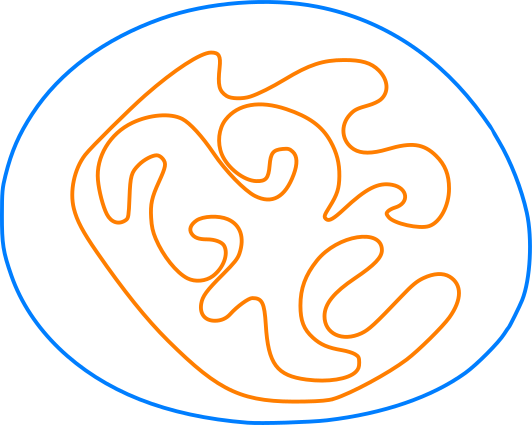
\includegraphics[scale=0.36]{figures/chapter3/curve-shortening-flow/1.png}}\hspace{1em}
\subfloat[]{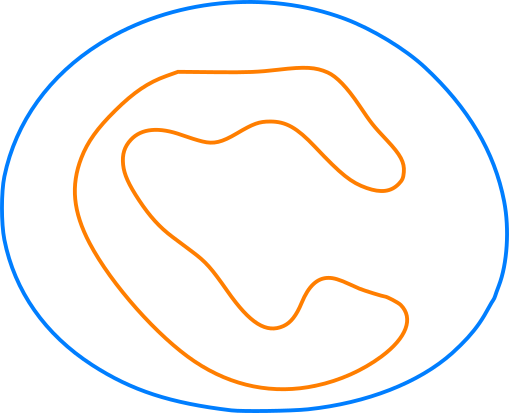
\includegraphics[scale=0.36]{figures/chapter3/curve-shortening-flow/2.png}}\hspace{1em}
\subfloat[]{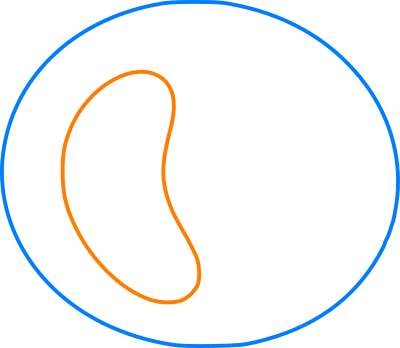
\includegraphics[scale=0.36]{figures/chapter3/curve-shortening-flow/3.png}}\hspace{1em}
\subfloat[]{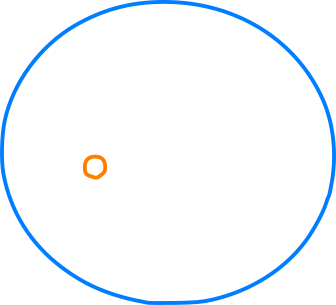
\includegraphics[scale=0.36]{figures/chapter3/curve-shortening-flow/4.png}}
\caption{\textbf{CS flow in action.} CS flow at different times in evolution. In this example we observe the CS flow properties listed in the text.}
\end{figure}



\section{Diffusion and level curves motion}
\label{ch3:sec:diffusion-level-curves-motion}

Several models in~\cref{chapter:variational-methods-in-image-processing} are stated as diffusion processes, but quite often a level curve evolution interpretation is more convenient. In this section we analyze the role of curvature, its properties in earlier models of image processing and how the dual interpretation of these models help us to gain extra insight on them.

\subsubsection{Curvature in denoising and image segmentation}

The necessary optimality condition of the total variation denoising energy is given by
\begin{align}
	\nabla \cdot \left( \frac{\nabla f}{\norm{\nabla f}} \right) + \lambda( f_{\widetilde{\vec{I}}} - f ) &= 0.
	\label{ch3:eq:total-variation-optimal-condition}
\end{align}
%
The solution of~\cref{ch3:eq:total-variation-optimal-condition} is the steady state of the  anisotropic diffusion
\begin{align}
	u(0,x) &= f(x) 	\label{ch3:eq:tv-flow-1} \\
	\frac{\partial u}{\partial t} &= \nabla \cdot \left( \frac{\nabla f}{\norm{\nabla f}} \right) + \lambda( f_{\widetilde{\vec{I}}} - f ). \label{ch3:eq:tv-flow-2}
\end{align}
%
Note the similarity between~\cref{ch3:eq:tv-flow-2} and the level set formulation of the CS flow in~\cref{ch3:eq:implicit-curvature-flow}. If $\lambda=0$, we denote~\cref{ch3:eq:tv-flow-1,ch3:eq:tv-flow-2} the \emph{TV flow}\cite{bellettini02total}. Interestingly, both CS flow and TV flow decrease total variation of $f$, but in different ways. The CS flow tends to deform the boundary of objects and decreasing total variation by perimeter minimization. The TV flow, on the other hand, preserves the boundary for longer and it decreases the TV by decreasing the surface height, i.e., the color intensity of the pixels(see~\cref{ch3:fig:minimization-tv-curvature-tv-flow}).

Naturally, the CS flow can also be used to do image denoising. If we think of noise as small artifacts with high gradient of color, the level curves corresponding to noise will have a very small radius, and will collapse faster than other level curves (see~\cref{ch3:fig:denoising-tv-curvature}). 


In the geometric active contours model for image segmentation, the level sets of a predefined function $u$ (e.g., a smoothed version of function $1-\lambda_C$ where $C$ is a set that contains the object to be segmented) describes a CS flow motion modulated by an edge detector function $g$ (e.g., $g=(1+\norm{ \nabla f })^{-1}$).
\begin{align*}
	u(0,x,y) &= u(x,y) \nonumber \\
	\frac{du}{dt} &= g( \norm{\nabla f} )\norm{\nabla u}\nabla \cdot \left( \frac{\nabla u}{\norm{\nabla u}}  + v \right),
\end{align*}
%%
%
%
\begin{figure}
\center
	\subfloat{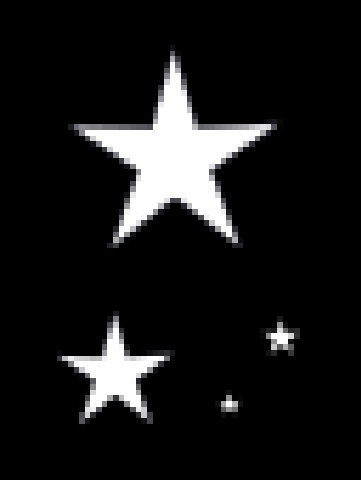
\includegraphics[scale=0.15,valign=t]{figures/chapter3/tv-curvature-stars/curvature/stars.png}}\hspace{0.2em}
	\begin{tabular}[t]{m{0.25cm}cc|cc}
	& \multicolumn{2}{c|}{$\norm{\nabla f_I}=25$} & \multicolumn{2}{c}{$\norm{\nabla f_I}=15$} \\
	\hline
	\rotatebox{90}{CS flow} & \figTable{0.2}{figures/chapter3/tv-curvature-stars/curvature/stars-25.png} & \figTable{0.2}{figures/chapter3/tv-curvature-stars/curvature/levels-stars-25.png} & \figTable{0.2}{figures/chapter3/tv-curvature-stars/curvature/stars-15.png} & \figTable{0.2}{figures/chapter3/tv-curvature-stars/curvature/levels-stars-15.png} \\
	\rotatebox{90}{TV flow} & \figTable{0.2}{figures/chapter3/tv-curvature-stars/tv/stars-25.png} & \figTable{0.2}{figures/chapter3/tv-curvature-stars/tv/levels-stars-25.png} & \figTable{0.2}{figures/chapter3/tv-curvature-stars/tv/stars-15.png} & \figTable{0.2}{figures/chapter3/tv-curvature-stars/tv/levels-stars-15.png}
	\end{tabular}
	\caption{\textbf{Minimizing TV energy with TV flow and CS flow.}Both flows decrease the image total variation, but CS flow tends to deform object boundaries while doing so. On the other hand, TV flow reduces the image contrast.}
	\label{ch3:fig:minimization-tv-curvature-tv-flow}	
\end{figure}
%
\begin{figure}
\center
\subfloat{\includegraphics[scale=0.224,valign=t]{figures/chapter3/tv-curvature-coala/curvature/coala-original.png}}\hspace{0.2em}\setcounter{subfigure}{0}
\subfloat[Noisy Image]{\includegraphics[scale=0.32,valign=t]{figures/chapter3/tv-curvature-coala/curvature/coala-noise.png}}\hspace{1em}
\subfloat[CS flow]{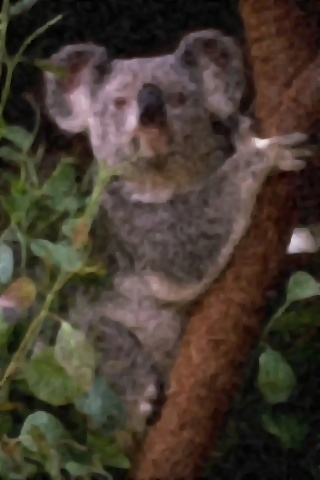
\includegraphics[scale=0.32,valign=t]{figures/chapter3/tv-curvature-coala/curvature/coala-30.png}}\hspace{1em}
\subfloat[TV flow]{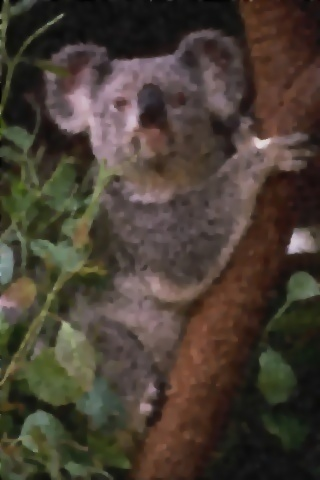
\includegraphics[scale=0.32,valign=t]{figures/chapter3/tv-curvature-coala/tv/coala-30.png}}
\caption{\textbf{TV denoising using CS and TV flow.}Results are quite similar, but TV flow image is sharper, although with lower contrast than CS flow. Images (b) and (c) have the same TV value.}
\label{ch3:fig:denoising-tv-curvature}
\end{figure}
%
\subsubsection{Curvature and the connectivity principle applied to inpainting}

We recall that the inpainting problem consists into reconstructing a collection of missing patches $\mathcal{P}$ of the image. The earlier inpainting model~\cite{bertalmio00image}  diffuses image information through the patches boundaries. The particularity of this model is that the Laplacian (heat equation) is diffused along the image level lines. Besides its impressive results, this models does not possess an important property which is expected in inpainting models: the \emph{connectivity principle}.


\begin{figure}
\center
\subfloat[Amodal completion.\label{ch3:fig:amodal-completion}]{
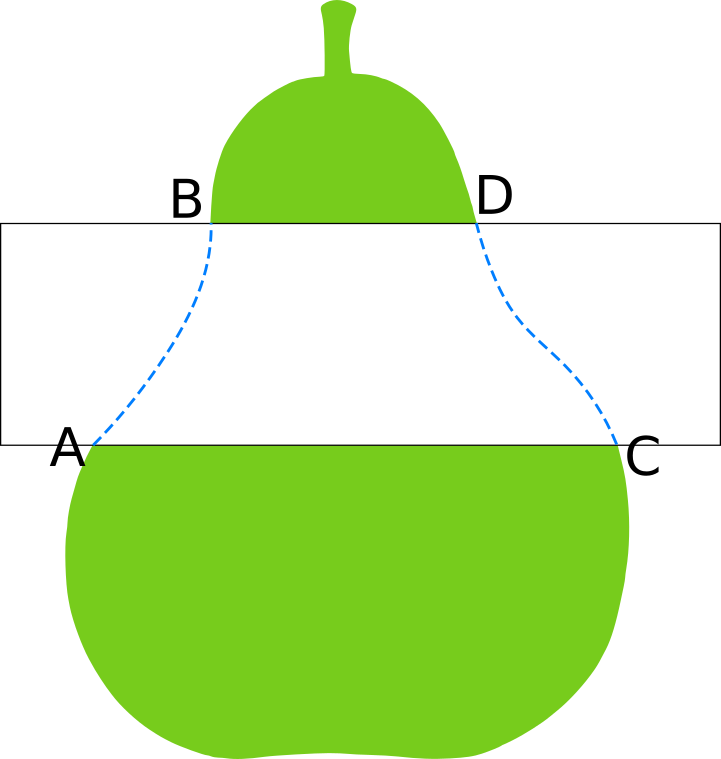
\includegraphics[scale=0.36]{figures/chapter3/amodal-completion.png}
}\hspace{3em}
\subfloat[Thin and elongated object segmentation.\label{ch3:fig:connectivity-principle}]{
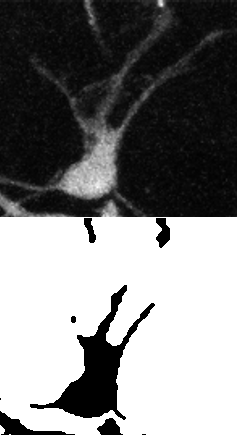
\includegraphics[scale=0.45]{figures/chapter3/vessels-bad-seg.png}
}
\caption{\textbf{Connectivity principle.} In~\cref{ch3:fig:amodal-completion}, an illustration of amodal completion, the process followed by the human vision to complete the boundary of occluded object with curves of low curvature ant that conform the most with the direction of the endpoints. In~\cref{ch3:fig:connectivity-principle} a vessel segmentation with length penalization term only. Curvature favors connected objects.}
\end{figure}

Studies of the Gestalt school of psychology suggest that the human vision, by a process called amodal completion~\cite{mumford94elastica}, completes the boundary of partially occluded object with a short and low curvature curve, as illustrated in~\cref{ch3:fig:amodal-completion}. The model proposed in~\cite{chan01nontexture} is a TV flow modulated by the curvature of the image level curves. 
\begin{align}
	u(0,x,y) &= f(x,y) \nonumber \\
	\frac{\partial u}{\partial t} &= \nabla \cdot \left( |\kappa(t)|\frac{\nabla f}{\norm{f}} \right) .
	\label{ch3:eq:inpainting-curvature-driven-diffusion}
\end{align}
%
The diffusion in~\cref{ch3:eq:inpainting-curvature-driven-diffusion} is stronger at points of high curvature with respect to its level curves. This model partially achieves the connectivity principle (see~\cref{ch3:fig:inpainting-curvature-driven-diffusion}), but the completion is done only for very small regions. 

The connectivity principle suggests that the curve connecting the endpoints of an occluded object should minimize some energy with respect the curvature. Moreover, the segmentation of thin and elongated objects may also benefit from a curvature term, since classical methods have difficulties to give connected solutions. In the next section we describe the Elastica, the curve that minimizes the squared curvature along its length.

\begin{figure}
\center

\includegraphics[scale=1]{figures/chapter3/inpainting-cdd/lake-1.png}\hspace{0.5em}
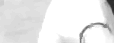
\includegraphics[scale=1]{figures/chapter3/inpainting-cdd/lake-2.png}\hspace{3em}
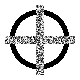
\includegraphics[scale=0.6]{figures/chapter3/inpainting-cdd/circle-1.png}\hspace{0.5em}
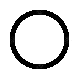
\includegraphics[scale=0.6]{figures/chapter3/inpainting-cdd/circle-2.png}
\caption{\textbf{Inpainting by curvature driven diffusions.}\cite{chan01nontexture} The diffusion process modeled by~\cref{ch3:eq:inpainting-curvature-driven-diffusion} completes the features disconnected by the inpainting mask.}
\label{ch3:fig:inpainting-curvature-driven-diffusion}
\end{figure}



\section{Elastica curve}
\label{ch3:sec:elastica-curve}

In 1691 James Bernoulli pose a challenge to your colleagues: What is the form taken by an elastic beam whose its endpoint $A$ is kept fixed in the ground while a weight is attached to its other endpoint $B$ such that the tangent at each of the endpoints are perpendicular? A simplified scheme is presented in~\cref{ch3:fig:james-scheme-elastica}.

\begin{figure}
\center
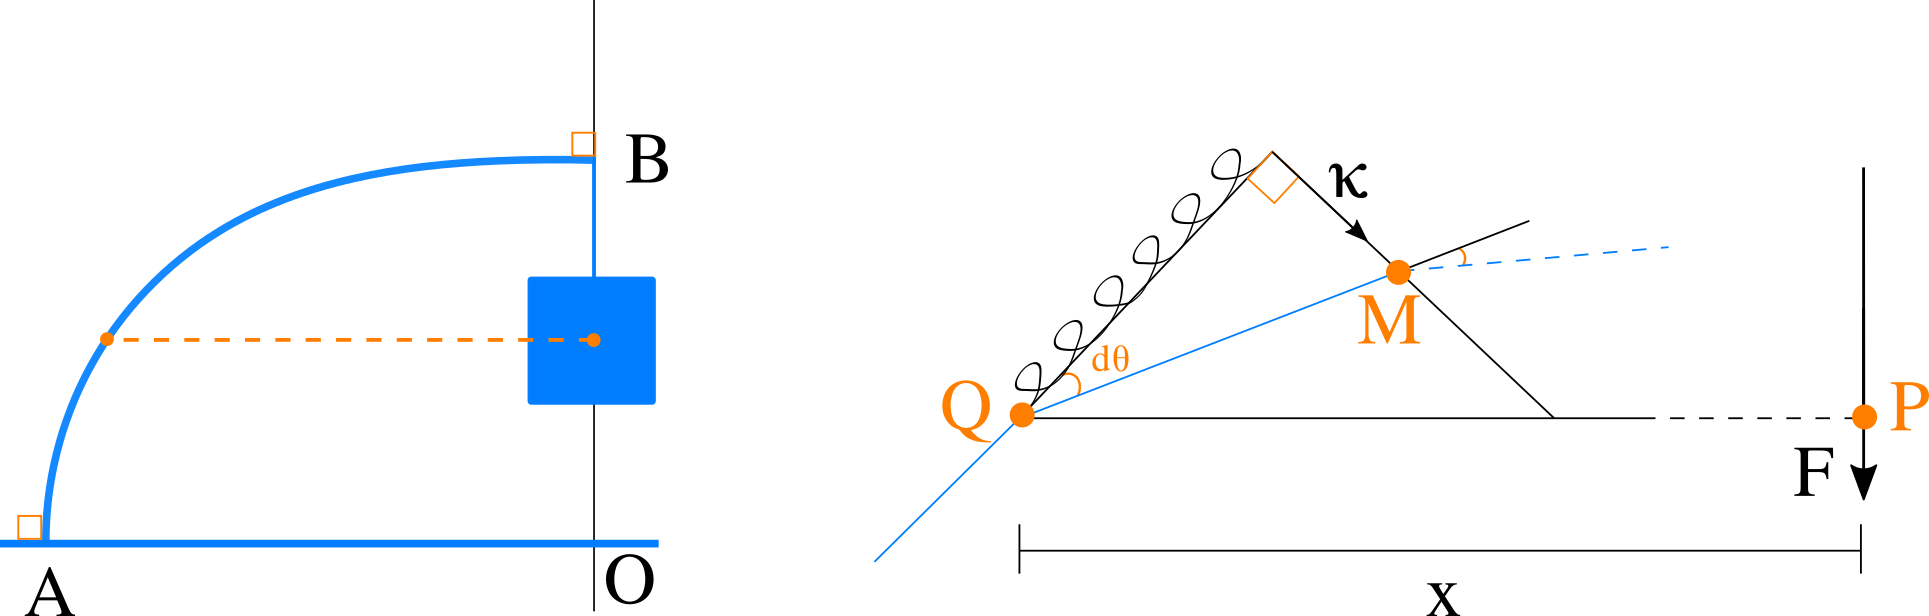
\includegraphics[scale=0.36]{figures/chapter3/elastica/james-scheme.png}
\caption{\textbf{Elastic beam and James Bernoulli's solution.} In equilibrium, the moments at the two ends of the virtual lever $PQM$ should cancel, implying that the curvature is a linear function of $x$ if we assume the spring behaves in accordance with Hooke's law.}
\label{ch3:fig:james-scheme-elastica}
\end{figure}

By using mechanical principles, James concluded that the curvature of such curve at some point $Q$ can be written as a linear function of the distance from $Q$ to the line $BO$, i.e., $\kappa(x) = cx$. One can show that~\cite{levien08elastica,truesdell60rational},
\begin{align}
	\frac{\partial y}{\partial x} &= \frac{cx^2}{ \sqrt{1-c^2x^4} }.
	\label{ch3:eq:rectangular-elastica}
\end{align}
%
The curve modeled by~\cref{ch3:eq:rectangular-elastica} is called the \emph{rectangular elastica}. The expression in the right cannot be integrated using elementary functions and is a member of the class of elliptic integrals. Fortunately, Euler has shown that one can express not only the rectangular elastica, but its general version in the form of a minimization principle. 

The generalized elastica in $2$D is the planar curve $C$ of fixed length $L$ whose endpoints have known tangents $C'(0)=\theta_0,C'(L)=\theta_L$ and minimizes the energy $\int_{C} \kappa^2 ds$.
\begin{align*}
	\begin{array}{rl}
		\displaystyle \min_{C} \int_{C}{\kappa ^2} \\[1em]
		\text{subject to}& \norm{C} = L,\\
		& C'(0) = \theta_0, \\
		& C'(L) = \theta_L.
	\end{array}	
\end{align*}
%
Given parameters $\alpha \geq 0, \beta \geq 0$ we incorporate the isoperimetric constraint in the objective function (can be interpreted as a Lagrange multiplier) to define the Elastica energy as
\begin{align}
	E(C) &= \int_{C}{\alpha + \beta \kappa^2 ds}.
	\label{ch3:eq:elastica-energy}
\end{align}
%
If we do not impose any constraint in~\cref{ch3:eq:elastica-energy}, its minimization is interesting only if $\alpha >0$ and $\beta >0$ and we call this problem the \emph{free Elastica}. On the other hand, if one imposes constraints to the minimization of~\cref{ch3:eq:elastica-energy}(e.g., fixed tangent endpoints), we refer to this problem as the \emph{unconstrained Elastica}.

One can easily derive the solution of the free Elastica for a closed curve. Setting $\beta=0$, the minimization of~\cref{ch3:eq:elastica-energy} behaves as the curve-shortening flow of section~\cref{ch3:sec:curve-shortening-flow}. On the other hand, if we set $\alpha =0$, the minimum is a disk of infinite radius. For the intermediate case, with both parameters greater than zero, it is easy to see that the solution is a circle $C_r$ of some radius $r$, therefore
\begin{align*}
	C_r = \argmin_C E(C) \rightarrow \frac{ \partial}{\partial r} \int_{C_r}{\alpha + \beta \kappa^2 ds} &= 0 \\
	\frac{\partial}{\partial r} \big( \alpha 2\pi r + \beta \pi/r \big) & = 0 \\
	r &= \left(\frac{\beta}{\alpha}\right)^{1/2}.
\end{align*}
%
In general, a planar curve $C$ minimizing the Elastica energy satisfies the following Euler-Lagrange equation~\cite{chan02elasticainpainting,singer08lectures}
\begin{align}
		2\kappa_{ss} + \kappa^3 = \frac{\alpha}{\beta}\kappa \Leftrightarrow \frac{\partial ^4 C}{\partial s^4} + \frac{\partial ^2 C}{\partial s^2}^3 = \frac{\alpha}{\beta}\frac{\partial ^2 C}{\partial s^2}.
		\label{ch3:eq:euler-lagrange-equation-elastica}
\end{align}
%
%
This fourth order expression is the main difficult in minimizing the Elastica. In the following we are going to describe some models that attempt to minimize the Elastica and the strategies employed.

\subsubsection{Imaging models using the Elastica}

In~\cite{chan02elasticainpainting} the authors propose an inpainting model in which the image level lines interrupted by the inpainting domain are completed by Elastica curves. The key is to define an energy that minimize each of the level curves in terms of the Elastica simultaneously. Given an image $f_I:\Omega \rightarrow [0,1]$, let $\Gamma_{\lambda}$ be one of its level curve, i.e.,
\begin{align*}
	\Gamma_{\lambda} &= \left\{ x \; | \; f_I(x)=\lambda \right\}.
\end{align*}
%
Therefore, we minimize each level curve in terms of the Elastica energy by minimizing the functional
\begin{align}
	\int_{0}^{1}{ \int_{\Gamma_{\lambda}}{ \left( \alpha + \beta \kappa ^2 \right) dsd\lambda}} = \int_{0}^{1}{ \int_{\Gamma_{\lambda}}{ \left(\alpha + \beta \nabla \cdot \left(\frac{\nabla f_I}{\norm{\nabla f_I}}\right) ^2 \right) dsd\lambda}}
	\label{ch3:eq:elastica-all-level-curves}
\end{align}
%
Next, let $dt$ be the length element in the normal direction of the level curves. Therefore,
\begin{align*}
	\frac{d \lambda}{d t} &= \norm{\nabla f_I} \rightarrow d\lambda = \norm{\nabla f_I}dt.
\end{align*}
%
Replacing the last expression in~\cref{ch3:eq:elastica-all-level-curves} we obtain
\begin{align}
	\int_{0}^{1}{ \int_{\Gamma_{\lambda}}{ \left(\alpha + \beta \nabla \cdot \left(\frac{\nabla f_I}{\norm{\nabla f_I}}\right) ^2 \right)\norm{\nabla f_I} dsdt}} &= \int_{\Omega}{ \left(\alpha + \beta \nabla \cdot \left(\frac{\nabla f_I}{\norm{\nabla f_I}}\right) ^2 \right)\norm{\nabla f_I}d\Omega}.
	\label{ch3:eq:chan-elastica-inpainting}
\end{align}
%
The last expression is derived from the fact that $dt$ and $ds$ are orthogonal length elements. The authors propose a finite difference scheme for the gradient flow derived from the Euler-Lagrange of~\cref{ch3:eq:chan-elastica-inpainting}, which happens to be of $4th$ order. The high order poses some issues with numerical instability, namely the definition of the time step and convergence analysis, which is skipped. The running time is also quite high even for small inpainting domains. Moreover, one can expect a local solution at most, and giving the highly non-convex character of the equation, an acceptable local solution might be very difficult to be found without a conveniently chosen initial solution. Finally, the  method tends to produce blurry edges even for small inpainting domains. 

The numerical instability arising from~\cref{ch3:eq:chan-elastica-inpainting} is lessen by the $3rd$ order gradient flow proposed in~\cite{ballester01filling}. The idea is to create a new variable $\theta$ to replace the unstable term $\nabla f_I / \norm{\nabla f_I}$ and include a penalization term that forces $\theta$ to assume the value of its original interpretation. The energy to be minimized is closely related to~\cref{ch3:eq:chan-elastica-inpainting} and is written as
\begin{align}
	\int_{\Omega}{a|\nabla \cdot \theta|^2\left(\alpha + \beta \norm{ k * f_I}\right)d\Omega} + \int_{\Omega}{ \norm{\nabla f_I} - \theta \cdot \nabla f_I d_{\Omega}},\quad \norm{\theta} \leq 1.
	\label{ch3:eq:ballester-inpainting}
\end{align}
%
The kernel $k$ (e.g. Gaussian) smooths image $f_I$ and is included due to numerical reasons. Nonetheless,~\cref{ch3:eq:ballester-inpainting} suffers from similar issues to those of~\cref{ch3:eq:chan-elastica-inpainting}. Generally, PDE-based methods encounter difficulties in producing solutions with discontinuities, one of the main features of images.

A discrete approach to inpainting is proposed in~\cite{masnou98inpainting}. The model's first step is to identify pairs of admissible T-junctions, i.e., pixels in the outer boundary of the inpainting domain that have the same color value and orientation (see~\cref{ch3:fig:masnou-tjunctions}). Due to a property of level curves, for every value color value $\lambda$ there is an even number of T-junctions. Next, let $J$ be the set of T-junctions and $\Gamma_j^t$ a curve connecting an admissible pair $(j,t)$. Additionaly, we denote $\theta_j,\theta_t$ the respective angles the curve $\Gamma_j^t$ makes with the associated level set at $j$ and $t$. The authors propose to find a matching $\mathcal{M}=\{ (j,t) \; | \; j,t\text{ admissible} \}$ and its respective curves such that it minimizes the energy

\begin{figure}
\center
\subfloat[T-junctions illustration~\cite{ambrosio03direct}\label{ch3:fig:masnou-tjunctions}]{
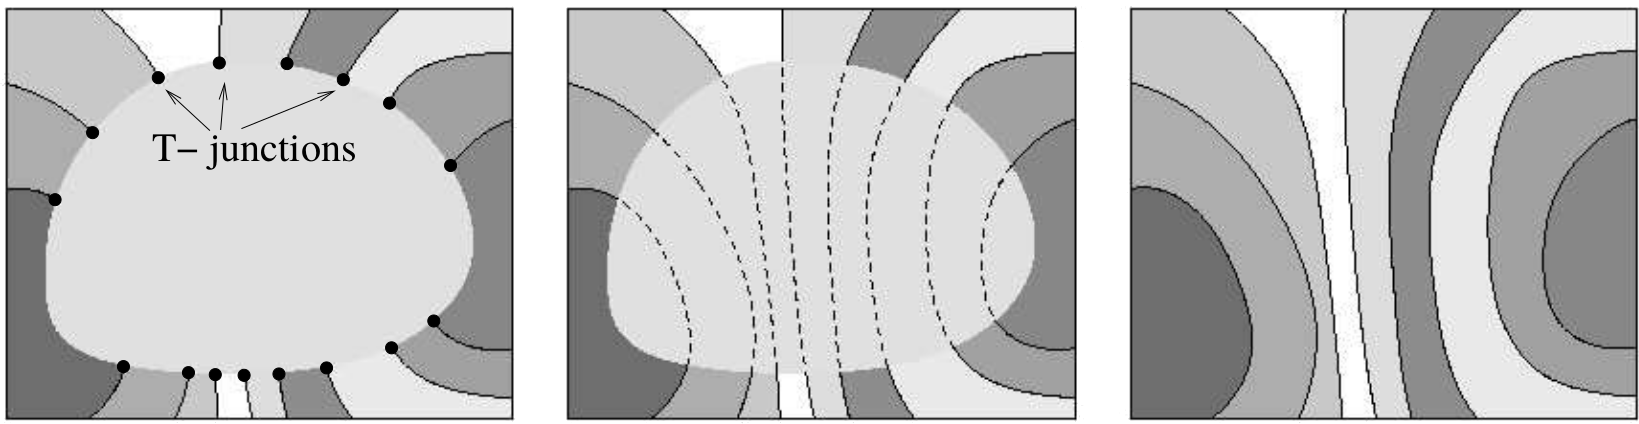
\includegraphics[scale=0.25]{figures/chapter3/masnou/tjunctions.png}}

\subfloat[Inpainting by~\cite{masnou98inpainting}\label{ch3:fig:masnou-inpainting}]{
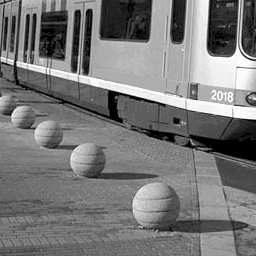
\includegraphics[scale=0.5]{figures/chapter3/masnou/tram-1.png}
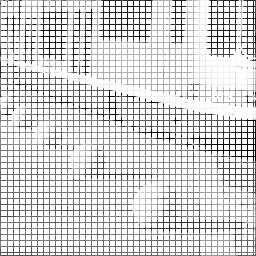
\includegraphics[scale=0.5]{figures/chapter3/masnou/tram-2.png}
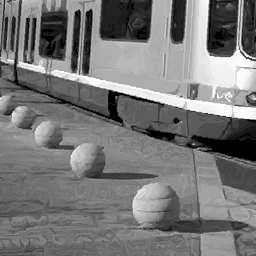
\includegraphics[scale=0.5]{figures/chapter3/masnou/tram-3.png}
}
\caption{\textbf{Discrete inpainting.} In~\cref{ch3:fig:masnou-tjunctions} an illustration of T-junctions and an ideal completion of the level lines; in~\cref{ch3:fig:masnou-inpainting} we have the original image in the left, the image to be inpainted in the middle and the result of the discrete inpainting in the right. }
\end{figure}
\begin{align}
	\sum_{(j,t) \in \mathcal{M}}{ \int_{\Gamma_j^t}{\alpha + \beta |\kappa|ds} + \theta_j + \theta_t }.
	\label{ch3:eq:masnou-inpainting}
\end{align}
%
%
Assuming that one knows the optimal matching $\mathcal{M}$, the curves connecting the T-junctions pairs are geodesics. In the plane, that means that the T-junctions are connected by polygonal curves. An ingenious dynamic programming algorithm is conceived  by exploiting the causality relation imposed by the non-crossing constraint of the level curves and excellent results are obtained. In particular, the algorithm can reconstruct large inpainting domains and does not produce blurry edges (see~\cref{ch3:fig:masnou-inpainting}). However,~\cref{ch3:eq:masnou-inpainting} cannot produce curvy level lines.


The work of~\cite{masnou98inpainting} illustrates an advantage of discrete approaches to image models: discontinuities are naturally implemented. To find a discrete model is not a trivial task, and sometimes a compromise needs to be done in order to achieve efficiency, as it was the case in~\cite{masnou98inpainting}, in which the absolute value of the curvature is used instead of its square. In the next section we are going to describe some discrete models for Elastica in its most known form, i.e., using the square of the curvature.


\section{Discrete methods and squared curvature}
\label{ch3:sec:discrete-methods-squared-curvature}

\subsubsection{Discrete elastica}

Let $\mathcal{P}_n=\{p_i \; | \; 1 \leq i \leq n\}$ a sequence of $n$ points describing a polygonal line. We define the following elements (an illustration is given in~\cref{ch3:fig:bruckstein-polygonal-line}).
\begin{align*}
\begin{array}{rll}
\text{Segment length:} & \quad \ell_i,& \quad 1 \leq i \leq n\\[0.5em]
\text{Segment angle:} & \quad \psi_i,& \quad 1 \leq i \leq n-1\\[0.5em]
\text{Angle deviation:} & \quad \theta_i,& \quad 1 \leq i \leq n-2.
\end{array}
\end{align*}
%
\begin{figure}
\center
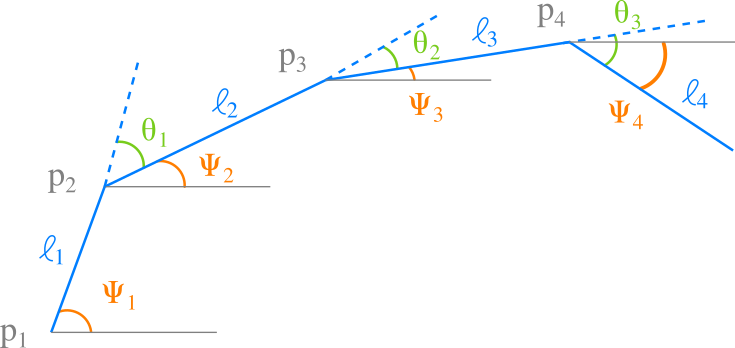
\includegraphics[scale=0.6]{figures/chapter3/bruckstein/polygonal-line.png}
\caption{\textbf{Discrete elastica.} The curvature is approximated by $\theta_i/l_i$.}
\label{ch3:fig:bruckstein-polygonal-line}
\end{figure}

Given parameters $\alpha \geq 0,\beta \geq 0$ and a fixed length segment $\ell$, the discrete elastica~\cite{bruckstein01discrete} is defined as
\begin{align}
	E(\vec{\theta},\ell) &= \ell \cdot \sum_{1 \leq i \leq n-2}{ \alpha + \beta \left(\frac{\theta_i}{\ell}\right)^2} = \sum_{1 \leq i \leq n-2}{ \alpha \ell + \beta \frac{\theta_i^2}{\ell}}.
	\label{ch3:eq:discrete-elastica}
\end{align}
%
Without loss of generality, we assume that the curve starts at the origin with tangent $\psi_1=t_1$ and ends at point $(L,0)$ with tangent $\psi_{n-1}=t_{n-1}$, $L$ being the curve length. Then, the general discrete elastica problem is defined as
\begin{align*}
	\min_{\vec{\psi},\ell}{ \sum_{1 \leq i \leq n-2 }{ \alpha \ell + \beta \frac{ (\psi_{i+1} - \psi_{i} )^2}{\ell}}}\\
	\begin{array}{rrl}
		\text{subject to}&& \\
		&\displaystyle \sum_{1 \leq i \leq n-1}{\ell\cos \psi_i} &= L, \\[1em]
		&\displaystyle \sum_{1 \leq i \leq n-1}{\ell\sin \psi_i} &= 0, \\[1em]
		&\displaystyle \psi_1 &= t_1, \\[1em]
		&\displaystyle \psi_{n-1} &= t_{n-1}.
	\end{array}
\end{align*}
%
The constraints can be included in the objective function with its respective Lagrange multipliers coefficients and we end up with a nonlinear system. In~\cite{bruckstein01discrete}, the authors reported that standard methods as Newton-Raphson return nice approximations of the continuous elastica. In a companion paper, the authors proved that a similar formulation of the discrete elastica, namely
\begin{align}
	E(\vec{\theta},l) &= \sum_{1 \leq i \leq n-2}{ \alpha \ell + \beta \left( \frac{\theta_i^2}{\min \left\{{\ell_i,\ell_{i+1}} \right\} }\right)}
	\label{ch3:eq:discrete-elastica}
\end{align}
%
is convergent in the sense of $\Gamma$-convergence~\cite{bruckstein01epi}, i.e., the minimizer of the discrete elastica approaches the minimizer of the elastica as the number of discretization points goes to infinity. 

The discrete elastica was proposed in the context of nonlinear splines with applications in shape design. In imaging, we have to consider additional constraints. For example,  digital images are defined in an uniform grid, while the discrete elastica imposes no restriction on the location of the interpolation points in the plane. In fact, this is a fundamental difference between discrete and digital settings. In the list that follows we point out some of the issues one has to handle in order to adapt the discrete elastica to be applied in image segmentation

\begin{enumerate}
	\item{\textbf{Data term:} The interpolation points should lie close to the contour of objects and by doing that we lose the implicit description of the curve as a sequence of lengths and angle deviations, being forced to also consider the points coordinates;}
	\item{\textbf{Contour complexity:} We are handling closed contours, meaning that we likely have to minimize not one but many elasticas along a single contour (not to mention multisegmentation). In practice, that means that we have to chose feature points in the image to force the curve to pass through them;}
	\item{\textbf{Point sampling:} Finally, one has to decide how many points to use in the interpolation and where to position them (a uniform sampling is unlikely a good strategy), bearing in mind the compromise between number of points and computation time.}
\end{enumerate}




\subsubsection{Linear programming model for image segmentation using the discrete elastica}

In~\cite{schoenemann09linear}, the authors handle the previous list of issues by considering only the discrete elasticas lying on a $2$D cellular complex. The $2$D cellular complex is composed by non-overlapping surfaces called \emph{cells} and its lower dimension components: \emph{linels} and \emph{pointels}. The cellular complext forms a tessellation of the plane and the shape of the cells is arbitrary. The chosen cellular complex has a direct influence in the quality of the discrete elastica, as a finer tessellation covers a larger range of angles (see~\cref{ch3:fig:schoenemann-connectivity-1,ch3:fig:schoenemann-connectivity-2}). To simplify exposition, we are going to describe the model for a standard cellular grid complex, in which each cell represents a single pixel in the image.

\begin{figure}
\center
%\subfloat[\label{ch3:fig:cell-complex-1}]{
%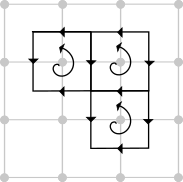
\includegraphics[scale=0.6]{figures/chapter3/schoenemann/schoenemann_cell_linel_orientation.png}
%}\hspace{0.5em}
%\subfloat[\label{ch3:fig:cell-complex-2}]{
%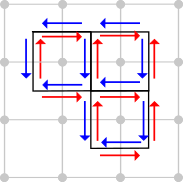
\includegraphics[scale=0.6]{figures/chapter3/schoenemann/schoenemann_oriented_edges.png}
%}\hspace{0.5em}
\subfloat[\label{ch3:fig:cell-complex-3}]{
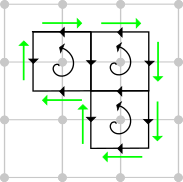
\includegraphics[scale=0.6]{figures/chapter3/schoenemann/valid_solution_0.png}
}\hspace{0.5em}
\subfloat[\label{ch3:fig:cell-complex-4}]{
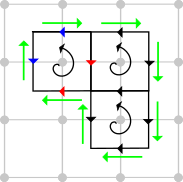
\includegraphics[scale=0.6]{figures/chapter3/schoenemann/valid_solution_1.png}
}\hspace{0.5em}
\subfloat[\label{ch3:fig:cell-complex-5}]{
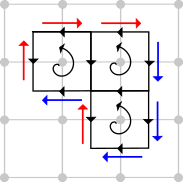
\includegraphics[scale=0.6]{figures/chapter3/schoenemann/valid_solution_2.png}
}
\caption{\textbf{Digital surface and consistency constraints.} In~\cref{ch3:fig:cell-complex-3}, a valid solution made of three cells and a sequence of eight linels. In~\cref{ch3:fig:cell-complex-4} the sum of linel-cell incidence equals to zero (blue are positively incident and red negatively incident). In~\cref{ch3:fig:cell-complex-5}, the sum of linel-edge incidence equals to zero.}
\label{ch3:fig:schoenemann-consistency-constraints}
\end{figure}

Let $n,m$ the number of cells and edges, respectively. We establish a convention on cells and linels orientation. We define the positive orientation of a cell as being counter-clockwise and the positive orientation of linels as being left (horizontal) and down (vertical), as indicated in the figure below. 

\begin{center}
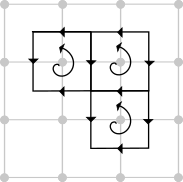
\includegraphics[scale=0.6]{figures/chapter3/schoenemann/schoenemann_cell_linel_orientation.png}
\end{center}

One binary variable is defined for each cell and two other binary variables are defined for each linel, one for each possible orientation the linel may assume. We refer to the variables associated to linels as edges. The variables are grouped in vector $\vec{x} \in \{0,1\}^{n+2m}$ and, hence, a solution is made of active cells and active edges. However, we have to make sure that solutions are consistent, i.e., a solution $\vec{x}$ must encode a digital surface. 

A digital surface is composed of a set of cells and a closed path (loop) of edges forming its boundary. To enforce digital surfaces, we define an incidence relation between linels and cells and between linels and edges. This relation is encoded by matrix $\vec{A} \in \{-1,0,1\}^{m\times(n+2m)}$ 
\begin{align*}
	\vec{A}_{i,j} &= \left\{ \begin{array}{rl}
		1,& \text{if positive incident}\\
		-1,& \text{if negative incident}\\
		0,& \text{otherwise}.		
	\end{array}\right.
\end{align*}
%
We say that a linel is positive incident to a cell if their orientations agree and negative incident if they disagree. Similarly, a linel is positive (negative) incident to an edge if they agree (disagree) in orientation. The space of solution is correctly restricted to digital surfaces by imposing
\begin{align*}
	\vec{A}\vec{x} &=0,
\end{align*}
%
i.e., the sum of incidences for each linel must equal to zero~(see~\cref{ch3:fig:schoenemann-consistency-constraints}). Finally, we set vector $\vec{w} \in \mathbb{R}^{n+2m}$ that is going to hold the data, length and squared curvature penalization terms. For example, data term coefficients are associated to cells variables while length and curvature terms are associated to edges. The complete formulation is written as
\begin{align*}
	\begin{array}{rl}
		\min_{\vec{x}} & \vec{w}^t\vec{x}\\
		\text{subject to} & \vec{A}\vec{x} = 0 \\
		& \vec{x} \in [0,1]^{n+2m},
	\end{array}
\end{align*}
%
%
where vector $\vec{x}$ was relaxed. The quality of the model naturally depends of the plane tessellation defined by the chosen cellular complex. A simple grid complex is not that interesting, as the discrete elastica can turn only on multiples of $\pi/2$. The authors present results for two different cellular complexes. They are equivalent to $8$-connectivity or $16$-connectivity in a graph-cut framework. 

The data term issue is handled by separating the roles of cells and edges. Cells variables holds data terms and edge variables hold curvature and length information. The refinement of the cellular complex is done via pixel subdivision, therefore, every cell lying in the interior of a pixel $p$ carries data term relative to pixel $p$. The consistency constraints guarantees well defined boundaries and the contour complexity issue is also covered. Finally, the model is extendable to different angular resolutions while keeping a digital setting, and a discrete elastica with an arbitrary sequence of interpolation points can be well approximated given a good choice of the cellular complex.

Some results are displayed in~\cref{ch3:fig:schoenemann-results}. However, the computation time is quite high and the segmentation present sharp angles even when employing a $16$-connectivity cellular complex.

\begin{figure}
\begin{minipage}{0.25\textwidth}
\center
\subfloat[\label{ch3:fig:schoenemann-connectivity-1}]{
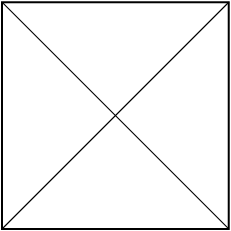
\includegraphics[scale=0.25]{figures/chapter3/schoenemann/neighborhood_system_8.png}
}

\subfloat[\label{ch3:fig:schoenemann-connectivity-2}]{
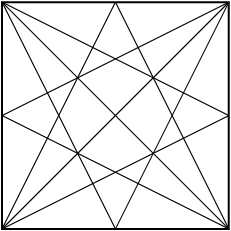
\includegraphics[scale=0.25]{figures/chapter3/schoenemann/neighborhood_system_16.png}
}
\end{minipage}%
\begin{minipage}{0.75\textwidth}
\center
\subfloat[\label{ch3:fig:schoenemann-results}]{
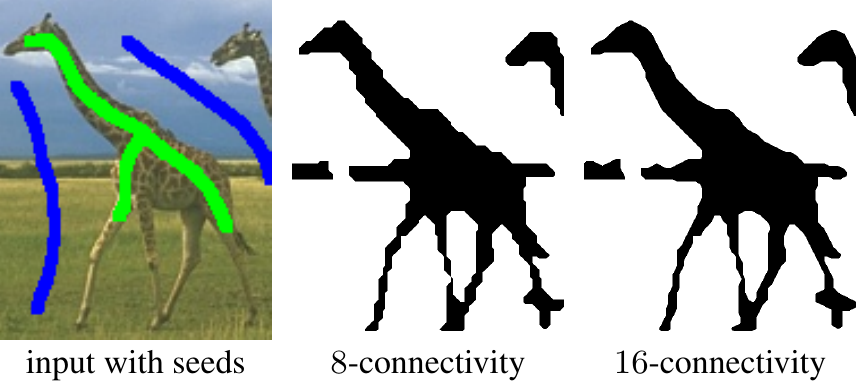
\includegraphics[scale=0.3]{figures/chapter3/schoenemann/schoenemann.png}
}
\end{minipage}%
\caption{\textbf{Linear programming model~\cite{schoenemann09linear}.} In the left, examples of the $8$ and $16$-connectivity cellular complexes. The authors implementation consists into subdivide a pixel. For example, the $8$-connectivity is implemented by rescaling the image twice its size and let the model unit being composed of $4$ pixels of the rescaled image. In the right, a result with different connectivities using a data term derived from given foreground (green) and background (blue) seeds. }
\end{figure}

\subsubsection{Unconstrained formulations}

The high number of variables and constraints explain the high running time of the linear programming approach. In~\cite{zehiry10fast}, the authors encode the squared curvature value in an unconstrained quadratic non-submodular PBF and propose a model for binary image segmentation.

Let $I$ be a digital image with $n$ pixels. We associate to each pixel the binary variable $\vec{x}_i$ indicating if the pixel belongs to foreground ($x_i=1$) or background ($x_i=0$). For a given segmentation $\vec{x}$, one can identify $90$ degrees turns in the segmentation contour by inspecting sequential pairs of vertices neighbors (given an order on the neighbors), as illustrated in figure~\cref{ch3:fig:elzehiry-turn-angles}. The turns can expressed as a $3$-clique potential, as shown in the table below

\begin{center}
\begin{tabular}{|c|c|c|c|}
\hline
$x_i$ & $x_j$ & $x_k$ & $w$ \\
\hline 
0 & 0 & 0 & 0 \\
0 & 0 & 1 & 0 \\
0 & 1 & 0 & 0 \\
0 & 1 & 1 & $w_{ijk}$ \\
1 & 0 & 0 & $w_{ijk}$ \\
1 & 0 & 1 & 0 \\
1 & 1 & 0 & 0 \\
1 & 1 & 1 & 0 \\
\hline 
\end{tabular}
\end{center}

\begin{figure}
\center
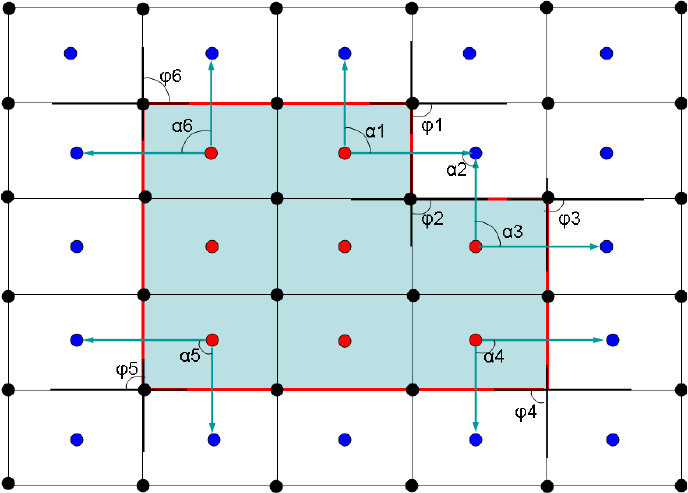
\includegraphics[scale=0.25]{figures/chapter3/elzehiry/turn-angles.png}
\caption{\textbf{Turn angles detection and triplets~\cite{zehiry10fast}.} Assuming that red pixels correspond to $1$-labeled variables and blue the $0$-labeled ones, angle variation is triggered by configurations $(x_i=1,x_j=0,x_k=0)$ and $(x_i=0,x_j=1,x_k=1)$, assuming that $x_i$ is the centered variable. }
\label{ch3:fig:elzehiry-turn-angles}
\end{figure}

The coefficients $w_{ijk}$ are defined accordingly with the Brucksteins discretization formula for the elastica, i.e.,
\begin{align*}
	w_{ijk} &= \frac{ \alpha_i ^2}{\min \{ |e_{ij}|,|e_{jk}| \} }.
\end{align*}
%
Remarkably, the $3$-clique potential can be decomposed in three $2$-cliques potentials 
\begin{align}
	E(x_i,x_j,x_k) &= w_{ij}(x_i-x_j)^2 + w_{ik}(x_i-x_k)^2 + w_{jk}(x_j-x_k)^2,
	\label{ch3:eq:elzehiry-pairwise}
\end{align}
%
where
\begin{align*}
	w_{ij} &= \frac{1}{2}w_{ijk} \\
	w_{ik} &= \frac{1}{2}w_{ijk} \\	
	w_{jk} &= -\frac{1}{2}w_{ijk}.
\end{align*}
%
~\cref{ch3:eq:elzehiry-pairwise} is a non-submodular PBF (the negative $w_jk$ coefficient creates a non-submodular term) and it is optimized using QPBO or one of its variations. The computation is much faster than the linear programming formulation and the model favors the connectivity principle, although the completion effect seems limited to very small portions~(see~\cref{ch3:fig:elzehiry-results}). A clear drawback is the limitation in the angle resolution, which tends to produce block artifacts. The authors argue that the model can be extended to any desired connectivity, but it is not clear how this is done.

\begin{figure}
\center
\begin{tabular}{ccc}
\subfloat[Original]{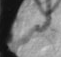
\includegraphics[scale=1.25]{figures/chapter3/elzehiry/vessel-1.png}} &
\subfloat[Data]{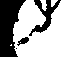
\includegraphics[scale=1.25]{figures/chapter3/elzehiry/vessel-2.png}} &
\subfloat[Data+Curvature]{\quad\quad 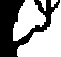
\includegraphics[scale=1.25]{figures/chapter3/elzehiry/vessel-3.png}\quad\quad} \\[1em]
\subfloat[Original]{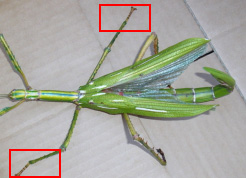
\includegraphics[scale=0.3]{figures/chapter3/elzehiry/insect-1.png}} &
\subfloat[Data]{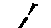
\includegraphics[scale=1.25]{figures/chapter3/elzehiry/insect-2.png}} &
\subfloat[Data+Curvature]{\quad\quad 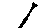
\includegraphics[scale=1.25]{figures/chapter3/elzehiry/insect-3.png}\quad\quad}
\end{tabular}
\caption{\textbf{Results for the grid graph model~\cite{zehiry10fast}.} The original image is displayed in the left; segmentation using only data in the middle; and the segmentation using squared curvature regularization in the right. Connectivity is encouraged, but to a very limited extension.}
\label{ch3:fig:elzehiry-results}
\end{figure}

In~\cite{nieuwenhuis14efficient} is presented an alternative formulation that is extendable to any desirable angle resolution. The idea is in fact quite similar to the one in~\cite{zehiry10fast} in the sense that curvature is measured by counting the number of configurations $(0,1,0)$ and $(1,0,1)$ of triplets of vertices. Intuitively, as illustrated in~\cref{ch3:fig:nieuweinhuis-triplets-1}, the curvature is higher at regions in which these configurations are more frequent. The authors prove the following theorem

\begin{figure}
\center
\subfloat[\label{ch3:fig:nieuweinhuis-triplets-1}]{
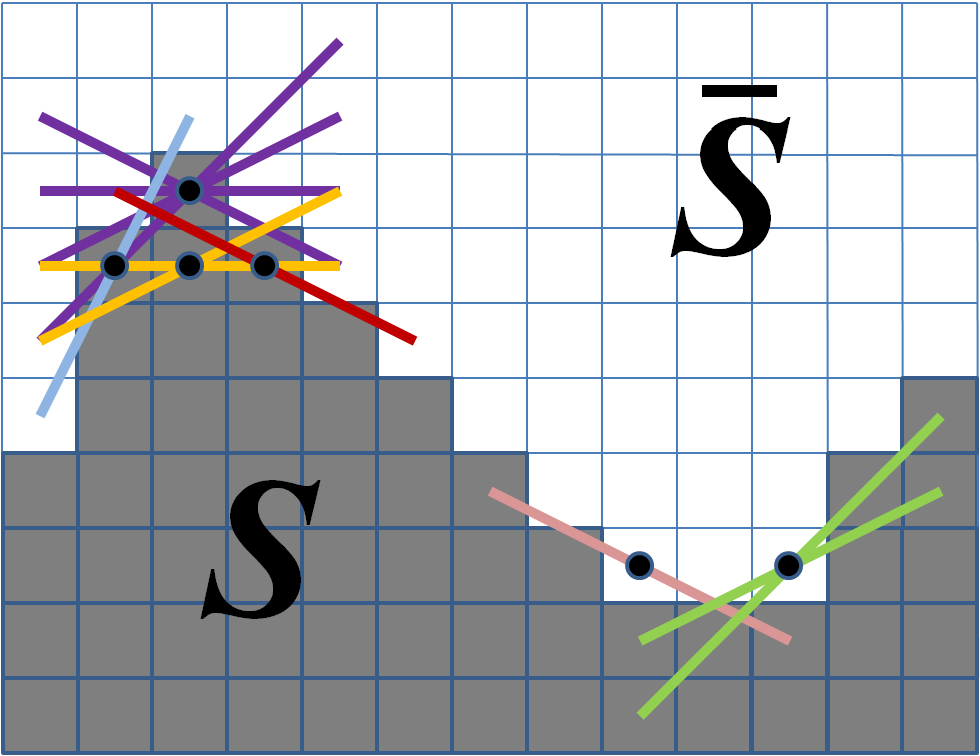
\includegraphics[scale=0.1]{figures/chapter3/nieuweinhuis/triplets.png}
}
\subfloat[\label{ch3:fig:nieuweinhuis-triplets-2}]{
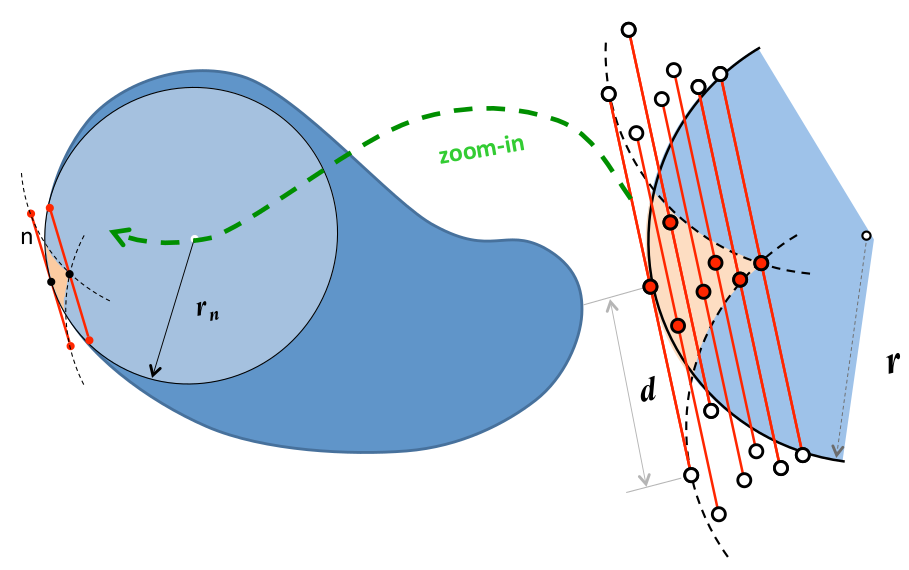
\includegraphics[scale=0.25]{figures/chapter3/nieuweinhuis/nieuwenhuis_brown_area.png}
}
\caption{\textbf{Triplets configurations and integral geometry~\cite{nieuwenhuis14efficient}.} In~\cref{ch3:fig:nieuweinhuis-triplets-1} we intuitively notice that curvature is higher where triplets configurations $(0,1,0)$ and $(1,0,1)$ are perceived. In~\cref{ch3:fig:nieuweinhuis-triplets-2}, an illustration of~\cref{ch3:thm:nieuweinhuis}. }
\label{ch3:fig:nieuweinhuis-triplets}
\end{figure}

\begin{theorem}{\cite{nieuwenhuis14efficient}}\label{ch3:thm:nieuweinhuis}
Let contour point $n$ have tangent orientation $t$ and osculating ball $B_r$ of radius $r=1/|k|$. Then, the set of all points $p \in B_r$ such that $\norm{p-n} \leq r$ and $(p \pm d \cdot t) \notin B_r$ for given distance $d < r$ has area 
\begin{align*}
	A(\kappa,d) &= \frac{|\kappa|d^3}{4} + O(d^4).
\end{align*}
%
\end{theorem}

Notice that the theorem is valid for cliques aligned with the tangent at the point of curvature computation. The set of available cliques orientations is defined according to the chosen neighborhood. The neighborhood system of size $(2d+1) \times (2d+1)$ for pixel $p$ is similar to a digital circle of radius $d$ centered at $p$ (although not the same), in the sense that the neighbors of $p$ are chosen in order to have approximately the same distance $d$ from $p$~(see~\cref{ch3:fig:nieuweinhuis-neighborhood}). The larger the value of $d$, the greater the chances to have a triplet orientation that matches the tangents along the object contour.

\begin{figure}
\center
\subfloat[$d=2$]{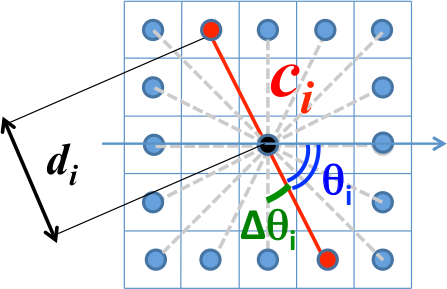
\includegraphics[scale=0.3]{figures/chapter3/nieuweinhuis/nieuwenhuis_neighborhood_1.png}
}\hspace{2em}
\subfloat[$d=3$]{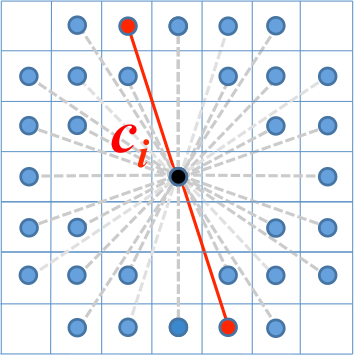
\includegraphics[scale=0.3]{figures/chapter3/nieuweinhuis/nieuwenhuis_neighborhood_2.png}
}
\caption{\textbf{Neighborhood system~\cite{nieuwenhuis14efficient}.} The higher the value of $d$, the higher is the angle resolution.}
\label{ch3:fig:nieuweinhuis-neighborhood}
\end{figure}

Let $d$ be the chosen neighborhood system and $c_i$ the corresponding triplets in this neighborhood. Moreover, assume that the triplets are ordered with respect the angle made with the horizontal axis. Let $\Delta \theta_i$ be the angle difference between two consecutive triplets and $i(p)$ the triplet index with the closest orientation to the tangent at $p$. The integral squared curvature is approximated by 
\begin{align*}
	\int_{C}{\kappa ^2 ds} &\approx \sum_{p}{ |\kappa_{p}|\Delta \theta_{i(p)}} \\
	&= \sum_{p} \frac{4\Delta \theta _{i(p)}}{d^3_{i(p)}} \cdot A(\kappa_p,d_{i(p)}) \\
	&\approx \sum_{i}\sum_{p} \frac{4\Delta \theta _i}{d^3_i} \cdot \delta(c_i(p)),
\end{align*}
%
where the function $\delta$ is one for triplets configurations $(0,1,0)$ or $(1,0,1)$ and zero otherwise. The function delta can be expressed as
\begin{align*}
	\delta(x_a,x_b,x_c) &= x_i(1-x_j)x_k + (1-x_i)x_j(1-x_k) \\
	&= x_j + x_ix_k - x_ix_j - x_jx_k.
\end{align*}
%
The resulting energy is non-submodular (the positive term in the $\delta$ function is non-submodular) and is solved using the LSA-TR method~\cite{gorelick14local}, reported to produce better results than QPBO for some non-submodular instances. Some results for inpainting and segmentation are shown in~\cref{ch3:fig:nieuweinhuis-results}. The model is unconstrained, extendable to arbitrary angle resolution and can be easily modified to include data and length terms. 
X
Although an argument is provided to justify the curvature approximation, it is difficult to do a multigrid analysis, i.e., to analyse its convergence over different resolutions. The experiments provided by the authors are limited to the computation of the elastica along a disk, and we are not sure about the behaviour of such estimator in shapes of more complex geometry. The fundamental goal of this thesis is to investigate imaging models using geometric penalization estimated by proven multigrid convergent estimators. In the next chapter we explore the multigrid convergence property and some other concepts of digital geometry.

\begin{figure}
\center
\begin{tabular}{ccc}
\subfloat[Original.]{
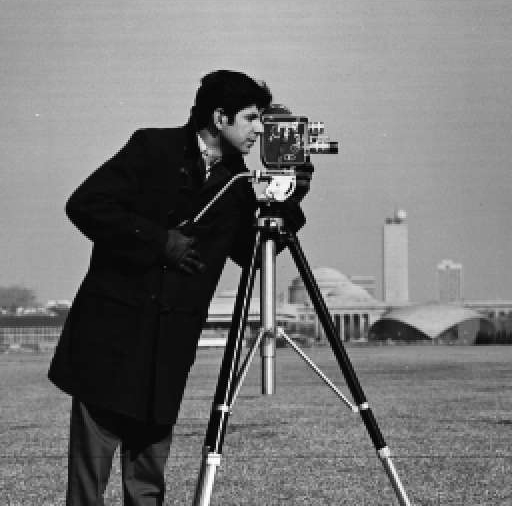
\includegraphics[scale=0.25]{figures/chapter3/nieuweinhuis/camera-man-1.png}} &
\subfloat[Binary segmentation.]{

\includegraphics[scale=0.25]{figures/chapter3/nieuweinhuis/camera-man-2.png}} &\\
\subfloat[Original and inpainting masks.]{
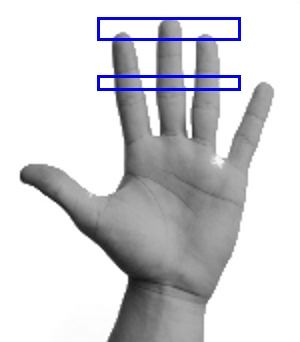
\includegraphics[scale=0.25]{figures/chapter3/nieuweinhuis/hand-1.png}} &
\subfloat[Inpainting with length regularization.]{\quad\quad
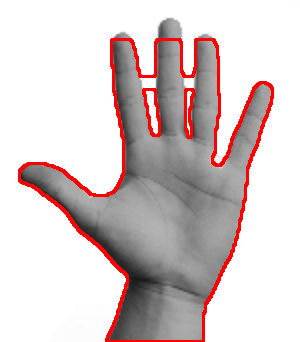
\includegraphics[scale=0.25]{figures/chapter3/nieuweinhuis/hand-2.png}\quad\quad} &
\subfloat[Inpainting with curvature regularization.]{
\includegraphics[scale=0.25]{figures/chapter3/nieuweinhuis/hand-3.png}}
\end{tabular}
\caption{\textbf{Segmentation and inpainting results~\cite{nieuwenhuis14efficient}.} The connectivity principle is perfectly illustrated in the inpainting problem but one would expect a completion of the rightmost bar of the camera tripod. }
\label{ch3:fig:nieuweinhuis-results}
\end{figure}



%
%\section{Chapter notes}
%
%the derived the following 
%
% to solve tasks as basic as edge detection. The curvature appeared in the context of diffusion methods, for example, consider the Perona-Malik edge detector. 
%
%Earlier appearances of curvature in image processing model dates back to the use
%
%The curvature appear in earlier models of image processing based on anisotropic diffusions. Take for example the edge detection task. The 
%
%The curvature is present in models of image processing even for the lowest-level tasks as edge detection. 
%
%Earlier models of image processing diffusion based 
%
%appears very often in models of image processing. 
%
%The curvature is presented in early models of image processing, some of them presented in~\cref{chapter:variational-methods-in-image-processing} as the Geometric Active Contour for image segmentation and Total Variation for image denoising.
%
%
%%\sketch{
%%\begin{enumerate}
%%	\item{Motivation}
%%	\item{Wave equation (Diprima)ter}
%%	\begin{itemize}
%%		\item{Curvature properties}
%%	\end{itemize}
%%	\begin{itemize}
%%		\item{Constraint optimization models}
%%		\item{Combinatorial optimization models}		
%%		\item{Continuous models}
%%	\end{itemize}
%%	
%%\end{enumerate}
%%}
%
%Por que nao usar diferencas finitas pra modelar curvatura ao quadrado?
%
%Por que nao usar elementos finitos para modelar curvatura ao quadrado?
%
%Qual o problema com a resolucao numerica de equacoes diferenciais de ordem alta?
%
%Inpainting de objetos com textura x objetos sem textura (PDE tende a suavizar em excesso e por isso nao seria apropriado para texturas. Mas o TV metodo eh capaz preservar em parte as discontinuidades. Bem, talvez em uma imagem super texturizada mesmo TV nao seja suficiente)
%
%Em PDEs de segunda ordem o passo do tempo artificial pode ser maior do que aquele de uma
%equacao de terceira ordem sem ter consequencias de divergencia.
%
%Mean curvature motion
%
%Derivacoes de curvatura. Curvatura de funcao implicita e a curvatura de level sets.
%
%Elastica. Derivacao do resultado da Free Elastica. Balloon and shrinking forces. Perimeter minimization is the energy being minimized by the mean curvature flow; the squared curvature term, on the other hand, contributes to grow the shape.
%
%
%Cubic splines and Elastica. Non linear splines study by Birkhof at General Motors.

	\chapter{Digital Geometry}
\label{chapter:digital-geometry}

\section{Ground concepts}

\section{Multigrid convergence}
\subsection{Multigrid convergence estimators}

\subsection{Tangent and perimeter estimators}	
\subsection{Curvature estimators}
	

\sketch{
\begin{enumerate}
	\item{Why a digital geometry?}
	\item{Digitization processes}
	\item{Geometric properties estimation}
	\item{Multigrid convergence}
	\item{Example of multigrid convergent estimators}
	\begin{itemize}
		\item{Tangent}
		\item{Perimeter}
		\item{Curvature}
	\end{itemize}	
\end{enumerate}
}
	\chapter{A combinatorial model for digital Elastica shape optimization}
\label{chapter:digital-elastica}

In this chapter we review the Elastica energy and some of its properties. Next, we introduce the digital version of the Elastica using multigrind convergent estimators of length and curvature. We present a combinatorial optimization model capable to evolve a shape to another of lower digital Elastica value. In several occasions, the final shape is indeed the optimal one, which confirms the pertinence of using multigrid convergent estimators to optimize geometric-related energies in digital sets. Finally, we present several attempts to derive a global model to minimize a simplification of the digital Elastica and we discuss why they fail.

\section{Continuous and digital Elastica}
\label{ch6:sec:continuous-digital-elastica}
	\sketch{To be further developed...}

	The Elastica energy of parameters $\Theta=(\alpha, \beta) \geq 0$ for some Euclidean shape $S \subset \mathbb{R}^2$ is defined as
	
	\begin{align*}
	E_{\Theta}(S) &= \int_{\partial S}{ \alpha + \beta \kappa(s)^2 ds}.
	\end{align*}
	
	
On the other hand, the digital Elastica $\hat{E}_{\Theta}$ of some digitization $D_h(S)$ of $S$ is defined as
	\begin{align}
	\hat{E}_{\Theta}( D_h(S) ) = \sum_{\dot{\vec{e}} \in \partial D_h(S)}{ \hat{s}( \dot{\vec{e}})\left(\; \alpha + \beta \hat{\kappa}_{r}^2(D_h(S),\dot{\vec{e}},h) \; \right)},
	\label{eq:digital-elastica}
	\end{align}
	
where $\dot{\vec{e}}$ denotes the center of the edge $\vec{e}$. In the
expression above, we will substitute an arbitrary subset $\Ds$ of
$\mathbb{Z}^2$ to $D_h(S)$ since the continuous shape $S$ is unknown.
In the following we omit the grid step $h$ to simplify expressions
(or, putting it differently, we assume that the shape of interest is
rescaled by $1/h$ and we set $h=1$). 

In the next section, we describe a combinatorial scheme that permit us to find the minimum digital shape with respect the digital Elastica energy for some neighborhood of shapes of $\Ds$. 

\section{Local combinatorial scheme}
\label{ch6:sec:local-combinatorial-scheme}

Given a digital shape $\Ds^{(0)}$ we describe a process that generates a
sequence $\Ds^{(i)}$ of shapes with non-increasing Elastica energy. The
idea is to define a neighborhood of shapes $\mathcal{N}^{(i)}$ to the
shape $\Ds^{(i)}$ and choose the element of $\mathcal{N}^{(i)}$ with
lowest energy.  The process is suited for the integral invariant
estimator but also for other curvature estimators, for example, MDCA
\cite{roussillon11mdca}. As a matter of fact, our experiments have
shown that either estimators induce similar results.

Let $\Ds$ be a $2$-dimensional digital shape embedded in a domain $\Omega \subset \mathbb{Z}^2$. We adopt the cellular-grid model to represent $\Ds$, i.e., pixels and its lower dimensional counterparts, linels and pointels, are part of $\Ds$ (see~\cref{fig:cellular-grid-model}). In particular, we denote by $\partial \Ds$ the topological boundary of $\Ds$, i.e., the connected sequence of linels such that for each linel we have one of its incident pixels in $\Ds$ and the other not in $\Ds$.

\begin{figure}[]
	\center
	\subfloat[\label{}]{%
	\includegraphics[scale=1.8]{figures/chapter5/cellular-grid/flower.png}
	}\hspace{40pt}%
	\subfloat[\label{}]{%	
	\includegraphics[scale=0.27]{figures/chapter5/cellular-grid/cellular-grid-illustration.pdf}
	}\hspace{40pt}%
	\subfloat[\label{}]{%
	\includegraphics[scale=0.035]{figures/chapter5/gcurves/distance-transform.pdf}
	}
	\caption{The flower shape in figure (a) and the cellular-grid model representation in (b) of the rectangle-bounded region. In figure (b), pixels are colored in gray, linels in green and pointels in blue. In figure (c), the blue pixels denotes a $3$-ring set.}
	\label{fig:cellular-grid-model}
\end{figure}

Let $d_{\Ds}:\Omega \rightarrow \mathbb{R}$ be the signed Euclidean distance transformation with respect to shape $\Ds$. The value $d_{\Ds}(p)$ gives the Euclidean distance between $p \notin \Ds$ and the closest pixel in $\Ds$. For points $p \in \Ds$, $d_{\Ds}(p)$ gives the distance between $p$ and the closest pixel not in $\Ds$.

\begin{definition}{m-Ring Set}
Given a digital shape $\Ds \in\Omega$, its signed distance transformation $d_{\Ds}$ and natural number $m \neq 0$, the {\em $m$-ring set of $\Ds$} is defined as
\begin{align*}
	R_m(\Ds) &:= L_m \cup L_{-m},
\end{align*}
where
\begin{align*}
	L_m(\Ds) &:= \left\{ \quad \begin{array}{cc}
		\left\{ p \in \Omega \; | \; m-1 < d_{\Ds}(p) \leq m \right\} & , \quad m>0\\
		\left\{ p \in \Omega \; | \; m+1 > d_{\Ds}(p) \geq m \right\} & , \quad m<0
		\end{array} \right.
\end{align*}
\end{definition}


Consider the following set of neighbor candidates to $\Ds$:
\begin{align*}
\mathcal{U}(\Ds) = \{ Q \; | \; Q \subset R_1(\Ds) \cup \Ds \; \text{and} \; \text{$Q$ is connected} \}.
\end{align*}


Such set can be extremely large and its complete exhaustion is prohibitively expensive.  Instead, we are going to use a subset of it.


\begin{definition}{$n$-neighborhood}

	Given a digital shape $\Ds \in \Omega$, its $n$-neigh\-bor\-hood $\mathcal{N}_n(\Ds)$ is defined as the set of digital shapes that can be built from $\Ds$ by adding or removing a sequence of $k \in [0,n]$ connected pixels in $R_1(\Ds)$.

\end{definition}



At first glance, we may be tempted to set the local-search neighborhood at the $k$-th iteration as the union of all $n$-neighborhood for $1<n<|\partial \Ds^{(k)}|$. However, that is often unecessary and timing consuming, as the greatest reduction in digital Elastica for a member of $\mathcal{N}_n$ is likely very close to the greatest reduction for a member of $\mathcal{N}_{n-1}$. Moreover, we can improve running time by implementing a multiscaling approach, i.e., we look for reductions in digital Elastica for larger values of $n$ first, and in case of a negative answer we refine our search by choosing a smaller $n$.

~\cref{alg:local-search} describes the local combinatorial process and is suitable for any type of digital estimator. To estimate length we use MDSS and to estimate curvature we execute~\cref{alg:local-search} with the MDCA and II-$r$ estimators ($r$ denoting the radius of the estimation ball) to solve the free and constrained Elastica problems. 
	

\begin{figure}[]
\center
\subfloat{
\includegraphics[scale=0.4]{figures/chapter5/gcurves/gc/main-inner.pdf}
}\hspace{1em}%
\subfloat{
\includegraphics[scale=0.4]{figures/chapter5/gcurves/gc/main-outer.pdf}
}\hspace{1em}\\[1em]
\subfloat{
\includegraphics[scale=0.4]{figures/chapter5/gcurves/gc/inner-main.pdf}
}\hspace{1em}%
\subfloat{
\includegraphics[scale=0.4]{figures/chapter5/gcurves/gc/outer-main.pdf}
}\hspace{1em}%
\caption{Members of $\mathcal{N}_{11}$ for the square shape.}
\end{figure}


\begin{algorithm}[H]
 \SetKwData{It}{k}
 \SetKwData{MIt}{maxIt}
 \SetKwData{Delta}{delta}
 \SetKwData{Best}{best} 
 \SetKwInOut{Input}{input}\SetKwInOut{Output}{output}
 \SetKwComment{comment}{//}{}
 
 \Input{A digital set $\Ds$; weight coefficients $\Theta=(\alpha , \beta)$; the number of curve segments $nc$; the maximum number of iterations \MIt}
 \BlankLine
 $t \longleftarrow 1$ \tcp*[l]{level of multiscaling}
 $k \longleftarrow 0$	\tcp*[l]{current iteration}
 $\Ds^{(0)} \longleftarrow \Ds$\;
 \While{ \It $<$ \MIt \bf{and} $t < \log_2{|\partial \Ds^{(k)}|}$ }
 { 	
	$M^{(k,t)}  \longleftarrow |\partial \Ds^{(k)}|/2^t$  	\tcp*[l]{Maximum $n$-neighborhood value.}
	
	$J \longleftarrow \{ j \cdot \frac{M^{(k,t)}}{nc} \; | \; 1 \leq j \leq nc \} $\;
	
	$\displaystyle \mathcal{N}^{(k,t)} \longleftarrow \displaystyle \Cup_{J}{\mathcal{N}_{j}(\Ds^{(k)})}$\;
	\BlankLine
	
	\comment{Find neighbor shape with lowest energy.} 
	$Q^{\star} \longleftarrow D^{(k-1)}$\;
  	\For{$ Q \in \mathcal{N}^{(k,t)} $}
	{
		\If{ $\hat{E}_{\Theta}(Q)$ $<$ $\hat{E}_{\Theta}(Q^\star)$ }
		{
			$Q^\star \longleftarrow Q$\; 
		}	
	}
	\BlankLine
	

	\Delta $\longleftarrow$ $\hat{E}_{\Theta}(\Ds^{(k-1)}) - \hat{E}_{\Theta}(\Ds^{(k)})$\;	
	
	\If{ \Delta $\leq 0$ } 
	{
		\comment{Better solution not found. Refine the scale.}
		$t \longleftarrow t+1$ 
	}		
	\Else 
	{ 
		\comment{Better solution found. Set $D^{(k)}$ and reset multiscaling.}
		$t \longleftarrow 1$\;	
		$\Ds^{(k)} \longleftarrow Q^\star$\;
		\It $\longleftarrow$ \It $+1$\;		
	}
	
 }
 \caption{LocalSearch algorithm for Elastica minimization.}
  \label{alg:local-search} 
\end{algorithm}

\subsection{Free digital Elastica}
\label{ch6:subsec:free-digital-elastica}
In the free digital Elastica energy we optimize~\cref{eq:digital-elastica} without any constraint. We observe that for $\alpha=0, \beta >0$ the Elastica becomes the integration of the squared curvature  along the shape contour which has the ball of infinite radius as its minimizer. For $\alpha > 0, \beta=0$, minimize Elastica becomes minimize perimeter (curvature flow). It is easy to see that for $\alpha, \beta > 0$, the optimal shape for the Elastica is a disk of radius $r$. We can easily find the value of $r$.

\begin{align*}
	\frac{d}{dr}\big( \int_{\partial B(r)}{ (\alpha + \beta \kappa ^2) ds} \big ) &= 0\\
	\frac{d}{dr}\big( \alpha 2\pi r + \beta \pi/r \big) &= 0\\
	r &= \alpha^{-1/2}.
\end{align*}  

Therefore, the optimal shape for the free digital Elastica is a digital disk of finite radius $\alpha^{-1/2}$.


In~\cref{fig:local-comb-estimators-plots-lp001} we present the digital Elastica evolution for parameters $\alpha=0.01, \beta=1$ and three different curvature estimators in three different scales. The shapes evolution using the II-$5$ estimator are shown in~\cref{fig:local-comb-ii5-results}. We observe that both II-$5$ and II-$10$ evolve the shapes to disks of radius close to the optimum value of $10$. The II-$3$ estimator stops prematurely at a local optimum due its limited sensibility compared to II-$5$ or II-$10$, while MDCA encounters some difficults to evolve in a high resolution setting and it also stops at some local optimum. In fact, the MDCA estimator, although with higher convergence speed, is more sensitive to noise than II, as illustrated in~\cref{fig:mdca-sensitivity}. Nonetheless, the results can be improved by using a larger neighborhood, as illustrates~\cref{fig:mdca-larger-neighborhood}.



We have executed the same experiments for different parameters $\alpha$ to confirm the effectiveness of our approach. We observe that the plots for $\alpha=0.001$ in~\cref{fig:local-comb-estimators-plots-lp0001} follows a pattern similar to those in~\cref{fig:local-comb-estimators-plots-lp001} for $\alpha=0.01$. In particular, the remarks for the II-$3$ and MDCA estimator are the same. Further, we point out that II-$5$ values are slightly farther from the optimum for $\alpha=0.001$. The reason being that the shapes evolve to a ball of higher radius compared to the case $\alpha=0.01$. At some point of the evolution for $\alpha=0.001$, the sensibility of II-$5$ is not sufficient to escape from local optimum. We remark that the adoption of an automatic selection of the estimation ball radius may attenuate this problem.



\begin{figure}[]
\center
\subfloat{
\includegraphics[scale=0.4]{figures/chapter5/flow/plots/bars/length_pen_0.01000/triangle.pdf}
}\hspace{1em}%
\subfloat{
\includegraphics[scale=0.4]{figures/chapter5/flow/plots/bars/length_pen_0.01000/square.pdf}
}\hspace{1em}%
\subfloat{
\includegraphics[scale=0.4]{figures/chapter5/flow/plots/bars/length_pen_0.01000/flower.pdf}
}\hspace{1em}%
\subfloat{
\includegraphics[scale=0.4]{figures/chapter5/flow/plots/bars/length_pen_0.01000/bean.pdf}
}\hspace{1em}%
\subfloat{
\includegraphics[scale=0.4]{figures/chapter5/flow/plots/bars/length_pen_0.01000/ellipse.pdf}
}\hspace{1em}%
\subfloat{
\includegraphics[scale=0.4]{figures/chapter5/flow/plots/summary/lp_0.01/summary-ii5.pdf}
}%
\caption{Minimum value attained for the digial Elastica ($\alpha=0.01, \beta=1$) in comparisson with the global optimium (dashed line) for different curvature estimators and in different scales. The last figure summarizes the digital Elastica evolution value for all shapes using grid step $h=0.25$.}
\label{fig:local-comb-estimators-plots-lp001}
\end{figure}

\begin{figure}[]
\center
\subfloat{
\includegraphics[scale=0.4]{figures/chapter5/flow/plots/bars/length_pen_0.00100/triangle.pdf}
}\hspace{1em}%
\subfloat{
\includegraphics[scale=0.4]{figures/chapter5/flow/plots/bars/length_pen_0.00100/square.pdf}
}\hspace{1em}%
\subfloat{
\includegraphics[scale=0.4]{figures/chapter5/flow/plots/bars/length_pen_0.00100/flower.pdf}
}\hspace{1em}%
\subfloat{
\includegraphics[scale=0.4]{figures/chapter5/flow/plots/bars/length_pen_0.00100/bean.pdf}
}\hspace{1em}%
\subfloat{
\includegraphics[scale=0.4]{figures/chapter5/flow/plots/bars/length_pen_0.00100/ellipse.pdf}
}\hspace{1em}%
\subfloat{
\includegraphics[scale=0.4]{figures/chapter5/flow/plots/summary/lp_0.001/summary-ii5.pdf}
}%
\caption{Minimum value attained for the digial Elastica ($\alpha=0.001, \beta=1$) in comparisson with the global optimium (dashed line) for different curvature estimators and in different scales. The last figure summarizes the digital Elastica evolution value for all shapes using grid step $h=0.25$.}
\label{fig:local-comb-estimators-plots-lp0001}
\end{figure}


\begin{figure}[hp!]
	\center
	\begin{tabular}{ccc}
		$h=1.0$ & $h=0.5$ & $h=0.25$ \\[2em]
	\includegraphics[scale=0.185]{figures/chapter5/flow/triangle/radius_5/ii/elastica/len_pen_0.01000/jonctions_1/curve_segs_4/best/gs_1.00000/summary.pdf} &
	\includegraphics[scale=0.185]{figures/chapter5/flow/triangle/radius_5/ii/elastica/len_pen_0.01000/jonctions_1/curve_segs_4/best/gs_0.50000/summary.pdf} &
	\includegraphics[scale=0.185]{figures/chapter5/flow/triangle/radius_5/ii/elastica/len_pen_0.01000/jonctions_1/curve_segs_4/best/gs_0.25000/summary.pdf}\\[2em]
		
	\includegraphics[scale=0.17]{figures/chapter5/flow/square/radius_5/ii/elastica/len_pen_0.01000/jonctions_1/curve_segs_4/best/gs_1.00000/summary.pdf} &
	
	\includegraphics[scale=0.17]{figures/chapter5/flow/square/radius_5/ii/elastica/len_pen_0.01000/jonctions_1/curve_segs_4/best/gs_0.50000/summary.pdf} &	
	
	\includegraphics[scale=0.17]{figures/chapter5/flow/square/radius_5/ii/elastica/len_pen_0.01000/jonctions_1/curve_segs_4/best/gs_0.25000/summary.pdf}\\[2em]
	
	
	\includegraphics[scale=0.25]{figures/chapter5/flow/flower/radius_5/ii/elastica/len_pen_0.01000/jonctions_1/curve_segs_4/best/gs_1.00000/summary.pdf} &		
	
	\includegraphics[scale=0.25]{figures/chapter5/flow/flower/radius_5/ii/elastica/len_pen_0.01000/jonctions_1/curve_segs_4/best/gs_0.50000/summary.pdf} &

	\includegraphics[scale=0.25]{figures/chapter5/flow/flower/radius_5/ii/elastica/len_pen_0.01000/jonctions_1/curve_segs_4/best/gs_0.25000/summary.pdf}\\[2em]	
	
	\includegraphics[scale=0.25]{figures/chapter5/flow/bean/radius_5/ii/elastica/len_pen_0.01000/jonctions_1/curve_segs_4/best/gs_1.00000/summary.pdf} &	 
	
	\includegraphics[scale=0.25]{figures/chapter5/flow/bean/radius_5/ii/elastica/len_pen_0.01000/jonctions_1/curve_segs_4/best/gs_0.50000/summary.pdf} &	
	
	\includegraphics[scale=0.25]{figures/chapter5/flow/bean/radius_5/ii/elastica/len_pen_0.01000/jonctions_1/curve_segs_4/best/gs_0.25000/summary.pdf}\\[2em]			

	
	\includegraphics[scale=0.25]{figures/chapter5/flow/ellipse/radius_5/ii/elastica/len_pen_0.01000/jonctions_1/curve_segs_4/best/gs_1.00000/summary.pdf} &

	\includegraphics[scale=0.25]{figures/chapter5/flow/ellipse/radius_5/ii/elastica/len_pen_0.01000/jonctions_1/curve_segs_4/best/gs_0.25000/summary.pdf} &

	\includegraphics[scale=0.25]{figures/chapter5/flow/ellipse/radius_5/ii/elastica/len_pen_0.01000/jonctions_1/curve_segs_4/best/gs_0.25000/summary.pdf}				
\end{tabular}
		\caption{LocalSearch algorithm evolutions for several shapes with $\alpha=0.01,\beta=1$. The initial contour is colored in red; the final contour is colored in blue; and the optimal contour is colored in green.}	
		\label{fig:local-comb-ii5-results}
\end{figure}

\begin{figure}
\center
\begin{tabular}{cccc}
& $h=1.0$ & $h=0.5$ & $h=0.25$\\[2em]
\multirow{2}{*}{\rotatebox{90}{$n$-neighborhood}} & 
\figTable{0.25}{figures/chapter5/flow/triangle/radius_3/mdca/elastica/len_pen_0.01000/jonctions_1/curve_segs_4/best/gs_1.00000/summary.pdf} &
\figTable{0.25}{figures/chapter5/flow/triangle/radius_3/mdca/elastica/len_pen_0.01000/jonctions_1/curve_segs_4/best/gs_0.50000/summary.pdf} &
\figTable{0.25}{figures/chapter5/flow/triangle/radius_3/mdca/elastica/len_pen_0.01000/jonctions_1/curve_segs_4/best/gs_0.25000/summary.pdf}\\
& \figTable{0.25}{figures/chapter5/flow/flower/radius_3/mdca/elastica/len_pen_0.01000/jonctions_1/curve_segs_4/best/gs_1.00000/summary.pdf} &
\figTable{0.25}{figures/chapter5/flow/flower/radius_3/mdca/elastica/len_pen_0.01000/jonctions_1/curve_segs_4/best/gs_0.50000/summary.pdf} &
\figTable{0.25}{figures/chapter5/flow/flower/radius_3/mdca/elastica/len_pen_0.01000/jonctions_1/curve_segs_4/best/gs_0.25000/summary.pdf}\\[8em]

\hline\\[2em]

\multirow{2}{*}{\rotatebox{90}{Extended $n$-neighborhood}} & 
\figTable{0.25}{figures/chapter5/mdca-larger-neighborhood/triangle/0.01/1.0/summary.pdf} &
\figTable{0.25}{figures/chapter5/mdca-larger-neighborhood/triangle/0.01/0.5/summary.pdf} &
\figTable{0.25}{figures/chapter5/mdca-larger-neighborhood/triangle/0.01/0.25/summary.pdf}\\

& \figTable{0.25}{figures/chapter5/mdca-larger-neighborhood/flower/0.01/1.0/summary.pdf} &
\figTable{0.25}{figures/chapter5/mdca-larger-neighborhood/flower/0.01/0.5/summary.pdf} &
\figTable{0.25}{figures/chapter5/mdca-larger-neighborhood/flower/0.01/0.25/summary.pdf}


\end{tabular}
\caption{In the top row, the MDCA evolution for the neighborhood as presented in~\cref{alg:local-search}. In the bottom row, the flow using the extended neighborhood. The extended neighborhood additionaly includes the $n$-neighborhood of the dilation and the erosion of the initial shape by a square of side $1$.}
\label{fig:mdca-larger-neighborhood}
\end{figure}



\begin{figure}[]
\begin{minipage}[b]{0.6\textwidth}
\center
\includegraphics[scale=0.15]{figures/chapter5/mdca-sensitivity/closer-picture.pdf}
\end{minipage}%
\begin{minipage}[b]{0.4\textwidth}
\center
\includegraphics[scale=0.025]{figures/chapter5/mdca-sensitivity/big-picture.pdf}\\\vspace{2em}
\captionsetup{type=table}
\begin{tabular}{r|c|c}
& II-$5$ & MDCA \\
\hline
Red  & 5.54 & 3.93\\
Blue & 5.55 & 3.84\\
\hline
$| \Delta E / \Delta \Ds |$ & 70 & 1400
\end{tabular}
\end{minipage}
\caption{A slight variation in the shape boundary (in this example, a $0.07\%$ change or $4$ pixels over $5310$) inflicts a considerably higher change in the energy value when using MDCA than when using II. }
\label{fig:mdca-sensitivity}
\end{figure}

\subsection{Constrained digital Elastica}
\label{ch6:subsec:constrained-digital-elastica}

An important advantage of~\cref{alg:local-search} is that constraints can be imposed with minimum effort. We present results for two types of constraints. In the first type, we force some pixels to be part of the final solution and in the second we impose orientations at the endpoints of a curve. In~\cref{fig:constrained-elastica} we compare the flows for different values of $\alpha$.

We remark that~\cref{alg:local-search} is sensitive to the parameter $\alpha$. For higher values of $\alpha$, the shapes tends to shrink and the curves are closer to a straight line. For lower values of $\alpha$, the shapes tends to grow and the curves make more turns. 

\begin{figure}
\center
\begin{tabular}{ccc}
$\alpha=0.1$ & $\alpha=0.01$ & $\alpha=0.001$\\[2em]
\includegraphics[scale=0.25]{figures/chapter5/fixed-pixels/elastica/len_pen_0.1/flower-1/summary.pdf} &
\includegraphics[scale=0.25]{figures/chapter5/fixed-pixels/elastica/len_pen_0.01/flower-1/summary.pdf} &
\includegraphics[scale=0.25]{figures/chapter5/fixed-pixels/elastica/len_pen_0.001/flower-1/summary.pdf}\\[2em]
\includegraphics[scale=0.25]{figures/chapter5/fixed-pixels/elastica/len_pen_0.1/flower-2/summary.pdf} &
\includegraphics[scale=0.25]{figures/chapter5/fixed-pixels/elastica/len_pen_0.01/flower-2/summary.pdf} &
\includegraphics[scale=0.25]{figures/chapter5/fixed-pixels/elastica/len_pen_0.001/flower-2/summary.pdf}\\[2em]
\includegraphics[scale=0.25]{figures/chapter5/fixed-orientations/elastica/len_pen_0.1/curve-2/summary.pdf} &
\includegraphics[scale=0.25]{figures/chapter5/fixed-orientations/elastica/len_pen_0.01/curve-2/summary.pdf} &
\includegraphics[scale=0.25]{figures/chapter5/fixed-orientations/elastica/len_pen_0.001/curve-2/summary.pdf}\\[2em]
\includegraphics[scale=0.25]{figures/chapter5/fixed-orientations/elastica/len_pen_0.1/curve-3/summary.pdf} &
\includegraphics[scale=0.25]{figures/chapter5/fixed-orientations/elastica/len_pen_0.01/curve-3/summary.pdf} &
\includegraphics[scale=0.25]{figures/chapter5/fixed-orientations/elastica/len_pen_0.001/curve-3/summary.pdf}
\end{tabular}
\caption{In the first and second rows, the flow obtained by forcing the green pixels to be part of the final solution; In the last two rows, the flow obtained by forcing the orientation at the endpoints of the curves.}
\label{fig:constrained-elastica}

\end{figure}

\subsection{Running time}
\label{ch6:subsec:running-time}

The running time of~\cref{alg:local-search} is summarized in table~\cref{tab:summary-local-comb-rtime}. All the experiments in this thesis were executed on a $32$-core $2.4Ghz$ CPU. Although its use in practical applications is
limited, we demonstrated that digital estimators are effective in their measurements and the flows evolve as expected, reaching the global optimum for some shapes. We
observe that it is a complete digital approach, and we do not suffer from discretization and rounding problems, a common
issue in continuous models.  Furthermore we have checked that this approach works indifferently with Integral Invariant
curvature estimator and Maximal Digital Circular Arc curvature estimator, given an appropriate neighborhood. So the convergence of the digital curvature
estimator seems to be the cornerstone to get a digital curve behaving like a continuous Elastica. 

\begin{figure}[h!]
\center
\captionsetup{type=table}
\begin{tabular}{|l|c|c|c|c|c|c|}
\hline
& \multicolumn{2}{c|}{$h=1.0$} & \multicolumn{2}{c|}{$h=0.5$} & \multicolumn{2}{c|}{$h=0.25$}\\
\hline
& Pixels & Time & Pixels & Time & Pixels & Time\\
\hline
Triangle & 521 & 2s (0.07s/it)  & 2080 & 43s (0.81s/it) & 8315 & 532s(4.8s/it)\\
Square & 841 & 0.9s (0.09s/it) & 3249 & 8s (0.3s/it) & 12769 & 102s (2s/it)\\
Flower & 1641 & 13s (0.24s/it) & 6577 & 209s (1.68s/it) & 26321 & 3534s (12.3s/it)\\
Bean  & 1574 & 7s (0.16s/it) & 6278 & 88s (1.08s/it) & 25130 & 1131s (6.4s/it)\\
Ellipse  & 626 & 1s (0.14s/it) & 2506 & 16s (0.44s/it) & 10038 & 286s (3.1s/it)\\
\hline
\end{tabular}
\caption{Running time of LocalSearch for the free Elastica problem.}
\label{tab:summary-local-comb-rtime} 
\end{figure}





\section{Global optimization}
\label{ch6:sec:global-optimization}

In this section we turn to a global optimization approach. However, instead of minimizing~\cref{eq:digital-elastica} we are going to optimize a simplified version of it in which we don't need to compute the local length estimator.

\subsection{Simplified digital Elastica}
\label{ch6:subsec:simplified-digital-elastica}

The simplified digital Elastica is defined as

	\begin{align}
	\hat{E}_{\Theta}^{simp}( D_h(S) ) = \sum_{\dot{\vec{e}} \in \partial D_h(S)}{ \alpha + \beta \hat{\kappa}_{r}^2(D_h(S),\dot{\vec{e}},h) }.
	\label{eq:simplified-digital-elastica}
	\end{align}
	

We argue that~\cref{eq:simplified-digital-elastica} is a reasonable approximation of~\cref{eq:digital-elastica}. Indeed, executing~\cref{alg:local-search} for minimize the simplified digital Elastica obtains very similar results to those for the digital Elastica (see~\cref{fig:simplified-elastica}).


\begin{figure}[]
\center
\begin{tabular}{ccc}
\includegraphics[scale=0.25]{figures/chapter5/flow/triangle/radius_5/ii/selastica/len_pen_0.01000/jonctions_1/curve_segs_4/best/gs_0.25000/summary.pdf} &
\includegraphics[scale=0.25]{figures/chapter5/flow/square/radius_5/ii/selastica/len_pen_0.01000/jonctions_1/curve_segs_4/best/gs_0.25000/summary.pdf} &
\includegraphics[scale=0.25]{figures/chapter5/flow/ellipse/radius_5/ii/selastica/len_pen_0.01000/jonctions_1/curve_segs_4/best/gs_0.25000/summary.pdf}\\[2em]
\includegraphics[scale=0.25]{figures/chapter5/flow/flower/radius_5/ii/selastica/len_pen_0.01000/jonctions_1/curve_segs_4/best/gs_0.25000/summary.pdf} &
\includegraphics[scale=0.25]{figures/chapter5/flow/bean/radius_5/ii/selastica/len_pen_0.01000/jonctions_1/curve_segs_4/best/gs_0.25000/summary.pdf} &
\includegraphics[scale=0.25]{figures/chapter5/fixed-pixels/selastica/len_pen_0.01/flower-1/summary.pdf}\\[2em]
\includegraphics[scale=0.25]{figures/chapter5/fixed-pixels/selastica/len_pen_0.01/flower-2/summary.pdf} &
\includegraphics[scale=0.25]{figures/chapter5/fixed-orientations/selastica/len_pen_0.01/curve-2/summary.pdf} &
\includegraphics[scale=0.25]{figures/chapter5/fixed-orientations/selastica/len_pen_0.01/curve-3/summary.pdf}
\end{tabular}
\caption{Experiments of~\cref{ch6:sec:local-combinatorial-scheme} for the simplified digital Elastica.}
\label{fig:simplified-elastica}
\end{figure}


\subsection{Optimization model for simplified digital Elastica}
\label{ch6:subsec:optimization-model-simplified-digital-elastica}

Differently from the previous section, the model described here is designed for the integral invariant estimator only. Let $\Ds \in \frac{1}{2}\mathbb{Z}^2$ be the digitization of some shape $S \in \mathbb{R}^2$ using grid step $h$ in half-integer coordinates space. We assume that $\Ds$ has $m$ pixels (located at integer coordinates) and $n$ linels (one and only one of its coordinates is $\frac{1}{2}$). Optimization variables are represented as column vectors $\vec{x} \in \mathbb{B}^{m},\, \vec{y} \in \mathbb{B}^{n}$ and its $i$-th coefficients are denoted  $\vec{x}_i,\vec{y}_i$.  Further, let $\vec{A} \in \mathbb{B}^{m\times n}$ the matrix defined as

\[
	\vec{A}_{i,j} = \left\{ \begin{array}{ll}
		1,\; x_j \in B_{r}(y_i)\\
		0,\; \text{otherwise}.
	\end{array}\right.
\]

In other words, the column vector $\vec{A}_i$ of $\vec{A}$ represents the pixels that are in the interior of the disk $B_{r}(y_i)$ of radius $r$ centered at $\vec{y}_i$. 


\begin{align}
	E_{\Theta}^{simp}(\vec{x},\vec{y}) =& \sum_{\vec{y}_i \in \vec{y}}{ \vec{y}_i \left(\; \alpha + \beta \hat{\kappa}_{r}^2(D,\vec{y}_i) \; \right)}\\\nonumber
			   =& \sum_{\vec{y}_i \in \vec{y}}{ \vec{y}_i \left(\; \alpha  + \beta \big( \frac{3}{r^3}(\frac{\pi}{r^2} - |B_r(\vec{y}_i)|)\big)^2\right)}\\\nonumber
			   =& \sum_{\vec{y}_i \in \vec{y}}{ \vec{y}_i \left(\; \alpha + \frac{9}{r^6}\beta \big(c^2 - 2c\vec{A}_i^T\vec{x} + \vec{x}^T\vec{A}_i\vec{A}_i^T\vec{x}\big)\right)},			   
	\end{align}
	
where $c =  \pi r^2/2$. We remark that linels and pixels in the solution must be topologicaly consistent, .i.e., linels must form connected closed curves and the pixels must lie in the interior of those curves. This restriction is encoded in a set of topological constraints $T(x,y)$ detailed later. So far we have

\begin{align*}
	\min_{\vec{x} \in \mathbb{B}^{|X|}, \vec{y} \in \mathbb{B}^{|Y|}}{E_{\Theta}^{simp}(\vec{x},\vec{y})}, \quad \text{subject to } T(\vec{x},\vec{y}). \quad (P0)
\end{align*}

Additionaly, in real applications involving the minimization of Elastica, we have a set of constraints $R$ that plays the role of regularization. For example, we may force some of the pixels in the original shape to be part of the solution; for imaging problems, we may add a data attachment term, and so on. Finally, we can write the general optimization problem as

\begin{align*}
	\min_{\vec{x} \in \mathbb{B}^{|X|}, \vec{y} \in \mathbb{B}^{|Y|}}{E_{\Theta}^{simp}(\vec{x},\vec{y})}, \quad \text{subject to } T(\vec{x},\vec{y}), R(x) \quad (P1)
\end{align*}

	Formulation $P1$ is a constrained binary non-convex third order problem and likely difficult to be solved optimally. Nonetheless, we can use standard optimization techniques to acquire some intuition on the model. 	
	
\subsection{Topological constraints}
\label{ch6:subsec:topological-constraints}

The estimation ball should be applied in the digital boundary of the shape, which oblige us to impose topological constraints in the model to avoid inconsistent solutions. In order to accomplish that, we set an arbitrary orientation for the faces and another for the edges. We choose counter-clockwise for faces; left-to-right for horizontal edges; and bottom-to-up for vertical edges.


We create the vector $\vec{z} \in \mathbb{B}^{2n}$. We map each linel identified by variable $\vec{y}_i$ to components $\vec{z}_{2i},\vec{z}_{2i+1}$, one for each possible orientation the linel may assume. Next, we extend the linel incidence matrix defined in~\cref{app:pixel-incidence-matrix} to hold incidence with respect to oriented edges. The new matrix $\vec{T} \in \mathbb{B}^{n \times m + 2n}$ is defined as

\[
	0 \leq j < m, \quad \vec{T}_{i,j} = \left\{ \begin{array}{ll}
	
	1,& \text{Pixel $j$ is positively incident to linel $i$}\\
	-1,& \text{Pixel $j$ is negatively incident to linel $i$}\\	
	0,& \text{otherwise},
	\end{array}\right.
\]

\[
	m \leq j < m + 2n, \quad \vec{T}_{i,j} = \left\{ \begin{array}{ll}
	
	1,& \text{Edge $j$ is positively incident to linel $i$}\\
	-1,& \text{Edge $j$ is negatively incident to linel $i$}\\	
	0,& \text{otherwise}.
	\end{array}\right.
\]

Rewriting formulation (P1)

\[
\begin{array}{ll}
& \displaystyle	\min \sum_{z_i \in \vec{z}}{ \vec{z}_i \left(\; \alpha + \frac{9}{r^6}\beta \big(c^2 - 2c\vec{A}_i^T\vec{x} + \vec{x}^T\vec{A}_i\vec{A}_i^T\vec{x}\big)\right)} \\
\text{subject to}\\
&	\vec{T} \times  \left[ \begin{array}{c}
							\vec{x} \\ 
							\vec{z} 
						   \end{array} \right] = 0 \\
&   R(\vec{x}),\\
&   \vec{x} \in \mathbb{B}^{m}, \vec{z} \in \mathbb{B}^{2n}.
\end{array}
\]


We observe that for a linel identified by variable $\vec{y}_i$, constraints $\vec{T}$ forces at most one of the variables $\vec{z}_{2i},\vec{z}_{2i+1}$ to be evaluated to one. 


\subsection{Linear relaxation of $P1$}
\label{ch6:subsec:linear-relaxation}

	The simplest model we can derive from (P1) consists in to relax the optimization variables, i.e., we impose $\vec{x} \in \mathbb{U}^m$ and $\vec{z} \in \mathbb{U}^{2n}$, and we linearize all second and third order terms. 
	
	Consider the summation in (P1). An opt-term is an ordered sequence of optimization variables, e.g., the opt-term $\vec{x}_2^2\vec{x}_4$ is encoded as the sequence $(\vec{x}_2,\vec{x}_2,\vec{x}_4)$. Let $\mathcal{T}$ the collection of opt-terms of order two or higher in (P1) and $\mathcal{T}_i \in \mathcal{T}$ a member of this collection. To linearize (P1), we associate a variable $\vec{u_i}$ for each term of $\mathcal{T}$, i.e., $\vec{u} \in \mathbb{U}^{|\mathcal{T}|}$ and we enforce $|\mathcal{T}_i|+1$ new constraints. In other words, we add the following set of linearization constraints.
	
\[
	L(\vec{u}) = \left\{ \Big\{ \vec{u}_i \leq t, \quad \forall t \in \mathcal{T}_i \Big\} \cup \Big\{ \vec{u}_i \geq \displaystyle \sum_{t \in \mathcal{T}_i}{t} - |\mathcal{T}_i| + 1 \Big\} \; \Big| \; \forall \mathcal{T}_i \in \mathcal{T} \right\}
\]

The linearization of (P1) is written as

\[
\begin{array}{ll}
& \displaystyle	\min \sum_{z_i \in \vec{z}}{ \vec{z}_i \left(\; \alpha + \frac{9}{r^6}\beta \big(c^2 - 2c\vec{A}_i^T\vec{x} + \vec{x}^T\vec{A}_i\vec{A}_i^T\vec{x}\big)\right)} \\
\text{subject to}\\
&	\vec{T} \times  \left[ \begin{array}{c}
							\vec{x} \\ 
							\vec{z} 
						   \end{array} \right] = 0 \\
&   R(\vec{x}),\\
&   L(\vec{u}),\\
&   \vec{x} \in \mathbb{U}^{m}, \vec{z} \in \mathbb{U}^{2n}, \vec{u} \in \mathbb{U}^{|\mathcal{T}|} 
\end{array}
\]

	Finally, to obtain a binary vector we round the partial solution vector $\vec{x^{\star}} \in \mathbb{U}^m$. For an instance with $m$ pixels we have about $2m$ linels. After linearization, we can expect to have up to $O(m^3)$ variables, dampening our attempts to solve it globally even for low resolution images. One can also try quadratic formulations by linearizing only the third order terms. Unfortunately, the matrix of quadratic terms is not semi-definite positive, fundamental condition for efficient optimization of the model.
	


\subsection{Unconstrained version of P1}
\label{ch6:subsec:unconstrained-version}

We can use the pixel incidence matrix defined in~\cref{app:pixel-incidence-matrix} to define an unconstrained version of P1. The pixel incidence vector $\vec{q} \in \mathbb{Z}^m$ for pixels $\vec{x} \in \mathbb{B}^{m}$ is 
	
	\begin{align*}
		\vec{q} &= \vec{P}^T\vec{P} \vec{x}
	\end{align*}

In order to supress the sign, we define diagonal matrix $\vec{Q} \in \mathbb{R}^{m \times m }$ as

\begin{align*}
	\vec{Q} = diag(\vec{q})diag(\vec{q})
\end{align*}

Let $\vec{B} \in \mathbb{B}^{m\times m}$ such that column vector $\vec{B}_j$ represents the pixels in the interior of a disk of radius $R$ centered at pixel $i$. Finally, we search for solutions of

\begin{align}
	\min_{\vec{x}} \frac{9}{R^6}\sum_{j}^{m}{\left( \frac{\pi R^2}{2} - \frac{1}{2}\boldsymbol{\mathbf{1}}^T{\vec{Q}}\vec{B}_j \right)^2},
	\label{eq:unconstrained-digital-elastica}
\end{align}


where $\mathbf{1} = (1,1, \cdots , 1)^T \in \mathbb{R}^m$. ~\cref{eq:unconstrained-digital-elastica} involves the minimization of a fourth order equation and therefore hard to be optimized.

\section{Conclusion}
\label{ch6:sec:conclusion}
We gave a historical review of the Elastica and we defined the digital Elastica energy in~\cref{ch6:sec:continuous-digital-elastica}. The local combinatorial scheme defined in~\cref{ch6:sec:local-combinatorial-scheme} can evolve different shapes guided by the minimization of digital Elastica energy and it eventually reaches global optimum in the free Elastica problem, justifying the interest for multigrid convergent estimators. The model can also be used to solve the constrained Elastica problem, but its more likely to stop in a local optimum. Finnaly, we sketch some global optimization models in~\cref{ch6:sec:global-optimization} for minimizing the simplified Elastica using standard techniques of optimization. The difficulties we pointed out suggest that a practical global optimization model is unlikely to exist. In the next chapter we explore a model that decreases the Elastica energy and that can be used in practice.


	\chapter{A 2-step evolution model driven by digital elastica minimization}
\chaptermark{A 2-step evolution model}
\label{chapter:flip-flow}

In the previous chapter we have presented a local combinatorial model using multigrid convergent estimator that proved to be very successful in optimizing the digital elastica but too slow to be used in practice. We have also attempted to derive a global optimization model, but unfortunately such model is unlikely to be solved in the current state of art of binary optimization techniques. In this chapter we present a second local optimization model that is much faster than~\cref{ch5:alg:local-search} but with fewer guarantees of optimality.

\daniel{
We describe the binary non-submodular FlipFlow energy and discuss some curious aspects of it in~\cref{ch6:sec:flipflow-model}. Optimization strategies are presented in~\cref{ch6:sec:optimization-method,ch6:sec:evaluation-across-rings}. Finally, we describe an application of the FlipFlow model to image segmentation in~\cref{ch6:sec:data-term-image-segmentation}.
}


\section{FlipFlow model}
\label{ch6:sec:flipflow-model}

In this section we describe the FlipFlow model that aims to evolve an initial digital shape $\Ds$ into another of lower digital elastica value. The FlipFlow algorithm consists into deciding, at each iteration $k$, which pixels in the \emph{inner boundary} of $\Ds^{(k)}$ are to be removed  and which are to be kept. 

\subsection{Definitions}
\label{ch6:subsec:definitions}

Let $\Ds$ be a digital shape with domain $\Omega \subset \mathbb{Z}^2$. We describe a flow $\left \{ \Ds^{(k)} \; | \; k \geq 0, \Ds^{0} = \Ds \right\}$ intended to decrease the digital elastica energy of $\Ds$.

We assume an ordering in $\Omega$, i.e., there exists a bijective function $\omega : \Omega \rightarrow \{1 \cdots |\Omega| \}$. Moreover, let $X_{\omega}:\Omega \rightarrow 2^{\{0,1\}}$ be an operator that transforms digital sets in its corresponding set of binary variables, i.e.,
\begin{align*}
	X_{\omega}(\Omega) := \left\{ x_{\omega(p)} \in \{0,1\} \; | \; p \in \Omega \right\}.
\end{align*}
%
We will simply write $X(\Omega)$, assuming that exists an underlying ordering function $\omega$.

A $\{0,1\}$ assignment of the variables in $X(\Omega)$ is denoted $x(\Omega)$. We define the sum of a digital set $\Ds$ and an assignment $x(\Omega)$ as
\begin{align*}
	\Ds + x(\Omega) = \Ds \cup \left\{ p \; | \; p \in P, x_{\omega(p)}=1 \right\}.
\end{align*}
%
Next, we define the set of optimization variables. In order to guarantee connectivity and thus avoid the enforcement of the topological constraints discussed in~\cref{ch5:subsec:topological-constraints}, we limit the optimization region to a subset of $\Omega$, namely the inner pixel boundary of  $\Ds^{(k)}$. \daniel{We recall the definition given in~\cref{chapter:digital-elastica}}.
\begin{align*}
	I(\Ds) := \left\{ \: p \; | \; p \in \Ds, |\mathcal{N}_4(x) \cap \Ds|<4 \: \right\},
\end{align*}
%
%Further, we write $\overline{I}(\Ds)$ to denote the inner pixel boundary of the complement of $\Ds$, i.e., $\overline{I}(\Ds) := I(\overline{\Ds})$.
%
To simplify notation, the inner pixel boundary of $\Ds^{(k)}$ is simply denoted $I^{(k)}$. At each iteration, the set $X^{(k)}$ of optimization variables is defined as
\begin{align*}
	X^{(k)} := X(I^{(k)}).
\end{align*}
%
In the case we optimize the complement of $\Ds$, we write $\overline{X}^{(k)}$, i.e., $\overline{X}^{(k)} = X(I(\overline{\Ds}^ {(k)}))$.

An assignment of $X^{(k)}$ is simply denoted $x^{(k)}$. 


\subsection{\daniel{Model and algorithm}}
\label{ch6:subsec:algorithm}

We recall the definition of the II digital curvature estimator \daniel{(see~\cref{ch4:sec:geometric-measurements} for details):}
\begin{align}
	\hat{\kappa}^2(p) &= c_1\Big( c_2 - | B_r(p) \cap \Ds^{(k)} | \Big)^2, 
	\label{eq:curvature-estimator-pixels}
\end{align}
where $c_1=3/r^6$ and $c_2=\pi r^2/2$. 
%
The following sets are important in the expansion of $~\cref{eq:curvature-estimator-pixels}$.
\begin{align*}
	\begin{array}{rll}
	F^{(k)} &:= \Ds^{(k)} \setminus I^{(k)} & \text{ \daniel{(Sure foreground) }} \\
	F_r^{(k)}(p) &:= F^{(k)} \cap B_r(p) &\\
	I_r^{(k)}(p) &:= I^{(k)} \cap B_r(p) & \\
	X_r^{(k)}(p) &:= X\big( I_r^{(k)}(p) \big). & \\	
	\end{array}
\end{align*}
%
%
Expanding~\cref{eq:curvature-estimator-pixels}, we get 
\begin{align}
  \hat{\kappa}^2(p) &= c_1\Big( c_2 - |F_{r}^{(k)}(p)| - \sum_{x_j \in X_r^{(k)}(p)} {x_j} \Big)^2 \nonumber \\
   &= c_1 \Big( C + 2\left( |F_{r}^{(k)}(p)| - c_2 \right) \hspace{-2mm}\sum_{x_j \in X_{r}^{(k)}(p)}\hspace{-2mm}{x_j} + \hspace{-2mm}\sum_{x_j \in X_{r}^{(k)}(p)}\hspace{-2mm}{x_j^2} + \hspace{-2mm}\sum_{ \substack{x_j,x_l \in X_{r}^{(k)}(p) \\ j<l} }\hspace{-2mm}{2x_jx_l}  \Big),
   \label{eq:digital-squared-curvature-term}
\end{align}
where $C=c_2^2 - 2c_2 \cdot |F_{r}^{(k)}(p)| + |F_{r}^{(k)}(p)|^2$ is a constant. As~\cref{eq:digital-squared-curvature-term} is a term to be optimized, we can ignore constants and multiplication factors. Moreover, as we are in a binary optimization setting, we can  further simplify~\cref{eq:digital-squared-curvature-term} by exploiting the binary character of variables and eliminating monomials of second order. We define the following family
of energies for given parameters $\vec{\theta}=(\alpha,\beta ) \geq 0$ \daniel{and $m \geq 0$}
\begin{align}
  E_{(\vec{\theta},m)}^{flip}(\Ds^{(k)},X^{(k)}) =& \sum_{x_j \in X^{(k)}}{\alpha s(x_j)} + \nonumber \\ 
  & \sum_{ \substack{p \in \\ \daniel{R_m(\Ds^{(k)})}}}{ 2c_1 \beta  \Big( { (1/2+ |F_{r}^{(k)}(p)|-c_2) \cdot \sum_{ \substack{ x_j \in \\ X_{r}^{(k)}(p)}}{x_j} } + \sum_{ \substack{j<l, \\ x_j,x_l \in \\ X_{r}^{(k)}(p) } }{x_jx_l} \Big) },
  \label{eq:energy-family}
\end{align}
where $s(\cdot)$ denotes the length penalization term, written as
\begin{align}
  s(x_{w(p)})=\sum_{q \in \mathcal{N}_4(p)}{ t(q) }, \quad \text{where } t(q) = \left\{\begin{array}{ll}
  (x_{w(p)}-x_{w(q)})^2, & \text{if } q \in I^{(k)}\\
  (x_{w(p)}-1)^2, & \text{if } q \in F^{(k)}\\
  (x_{w(p)}-0)^2, & \text{otherwise. }
  \end{array}\right.
  \label{eq:length-penalization}
\end{align}
%
%
We recall that $R_m$ refers to the $m$-ring defined in~\cref{ch5:sec:local-combinatorial-scheme}. Each choice of $m$ generates a different flow, which is generally described in the \emph{FlipFlow}~\cref{ch6:alg:evolution-model}. To optimize~\cref{eq:energy-family} we use the QPBOI algorithm \cite{rother07qpbo}.


\begin{algorithm}
 \SetKwData{It}{k}
 \SetKwData{MIt}{maxIt}
 \SetKwData{Delta}{delta}
 \SetKwInOut{Input}{input}\SetKwInOut{Output}{output}
 \SetKwComment{comment}{//}{}
 
 \Input{A digital set $\Ds$; The ring number $m$; Length($\alpha$), curvature($\beta$) grouped in parameter vector $\vec{\theta}$; the maximum number of iterations \MIt;}
 \BlankLine
 $\Ds^{(0)} \longleftarrow \Ds$\;
 $k \longleftarrow 1$\;
 \While{ \It $<$ \MIt  }{ 	
	\comment{Shrink mode}
	\If{ \It is even }{	 
	 	$x^{(k-1)} \longleftarrow \displaystyle \argmin_{X^{(k-1)}} E_{(\vec{\theta},m)}^{flip}(\Ds^{(k-1)},1-X^{(k-1)})$\; 	
 		$\Ds^{(k)} \longleftarrow F^{(k-1)} + x^{(k-1)}$\;
 	}
	\comment{Expansion mode} 	
 	\Else{	
	 	$\overline{x}^{(k-1)} \longleftarrow \displaystyle \argmin_{\overline{X}^{(k-1)}} E_{(\vec{\theta},m)}^{flip}(\Ds^{(k-1)},1-\overline{X}^{(k-1)})$\;
 		$\Ds^{(k)} \longleftarrow \overline{ \overline{F}^{(k-1)} + \overline{x}^{(k-1)}}$\; 	
 	}
 	
	\It $\longleftarrow$ \It $+1$\;
	
 }
 \caption{FlipFlow algorithm.}
 \label{ch6:alg:evolution-model}  
\end{algorithm}

\subsection{Algorithm discussion}
\label{ch6:subsec:flipflow-algorithm-discussion}

\begin{figure}
\begin{minipage}{0.49\textwidth}
\center
\includegraphics[scale=0.15]{figures/chapter6/contour-information/before-opt.pdf}
\label{ch6:fig:contour-info-1}
\end{minipage}%
\begin{minipage}{0.49\textwidth}
\center
\includegraphics[scale=0.15]{figures/chapter6/contour-information/after-opt.pdf}
\label{ch6:fig:contour-info-2}
\end{minipage}%
\caption{ \daniel{\textbf{Fixed boundary evaluation.}} The proposed model does not take contour information into account, thus the II curvature estimator is evaluated and optimized with respect the initial boundary. In the left, the initial shape and the optimization variables colored in yellow. In the right, the final shape without taking the complementary solution.}
\label{ch6:fig:contour-info}
\end{figure}
\daniel{We are going to justify~\cref{ch6:alg:evolution-model} considering the case in which $m=0$, i.e., for energy $E_{\theta,0}^{flip}$. } As discussed in~\cref{ch5:sec:global-optimization}, the topological constraints are a fundamental part in a global optimization model for the digital elastica but the complexity added to it dampens any hope of optimizing it efficiently. In the proposed FlipFlow model, we exclude topological constraints and we end up with the tractable binary second order~\cref{eq:energy-family}. However, due the lack of contour information, the minimization of~\cref{eq:energy-family} for $\Ds^{(k)}$ results in undesirable shapes of even higher digital elastica energy values  (see~\cref{ch6:fig:contour-info}). Interestingly, by using the inverse of the optimal assignement, we can derive a shape of lower digital elastica energy. Therefore, the next shape is given by
\begin{align*}
	\Ds^{(k+1)} = \daniel{F^{(k)} + } \argmin _{}{E_{(\vec{\theta},m)}^{flip}\big(\Ds^{(k)},1-X^{(k)}} \big).
\end{align*}
%
Recall that the integral invariant estimator approaches curvature by computing the difference between half of the area
of a chosen ball and the area of the intersection of this ball with the shape.  In particular, regions of positive
curvature have fewer pixels in their intersection set than on its complement w.r.t the estimation ball. This implies
that variables in such regions are labeled with 1, as the unbalance grows otherwise. We attenuate curvature if we shift
the center of the estimation ball towards the interior of the shape, which means to remove the 1-labeled pixels. That is
why we take the complement of the optimization solution.


The explanation above covers the treatment of convex parts, but the way to treat concavities is not much different. Indeed, concave regions are convex in the shape complement. The FlipFlow~\cref{ch6:alg:evolution-model} is made of two modes: shrink and expansion. The shrink mode handles convexities and its reasoning is explained in the last paragraph. The expansion mode operates exactly in the same way, but at the image complement, and by doing this we are able to handle
concavities. It is called expansion mode because the optimization region, in this case, is the outer pixel boundary of
the original shape. Table~\cref{tab:flow-summary} sums up these arguments.

%Length and data terms should be properly defined in order to comply with the complement step of the FlipFlow
%algorithm. The length penalization is defined as
%
%\begin{align}
%  s(x_{w(p)})=\sum_{q \in \mathcal{N}_4(p)}{ t(q) }, \quad \text{where } t(q) = \left\{\begin{array}{ll}
%  (x_{w(p)}-x_{w(q)})^2, & \text{if } q \in I^{(k)}\\
%  (x_{w(p)}-0), & \text{if } q \in F^{(k)}\\
%  (x_{w(p)}-1), & \text{otherwise }
%  \end{array}\right.
%  \label{eq:length-penalization}
%\end{align}
%
\begin{table}
  \center
  \setlength{\extrarowheight}{0.75em}
  \begin{tabular}{|c|c|c|c|} \hline
    shrink mode &    $\kappa \gg 0$ & $\kappa \geq 0$ &  $\kappa < 0$ \\ \hline
    $x^{(k)}$ & $x_j=1$ & $x_j \in \{0,1\}$ & $x_j=0$ \\ \hline
    $\Ds^{(k+1)} \leftarrow F^{(k)} + x^{(k)}$ & eroded & prob. eroded & unchanged  \\ \hline \hline
    expansion mode &    $\overline{\kappa} \gg 0$ & $\overline{\kappa} \geq 0$ & $\overline{\kappa} < 0$ \\ \hline
    $\overline{x}^{(k)}$ & $\overline{x}_j=1$ & $\overline{x}_j \in \{0,1\}$ & $\overline{x}_j=0$ \\ \hline
    $\Ds^{(k+1)} \leftarrow \overline{\overline{F}^{(k)} + \overline{x}^{(k)}}$ & dilated & prob. dilated & unchanged \\ \hline 
  \end{tabular}
  
  \caption{ \daniel{\textbf{Shrink and expansion modes.}} Since the curvature is negated when reversing the curve (i.e. $\overline{\kappa}=-\kappa$), this process can only shrink  convex parts in shrink mode and expand concave parts in expansion mode.}
   \label{tab:flow-summary}	  

\end{table}


In~\cref{ch6:fig:m1-square-flow} we show the results of the FlipFlow algorithm for $( \daniel{m=0}, \alpha=\{0, 0.5\}, \beta=1 )$. We observe a global evolution towards rounder shapes, but several artifacts are formed along the boundary. An estimation ball of higher radius evolves the shapes faster, but the contours become noisier. Setting $\alpha >0$ attenuates the problem for lower radius but the produced shapes does not match with our intuition of what a flow driven by the squared curvature must be like. In the next section we investigate how the energy properties and optimization method used can explain this behavior.

\begin{figure}
\center
\begin{tabular}{p{2.5em}ccc}
& $r=3$ & $r=5$ & $r=9$ \\[2em]
\multirow{2}{*}{$\alpha=0$}& \includegraphics[scale=0.25]{figures/chapter6/radius-effect/triangle/improve/len_pen0/radius-3/summary.pdf} &
\includegraphics[scale=0.23]{figures/chapter6/radius-effect/triangle/improve/len_pen0/radius-5/summary.pdf} &
\includegraphics[scale=0.23]{figures/chapter6/radius-effect/triangle/improve/len_pen0/radius-9/summary.pdf} \\[2em]
& \includegraphics[scale=0.23]{figures/chapter6/radius-effect/flower/improve/len_pen0/radius-3/summary.pdf} &
\includegraphics[scale=0.23]{figures/chapter6/radius-effect/flower/improve/len_pen0/radius-5/summary.pdf} &
\includegraphics[scale=0.23]{figures/chapter6/radius-effect/flower/improve/len_pen0/radius-9/summary.pdf} \\
\hline \\
\multirow{2}{*}{$\alpha=0.5$}& \includegraphics[scale=0.25]{figures/chapter6/radius-effect/triangle/improve/len_pen0.5/radius-3/summary.pdf} &
\includegraphics[scale=0.23]{figures/chapter6/radius-effect/triangle/improve/len_pen0.5/radius-5/summary.pdf} &
\includegraphics[scale=0.23]{figures/chapter6/radius-effect/triangle/improve/len_pen0.5/radius-9/summary.pdf} \\[2em]
& \includegraphics[scale=0.23]{figures/chapter6/radius-effect/flower/improve/len_pen0.5/radius-3/summary.pdf} &
\includegraphics[scale=0.23]{figures/chapter6/radius-effect/flower/improve/len_pen0.5/radius-5/summary.pdf} &
\includegraphics[scale=0.23]{figures/chapter6/radius-effect/flower/improve/len_pen0.5/radius-9/summary.pdf}
\end{tabular}

\caption{\daniel{\textbf{FlipFlow results for $m=0,\beta=1$.}} The algorithm is very sensitive to the little variations of the estimator, which are particularly important in regions of low squared curvature. Artifacts are somewhat reduced with a length penalization but increases if we use a higher ball radius. For better visualization, curves are displayed every $1/10$ of the number of iterations. }
\label{ch6:fig:m1-square-flow}
\end{figure}


%\begin{figure}
%\center
%\subfloat[]{
%\includegraphics[scale=0.45]{figures/chapter6/radius-effect/triangle/improve/len_pen0/radius-3/radius-effect.pdf}}%
%\subfloat[]{
%\includegraphics[scale=0.45]{figures/chapter6/radius-effect/flower/improve/len_pen0/radius-3/radius-effect.pdf}}%
%\caption{The digital elastica decreases in a turbulent way.}
%\end{figure}


\section{Optimization method}
\label{ch6:sec:optimization-method}

Let $f$ be a function of $n$ binary variables with unary and pairwise terms, i.e.
\begin{align*}
f(y_1,\cdots, y_n) = \sum_{j}{f_j(y_j)} + \sum_{j < k}{f_{j,k}(y_j,y_k)}.
\end{align*}
%
\daniel{As described in~\cref{ch2:sec:submodular-functions},} function $f$ is submodular if and only if the following inequality holds for each pairwise term $f_{j,k}$: %\cite{kolmogorov04whatenergies}
\begin{align*}
  \quad f_{j,k}(0,0) + f_{j,k}(1,1) \leq f_{j,k}(0,1) + f_{j,k}(1,0).
\end{align*}
%
The energy $E_{(\vec{\theta},m)}^{flip}$ is non-submodular and optimizing it is a difficult problem, which constrains us to use heuristics and
approximation algorithms. The QPBO method \cite{hammer84} transforms the original problem in a max-flow/min-cut
formulation and yields a full optimal labeling for submodular energies. For non-submodular energies the method is
guaranteed to return a partial labeling with the property that the set of labeled variables is part of an optimal
solution. That property is called partial optimality.

In practice, QPBO can leave many pixels unlabeled. There exist two extensions to QPBO that alleviate this limitation:
QPBOI (improve) and QPBOP (probe) \cite{rother07qpbo}. The first is an approximation method that is guaranteed to not increase the energy,
but loses the property of partial optimality. The second is an exact method which is reported to label more variables
than QPBO.

The percentage of unlabeled pixels by QPBOP for $E_{(\vec{\theta},m)}^{flip}$ is quite high, but the percentage decreases to zero as we set $m$
to a value closer to $r$, the estimation ball radius. Therefore, we are more confident in taking the solution for values of $m$ close to $r$. However, the way it
varies across values of $m$ differs from shape to shape, as is illustrated in~\cref{ch6:fig:unlabeled-versus-iterations}. We also noticed that, for $m=r$, all the pixels were labeled, which
  indicates that $E_{(\vec{\theta},r)}^{flip}$ is an easy instance of the general non-submodular energy $E_{(\vec{\theta},m)}^{flip}$, but this remains to be
  proved. The number of pairwise terms in $E_{(\vec{\theta},r)}^{flip}$ is roughly half of those in $E_{(\vec{\theta},1)}^{flip}$ (see~\cref{ch6:fig:ratio-pairwise-terms}), which also explains the higher number of labeled variables.

  We have used QPBOI to solve $E_{(\vec{\theta},m)}^{flip}$. Naturally, in the case where all pixels are labeled by QPBOP, QPBOI returns the same labeling as QPBOP. In the next section we show that by evaluating the estimation ball at outer rings, we eliminate the artifacts and we produce smoother flows while preserving a qualitative measure of curvature.
  
  \daniel{We postpone the comparison of the proposed methods in this thesis to~\cref{chapter:results-analysis}. At this point, we retain us to say that the FlipFlow performs up to 10x faster than the LocalSearch algorithm.} 


\begin{figure}
\center
\includegraphics[scale=0.5]{figures/chapter6/unlabeled-ratio/plots/pairwise-ratio/h0.25/radius-5/plot-pairwiseratio-lowerHigher-concavities-probe.pdf}
\caption{\daniel{\textbf{Pairwise terms ratio}.}We plot the ratio of pairwise terms among all $\binom{|X^{(k)}|}{2}$ combinations. The highest ring has roughly half the number of pairwise terms as the lowest ring.}
\label{ch6:fig:ratio-pairwise-terms}
\end{figure}


\begin{figure}
\center
\begin{minipage}[b]{0.5\textwidth}
%\subfloat[]{ \includegraphics[scale=0.38]{figures/chapter6/unlabeled-ratio/plots/unlabeled-per-iterations/h0.25/radius-3/plot-model-triangle-concavities-probe.pdf}}\\%
\subfloat[]{ \includegraphics[scale=0.38]{figures/chapter6/unlabeled-ratio/plots/unlabeled-per-iterations/h0.25/radius-5/plot-model-triangle-concavities-probe.pdf}}\\%
\subfloat[]{ \includegraphics[scale=0.38]{figures/chapter6/unlabeled-ratio/plots/unlabeled-per-iterations/h0.25/radius-9/plot-model-triangle-concavities-probe.pdf}}%
\end{minipage}%
\begin{minipage}[b]{0.5\textwidth}
%\subfloat[]{ \includegraphics[scale=0.38]{figures/chapter6/unlabeled-ratio/plots/unlabeled-per-iterations/h0.25/radius-3/plot-model-flower-concavities-probe.pdf}}\\%
\subfloat[]{ \includegraphics[scale=0.38]{figures/chapter6/unlabeled-ratio/plots/unlabeled-per-iterations/h0.25/radius-5/plot-model-flower-concavities-probe.pdf}}\\%
\subfloat[]{ \includegraphics[scale=0.38]{figures/chapter6/unlabeled-ratio/plots/unlabeled-per-iterations/h0.25/radius-9/plot-model-flower-concavities-probe.pdf}}%
\end{minipage}
\caption{\daniel{\textbf{Unlabeled variables ratio across $m$-rings.}}For each plot, we first produce the sequence of shapes $\left\{ \Ds^{(k)} \right\}$ executing FlipFlow with $m=r$. Then, for each shape in $\left\{ \Ds^{(k)} \right\}$, we execute one iteration of FlipFlow for different values of $m$ and we count the unlabeled pixels. The number of unlabeled pixels by QPBOP remains high for lower values of $m$, and goes to zero when $m=r$. %We observe the same behavior for varying radius values.
}
\label{ch6:fig:unlabeled-versus-iterations}
\end{figure}



\section{Evaluation across $m$-rings}
\label{ch6:sec:evaluation-across-rings}

%\begin{figure}
%\center
%\begin{tabular}{p{3em}ccc}
%$m=1$ & \includegraphics[scale=0.22]{figures/chapter6/level-effect/triangle/improve/len_pen0/radius-5/level1/summary.pdf} &
%\includegraphics[scale=0.22]{figures/chapter6/level-effect/flower/improve/len_pen0/radius-5/level1/summary.pdf} &
%\includegraphics[scale=0.22]{figures/chapter6/level-effect/bean/improve/len_pen0/radius-5/level1/summary.pdf} \\[2em]
%$m=3$ & \includegraphics[scale=0.22]{figures/chapter6/level-effect/triangle/improve/len_pen0/radius-5/level3/summary.pdf} &
%\includegraphics[scale=0.22]{figures/chapter6/level-effect/flower/improve/len_pen0/radius-5/level3/summary.pdf} &
%\includegraphics[scale=0.22]{figures/chapter6/level-effect/bean/improve/len_pen0/radius-5/level3/summary.pdf} \\[2em]
%$m=4$ & \includegraphics[scale=0.22]{figures/chapter6/level-effect/triangle/improve/len_pen0/radius-5/level4/summary.pdf} &
%\includegraphics[scale=0.22]{figures/chapter6/level-effect/flower/improve/len_pen0/radius-5/level4/summary.pdf} &
%\includegraphics[scale=0.22]{figures/chapter6/level-effect/bean/improve/len_pen0/radius-5/level4/summary.pdf} \\[2em]
%$m=5$ & \includegraphics[scale=0.22]{figures/chapter6/level-effect/triangle/improve/len_pen0/radius-5/level5/summary.pdf} &
%\includegraphics[scale=0.22]{figures/chapter6/level-effect/flower/improve/len_pen0/radius-5/level5/summary.pdf} &
%\includegraphics[scale=0.22]{figures/chapter6/level-effect/bean/improve/len_pen0/radius-5/level5/summary.pdf} \\[2em]
%\end{tabular}
%\caption{\daniel{\textbf{FlipFlow results for $\mathbf{r=5}$.}} By positioning the estimation ball on outer rings, we minimize artifacts creation. %The radius of the estimation ball used here equals to $5$ and the curves are displayed every $10$ iterations.
%}
%\label{ch6:fig:mrings-r5-evolution}
%\end{figure}
%
%
%\begin{figure}
%\center
%\begin{tabular}{p{3em}ccc}
%$m=1$ & \includegraphics[scale=0.22]{figures/chapter6/level-effect/triangle/improve/len_pen0/radius-9/level1/summary.pdf} &
%\includegraphics[scale=0.22]{figures/chapter6/level-effect/flower/improve/len_pen0/radius-9/level1/summary.pdf} &
%\includegraphics[scale=0.22]{figures/chapter6/level-effect/bean/improve/len_pen0/radius-9/level1/summary.pdf} \\[2em]
%$m=5$ & \includegraphics[scale=0.22]{figures/chapter6/level-effect/triangle/improve/len_pen0/radius-9/level5/summary.pdf} &
%\includegraphics[scale=0.22]{figures/chapter6/level-effect/flower/improve/len_pen0/radius-9/level5/summary.pdf} &
%\includegraphics[scale=0.22]{figures/chapter6/level-effect/bean/improve/len_pen0/radius-9/level5/summary.pdf} \\[2em]
%$m=8$ & \includegraphics[scale=0.22]{figures/chapter6/level-effect/triangle/improve/len_pen0/radius-9/level8/summary.pdf} &
%\includegraphics[scale=0.22]{figures/chapter6/level-effect/flower/improve/len_pen0/radius-9/level8/summary.pdf} &
%\includegraphics[scale=0.22]{figures/chapter6/level-effect/bean/improve/len_pen0/radius-9/level8/summary.pdf} \\[2em]
%$m=9$ & \includegraphics[scale=0.22]{figures/chapter6/level-effect/triangle/improve/len_pen0/radius-9/level9/summary.pdf} &
%\includegraphics[scale=0.22]{figures/chapter6/level-effect/flower/improve/len_pen0/radius-9/level9/summary.pdf} &
%\includegraphics[scale=0.22]{figures/chapter6/level-effect/bean/improve/len_pen0/radius-9/level9/summary.pdf} \\[2em]
%\end{tabular}
%\caption{\daniel{\textbf{FlipFlow results for $\mathbf{r=9}$.}} By positioning the estimation ball on outer rings, we minimize artifacts creation. %The radius of the estimation ball used here equals to $9$ and the curves are displayed every $10$ iterations.
%}
%\label{ch6:fig:mrings-r9-evolution}
%\end{figure}



\begin{figure}
\center
\begin{tabular}{ccc}
$m=1$ & $m=4$ & $m=5$\\
\includegraphics[scale=0.22]{figures/chapter6/level-effect/triangle/improve/len_pen0/radius-5/level1/summary.pdf} &
\includegraphics[scale=0.22]{figures/chapter6/level-effect/triangle/improve/len_pen0/radius-5/level4/summary.pdf} &
\includegraphics[scale=0.22]{figures/chapter6/level-effect/triangle/improve/len_pen0/radius-5/level5/summary.pdf}\\[2em]
\includegraphics[scale=0.22]{figures/chapter6/level-effect/flower/improve/len_pen0/radius-5/level1/summary.pdf} &
\includegraphics[scale=0.22]{figures/chapter6/level-effect/flower/improve/len_pen0/radius-5/level4/summary.pdf} &
\includegraphics[scale=0.22]{figures/chapter6/level-effect/flower/improve/len_pen0/radius-5/level5/summary.pdf} 
\end{tabular}
\caption{\daniel{\textbf{FlipFlow results for $\mathbf{r=5}$.}} By positioning the estimation ball on outer rings, we minimize artifacts creation. %The radius of the estimation ball used here equals to $5$ and the curves are displayed every $10$ iterations.
}
\label{ch6:fig:mrings-r5-evolution}
\end{figure}


\begin{figure}
\center
\begin{tabular}{ccc}
$m=1$ & $m=6$ & $m=9$\\
\includegraphics[scale=0.22]{figures/chapter6/level-effect/triangle/improve/len_pen0/radius-9/level1/summary.pdf} &
\includegraphics[scale=0.22]{figures/chapter6/level-effect/triangle/improve/len_pen0/radius-9/level6/summary.pdf} &
\includegraphics[scale=0.22]{figures/chapter6/level-effect/triangle/improve/len_pen0/radius-9/level9/summary.pdf}\\[2em]
\includegraphics[scale=0.22]{figures/chapter6/level-effect/flower/improve/len_pen0/radius-9/level1/summary.pdf} &
\includegraphics[scale=0.22]{figures/chapter6/level-effect/flower/improve/len_pen0/radius-9/level6/summary.pdf} &
\includegraphics[scale=0.22]{figures/chapter6/level-effect/flower/improve/len_pen0/radius-9/level9/summary.pdf}
\end{tabular}
\caption{\daniel{\textbf{FlipFlow results for $\mathbf{r=9}$.}} By positioning the estimation ball on outer rings, we minimize artifacts creation. %The radius of the estimation ball used here equals to $9$ and the curves are displayed every $10$ iterations.
}
\label{ch6:fig:mrings-r9-evolution}
\end{figure}




\begin{figure}
\center
\subfloat[]{
\includegraphics[scale=0.4]{figures/chapter6/level-effect/triangle/improve/len_pen0/radius-5/level1/level-effect.pdf}}%
\subfloat[]{
\includegraphics[scale=0.4]{figures/chapter6/level-effect/triangle/improve/len_pen0/radius-9/level1/level-effect.pdf}}%


\subfloat[]{
\includegraphics[scale=0.4]{figures/chapter6/level-effect/flower/improve/len_pen0/radius-5/level1/level-effect.pdf}}%
\subfloat[]{
\includegraphics[scale=0.4]{figures/chapter6/level-effect/flower/improve/len_pen0/radius-9/level1/level-effect.pdf}}%
\caption{\daniel{\textbf{Digital elastica evaluation.} We present the results of the FlipFlow model for different values of $m$. %h=0.25
In the left column, we use FlipFlow radius $5$ and in the right column we use FlipFlow radius $9$. }}
\label{ch6:fig:mrings-plots-r5-r9}
\end{figure}

\begin{figure}
\center
\subfloat[]{\includegraphics[scale=0.7]{figures/chapter6/topology-change/summary-wave.pdf}}

\subfloat[]{\includegraphics[scale=0.2]{figures/chapter6/topology-change/summary-square-holes.pdf}}
\caption{\daniel{\textbf{Evolution speed and topology changes.}} The flow evolves regions of high curvature faster, as illustrated in figure (a). Figure (b) illustrates the property of the FlipFlow algorithm to handle changes in topology.}
\label{ch6:fig:handle-topology-different-speed}
\end{figure}

\begin{figure}
\center
\begin{tabular}{cccc}
\multirow{2}{*}{Seeds} & \multirow{2}{*}{Graph cut} & $\alpha=0.5, \beta=0.0,$ & $\alpha=0.5, \beta=1.0,$ \\
& & $\gamma=0.5$ & $\gamma=0.5$\\
 	\includegraphics[scale=0.25]{figures/chapter6/segmentation/coala/mt_improve/radius_5/data_0.50/sq_0.00/length_0.50/it_50/seeds.png} & 
 	\includegraphics[scale=0.25]{figures/chapter6/segmentation/coala/mt_improve/radius_5/data_0.50/sq_0.00/length_0.50/it_50/gc-seg.png} & 
 	\includegraphics[scale=0.25]{figures/chapter6/segmentation/coala/mt_improve/radius_5/data_0.50/sq_0.00/length_0.50/it_50/corrected-seg.png} & 
 	\includegraphics[scale=0.25]{figures/chapter6/segmentation/coala/mt_improve/radius_5/data_0.50/sq_1.00/length_0.50/it_50/corrected-seg.png}
\end{tabular}	
\caption{Given foreground (green) and background (blue) seeds at picture (a); Graph cut produces picture (b) which is used as input of the Contour Correction algorithm; in pictures (c) and (d) we display the output of Contour Correction algorithm with and without squared curvature regularization. }
\label{ch6:fig:segmentation}
\end{figure}

The QPBOP method leaves many pixels unlabeled for $m=0$, \daniel{but in some occasions, the ratio of unlabeled pixels decreases as we take values of $m$ closer to $r$}. In this section, we argue that by evaluating the estimation ball along outer rings we obtain smoother evolutions by focusing the optimization process only on regions of high squared curvature value.

In~\cref{ch6:fig:mrings-r5-evolution,ch6:fig:mrings-r9-evolution} we evaluate several flows for different energies $E_{(\vec{\theta},m)}^{flip}$. As expected, the number of artifacts decrease as the value of $m$ increases, while the process still tends to shrink the shape to a single point, resembling the \daniel{curve shortening flow discussed in~\cref{ch3:sec:curvature-curve-shortening-flow}}. 

We confirm the stability of the model by looking at the plots of the digital elastica energy values for the produced shapes. Moreover, the produced flow has no difficulties in handling changes on topology, and it presents different speeds for regions with low and high curvature values, as illustrated in~\cref{ch6:fig:handle-topology-different-speed}.

The computation of estimation balls at outer rings raises the question about its validity as a curvature estimator. In fact, one can estimate the curvature using outer balls (see~\cref{app2:curvature-and-distant-disks}), but we were not able to prove its multigrid convergence. However, this relation suggests that curvature information is at least qualitatively present in the outer balls computation, and this computation is preferred, as it is easier to optimize accordingly to the experiments illustrated in~\cref{ch6:fig:mrings-r5-evolution,ch6:fig:mrings-r9-evolution,ch6:fig:unlabeled-versus-iterations,ch6:fig:mrings-plots-r5-r9}.




\section{Data term and image segmentation}
\label{ch6:sec:data-term-image-segmentation}

We present an application of the FlipFlow algorithm to supervised image segmentation. The FlipFlow acts as a contour correction method. Here we use a data fidelity term in order to characterize the object of interest. Given foreground and background seeds selected by the user, we derive mixed Gaussian distributions of color intensities $H_f$,$H_b$, and we define the data fidelity term as the cross-entropy, i.e.
\begin{align}
  g(x_{w(p)}) = -x_{w(p)}\log{H_f(p)} - (1-x_{w(p)})\log{H_b(p)}
  \label{eq:data-fidelity}
\end{align}	
%
We use the FlipFlow algorithm to regularize an initial contour output by some segmentation algorithm or delineated by the user. In this application, the data term of the FlipFlow
is set to the data fidelity term~\cref{eq:data-fidelity}.
	
\begin{algorithm}[]
 \SetKwData{It}{k}
 \SetKwData{MIt}{maxIt}
 \SetKwData{Tol}{tolerance}
 \SetKwData{Delta}{delta}
 \SetKwInOut{Input}{input}\SetKwInOut{Output}{output}
 \SetKwComment{comment}{//}{}
 
 \Input{An image $I$; seeds mask $M$; the estimation ball radius $r$; parameter vector $\vec{\theta}=(\alpha, \beta)$; data term weight $(\gamma)$ ; initial dilation $d$; stop condition value \Tol; the maximum number of iterations \MIt;}
 \BlankLine

 $\Ds \longleftarrow$ Graph cut($I,M$)\;
 $\Ds^{(0)} \longleftarrow $ dilate($\Ds$,$d$)\; 
 \Delta $\longleftarrow +\infty$\;
 $k \longleftarrow 0$\;
 \While{ \It $<$ \MIt \bf{and} \Delta $>$ \Tol  }{ 	
 
 	\comment{Shrink mode}
	\If{ \It is even }{	 
	 	$x^{(k-1)} \longleftarrow \displaystyle \argmin_{X^{(k-1)}} E_{(\vec{\theta},m)}^{flip}(\Ds^{(k-1)},1-X^{(k-1)}) + \gamma g(X^{(k-1)})$\; 	
 		$\Ds^{(k)} \longleftarrow F^{(k-1)} + x^{(k-1)}$\;
 	}
	\comment{Expansion mode} 	
 	\Else{	
	 	$\overline{x}^{(k-1)} \longleftarrow \displaystyle \argmin_{\overline{X}^{(k-1)}} E_{(\vec{\theta},m)}^{flip}(\Ds^{(k-1)},1-\overline{X}^{(k-1)}) + \gamma g(\overline{X}^{(k-1)})$\;
 		$\Ds^{(k)} \longleftarrow \overline{ \overline{F}^{(k-1)} + \overline{x}^{(k-1)}}$\; 	
 	}
 

 	\Delta $\longleftarrow |\Ds^{(k)} \setminus \Ds^{(k+1)}|$\;

	\It $\longleftarrow$ \It $+1$\;
	
 }
 \caption{FlipFlow algorithm for segmentation.}
  \label{ch6:alg:contour-correction} 
\end{algorithm}	

The algorithm can be initialized by a collection of compact sets, or with the result of a third-party segmentation algorithm, as Graph cut~\cite{boykov01graphcut}. We include an additional parameter $d$ that dilates the initial sets using a square of side one before executing the flow.

An illustration of the application of the FlipFlow model in image segmentation is presented in~\cref{ch6:fig:segmentation}. We present a more exhaustive list of experiments and comparisons with other methods in~\cref{chapter:results-analysis}.


\section{Conclusion}
\label{ch6:sec:conclusion}
\daniel{
We proposed the FlipFlow algorithm, an evolution process based on the minimization of a second-order non-submodular energy that produces shapes of decreasing digital elastica until a certain inflexion point. We point out the submodularization effect of evaluating the FlipFlow model at outer $m$-rings and we observed that the model evolves the shapes in a similar fashion to the curve-shortening flow for an appropriate choice of parameters. 

The FlipFlow operates in two distinct modes: the shrink and the expansion modes. They are responsible for the treatment of convexities and concavities regions, respectively. The model handles changes in topology and can be extended to include extra terms as data regularization term. In particular, we described an application of the FlipFlow model to image segmentation.

It is remarkable that curvature regularization is achieved by evaluating the estimation disks at outer rings. It is also surprising the fact that we are using a quite non-standard operation of taking the solution complement. We have developed an heuristic reasoning to explain the latter and we argue in~\cref{app2:curvature-and-distant-disks} that curvature can still be measured evaluating disks at outer rings. Nonetheless, we may have taken an unnecessary tortuous path and missed the fundamental concept behind it. In the next chapter we identify the key concept behind the FlipFlow model to define a variant of this algorithm which is easier to implement.
}

%We presented the FlipFlow model in~\cref{ch6:sec:flipflow-model}, an evolution process that produces shapes of decreasing digital elastica until a certain inflexion point.~\cref{ch6:alg:evolution-model} operates in two distinct modes: the shrink and the expansion modes. They are responsible for the treatment of convexities and concavities regions, respectively. 
%
%~\cref{ch6:sec:optimization-method} briefly describes some properties of QPBO method and its variants used to solve the quadratic binary problem that appears at every iteration of ~\cref{ch6:alg:evolution-model}. In~\cref{ch6:sec:evaluation-across-rings} we point out the submodularization effect of evaluating the FlipFlow model at outer $m$-rings. For larger values of $m$, all pixels are labeled by QPBOP. Finally, we extended~\cref{ch6:alg:evolution-model} in order to include a data term regularization and do image segmentation using~\cref{ch6:alg:contour-correction}.
%
%In the next chapter we identify the key concept behind the FlipFlow model to define a variant of this algorithm which is easier to implement.
	\chapter{A single step evolution model driven by digital elastica minimization}
\chaptermark{A single step evolution model}
\label{chapter:balance-flow}


In this chapter we introduce the balance coefficient, a value that indicates how far the intersection of some ball and a digital shape is from half of the ball area. This value motivates the definition of a new family of energies to regularize the squared curvature: the $m$-BalanceFlow. We are going to show that the BalanceFlow is closely related to the FlipFlow energy, but the former has an easier interpretation and leads to a simpler algorithm to implement.


\section{BalanceFlow model}
In~\cref{ch6:subsec:flipflow-algorithm-discussion}, we have argued that inverting the solution was necessary to reduce the squared curvature estimation in the next shape of the flow. In this section, we investigate further the reasons involved in this unusual inversion step. 

\subsection{Definitions}

In the FlipFlow model no contour information is given, and the strategy there were to label the pixels such that the next shape has a boundary in which the estimation balls were more balanced than in the previous shape, i.e., the difference $|B_r(p) \cap \Ds| - |B_r(p) \cap \overline{\Ds}|$ is closer to zero for every pixel $p \in \partial \Ds$.  We formalize this idea by defining the balance coefficient.

\begin{definition}{Balance coefficent}
Given digital shape $\Ds \in \Omega$, positive number $r$ and point $p \in \Omega$, the \emph{balance coefficient} of $\Ds$ at $p$ is defined as
\begin{align*}
	u_r(\Ds,p) = \left( \frac{\pi r^2}{2} - |B_r(p) \cap \Ds| \right)^2.
\end{align*}
%
\end{definition}

The balance coefficient definition is very similar to the II squared curvature estimator. Nonetheless, we have decided to make a new definition since we do not have the scaling factor $\frac{9}{R^6}$ and that the balance coefficient can be computed everywhere and not only in the digital boundary of the shape. Let $F=B_r(p) \cap \Ds$ and $G=B_r(p) \setminus F$. The balance coefficient is symmetric with respect to $F$ and $G$. 
\begin{align*}
	u_r(\Ds,p) &= \left( \frac{\pi r^2}{2} - |F| \right)^2 = \left( -\frac{\pi r^2}{2} + |G| \right)^2 = \left( \frac{\pi r^2}{2} - |G| \right)^2.
\end{align*}
%
The balance coefficient is used to estimate the effect of moving the estimation ball center towards the interior or the exterior of the shape. For example, consider~\cref{ch7:fig:balance-plot} in which we plot the balance coefficients of points along the diagonal of a square shape. 

\begin{figure}
\center
\begin{minipage}{0.25\textwidth}
\subfloat{
\includegraphics[scale=1.0]{figures/chapter7/distant-disks-1.png}}\\%
\subfloat{
\includegraphics[scale=1.0]{figures/chapter7/distant-disks-2.png}}\\%
\subfloat{
\includegraphics[scale=1.0]{figures/chapter7/distant-disks-3.png}}
\end{minipage}%
\begin{minipage}{0.75\textwidth}
\includegraphics[scale=0.75]{figures/chapter7/balance-coefficient-p2-with-sum-2.png}
\end{minipage}
\caption{\daniel{\textbf{The balance coefficient $(r=5)$ of equidistant points from the corner of a square shape contour.}} The balance coefficient for the outer (inner) disk is colored in blue (orange). The red curve indicates the difference between the blue and the orange curve. The inflexion point in the red curve indicates the point $p$ in which a ball centered at $p$ has balance coefficient equal to zero. The green point marks the point $p$ in which the difference between the balance coefficients is the greatest. }
\label{ch7:fig:balance-plot}
\end{figure}


The balance coefficient grows if the estimation ball is moved towards the exterior and decreases if the estimation ball is moved towards the interior of the shape. That is an indication that we should remove point $p$ from $\Ds$ to decrease the squared curvature of the shape at point $p \in \partial \Ds$. The same point $p$ may be touched by several balls, each of them contributing with some value for the ultimate decision of keeping or removing point $p$ of $\Ds$. 
%The $m$-balance is defined as the sum of these contributions


%\begin{definition}{m-balance}
%Given digital shape $\Ds$, integer numbers $r>0, m \neq 0$, the \emph{m-balance} at point $p$ is defined as
%
%\begin{align*}
%	U_{m}(\Ds,p) &= \sum_{q \in Q_m(p)}{ u(\Ds,q)}
%\end{align*}
%
%where its zone of influence $Q_m(p)$ is defined as
%
%\begin{align*}
%	Q_m(p) &= \left\{\; q \in L_m(\Ds) \; | \; p \in B_r(q) \; \right\} \\
%\end{align*}
%
%\end{definition}
%
%\begin{figure}[h!]
%\center
%\includegraphics[scale=0.5]{figures/chapter7/k-balance.png}
%\caption{The $q$ points of the $m$-ring forms the zone of influence of the boundary point $p$.}
%\label{fig:balance-set}
%\end{figure}
%
%The zone of influence of $p$ is the set of all points $q$ in which $p$ is contained in the estimation ball centered at $q$. In the next section we define a flow that will have the following behaviour
%
%\begin{align*}
%	U_m(\Ds^{(k)},x_j) - U_{-m}(\Ds^{(k)},x_j) > 0 &\rightarrow x_j \notin \Ds^{(k+1)} \\
%	U_m(\Ds^{(k)},x_j) - U_{-m}(\Ds^{(k)},x_j) < 0 &\rightarrow x_j \in \Ds^{(k+1)}
%\end{align*}



We are going to consider the inner and outer pixel boundary simultaneously as the optimization variables. We recall that $\Ds^{(k)}$ corresponds to the digital shape $\Ds$ after the $k$-th iteration of the flow and that $d_{\Ds^{(k)}}$ is its signed distance transform. We list the sets needed to define the new family of energies:
\begin{align*}
	O^{(k)} &:=\left\{ p \in \Omega \; | \; -1 \leq d_{\Ds^{(k)}}(p) \leq 1 \right\}\\
	X^{(k)} &:= X(O^{(k)})  \\
	F^{(k)} &:= \Ds^{(k)} \setminus O^{(k)} \\
	F_r^{(k)}(p) &:= F^{(k)} \cap B_r(p)\\
	O_r^{(k)}(p) &:= O^{(k)} \cap B_r(p) \\
	X_r^{(k)}(p) &:= X\big( O_r^{(k)}(p) \big).
\end{align*}
%
We recall that an assignment of variables $X(\Omega)$ is denoted $x(\Omega)$. In case the shape is described in terms of a set of variables $X(\Omega)$, i.e., $\Ds=F \cup x(\Omega)$,  the balance coefficient is written as
\begin{align*}
	u_r(F,X,p) &=  \Big( \frac{\pi r^2}{2} - |F_r(p)| - \sum_{x_j \in X_r(p)}{x_j} \Big)^2.
\end{align*}
%
\subsection{Algorithm}

Let $p_i, p_o \in \mathcal{R}_m(\Ds)$ the inner and outer ball centers in the $m$-ring of $\Ds$, respectively. We assume $k=0$ if omitted, i.e., $\Ds=\Ds^{(0)}$. We define the term $T_{m}^{bal}(\Ds)$ as
\begin{align}
	\footnotesize
	T_{m}^{bal}(\Ds,X) =& \sum_{p_i,p_o \in \mathcal{R}_m(\Ds)}{u_r(F,1-X,p_o) - u_r(F,X,p_i)} \nonumber \\
	=&  \sum_{p_i,p_o \in \mathcal{R}_m(\Ds)}{\Bigg( \frac{\pi R^2}{2} - \Big(\; |F_o| + \sum_{ x_j \in X_o}{1-x_j} \; \Big) \Bigg)^2} - \nonumber \\
	& \sum_{p_i,p_o \in \mathcal{R}_m(\Ds)}{
	\Bigg(\frac{\pi R^2}{2} - \Big(\; |F_i| + \sum_{x_j \in X_i}{x_j}\;\Big)\Bigg)^2},
	\label{eq:balance-term}
\end{align}
%
where $X_o=X_r(p_o), X_i=X_r(p_i), F_o=F_r(p_o), F_i=F_r(p_i)$.

\daniel{~\cref{eq:balance-term} is conceived to implement the reasoning described in~\cref{ch6:subsec:flipflow-algorithm-discussion}. In convex regions, the outer ball has a higher balance coefficient than the inner ball, and minimization of~\cref{eq:balance-term} tends to set $x_j=0$, i.e., the shape shrinks.  On the other hand, if we have a concave region, the inner ball has a higher balance coefficient, and minimization of~\cref{eq:balance-term} tends to set $x_j=1$ (the shape dilates).}

%\cref{eq:balance-term} favors configurations of zero difference between the outer and inner ball coeficients, i.e., regions of zero curvature. In regions of positive curvature, \daniel{the outer ball has fewer intersecting pixels than the inner ball, and minimization of~\cref{eq:balance-term} tends to label variables in these regions to zero.}

The $m$-balance energy family is defined as
\begin{align}
  E_{(\vec{\theta},m)}^{bal}(\Ds^{(k)},X^{(k)}) =& \sum_{x_j \in X^{(k)}}{\alpha s(x_j)} + \beta T_{m}^{bal}(\Ds^{(k)},X^{(k)}).
  \label{eq:single-step-energy-family}
\end{align}
%\begin{align}
%  E_{(\vec{\theta},m)}^{bal}(\Ds^{(k)},X^{(k)}) =& \sum_{x_j \in X^{(k)}}{\alpha s(x_j)} + \beta T_{m}^{bal}(\Ds^{(k)},X^{(k)}) + \sum_{x_j \in X^{(k)}}{\gamma g(\Ds^{(k)},x_j)}.
%  \label{eq:single-step-energy-family}
%\end{align}
%
We follow the same notation as in~\cref{chapter:flip-flow} to denote the data term $g(\Ds,x)$ and the length penalization term $s(x)$ that are defined as in~\cref{eq:length-penalization,eq:data-fidelity}, respectively. The BalanceFlow algorithm is summarized in~\cref{ch7:alg:balance-flow} and an illustration is shown in~\cref{ch7:fig:ch7-segmentation}.

\begin{algorithm}
 \SetKwData{It}{k}
 \SetKwData{MIt}{maxIt}
 \SetKwData{Delta}{delta}
 \SetKwInOut{Input}{input}\SetKwInOut{Output}{output}
 \SetKwComment{comment}{//}{}
 
 \Input{A digital set $\Ds$; The ring number $m$; parameter vector $\vec{\theta}=\alpha,\beta)$; data term coefficient $\gamma$; the maximum number of iterations \MIt;}
 \BlankLine
 $\Ds^{(0)} \longleftarrow \Ds$\;
 $k \longleftarrow 1$\;
 \While{ \It $<$ \MIt  }{ 	
	 	$x^{(k-1)} \longleftarrow \argmin_{X^{(k-1)}} E_{(\vec{\theta},m)}^{bal}(\Ds^{(k-1)},X^{(k-1)}) + \gamma g(X^{(k-1)})$\; 	
 		$\Ds^{(k)} \longleftarrow F^{(k-1)} + x^{(k-1)}$\;
 	
	\It $\longleftarrow$ \It $+1$\;
	
 }
 \caption{BalanceFlow algorithm.}
 \label{ch7:alg:balance-flow}  
\end{algorithm}

\begin{figure}
\center
\begin{tabular}{cccc}
\multirow{2}{*}{Seeds} & \multirow{2}{*}{Graph cut} & $\alpha=0.5, \beta=0.0,$ & $\alpha=0.5, \beta=1.0,$\\
& & $\gamma=2.0$ & $\gamma=2.0$\\
 	\includegraphics[scale=0.25]{figures/chapter7/segmentation/coala/k-0.0/seeds.png} & 
 	\includegraphics[scale=0.25]{figures/chapter7/segmentation/coala/k-0.0/gc-seg.png} &  	
 	\includegraphics[scale=0.25]{figures/chapter7/segmentation/coala/k-0.0/corrected-seg.png} &  	
 	\includegraphics[scale=0.25]{figures/chapter7/segmentation/coala/k-1.0/corrected-seg.png}
\end{tabular}	
\caption{\daniel{\textbf{Segmentation using the BalanceFlow model.}} Given foreground (green) and background (gray) seeds at picture (a); Graph cut produces picture (b) which is used as input of the BalanceFlow algorithm; in pictures (c) and (d) we display the output of BalanceFlow algorithm with and without squared curvature regularization. }
\label{ch7:fig:ch7-segmentation}
\end{figure}


\section{Relation with FlipFlow}
	The BalanceFlow returns similar solutions to the FlipFlow algorithm, as the experiments in~\cref{chapter:results-analysis} illustrates. Indeed, they are closely related. We recall the curvature regularization term of the FlipFlow~\cref{eq:energy-family} for some digital shape $\Ds$ before proving \daniel{the proposition that establishes this link.}
\begin{align}
T_{m}^{flip}(D,X) &= \sum_{ p_i,p_o \in R_m(\Ds)}{ \Big( \frac{\pi R^2}{2} - |F_o| - \sum_{x_j \in X_o}{x_j}\Big)^2 + \Big(\frac{\pi R^2}{2} - |F_i| - \sum_{x_j \in X_i}{x_j}\Big)^2 }
\label{eq:curvature-term}
\end{align}
%
\begin{proposition}{FlipFlow and BalanceFlow relation}
The curvature terms of FlipFlow and BalanceFlow are related by the equality
\begin{align*}
T_{m}^{flip}(\Ds,1-X) &= T_{m}^{bal}(\Ds) + P_1(X_i) + c,
\end{align*}
where $P_1(X_i) = (\sum_{X_i}{ 1-x_j})^2 + (\sum_{X_i}{x_j})^2$ and $c$ is a constant.
\label{prop:flipflow-balanceflow-relation}
\end{proposition}

\begin{proof}

We replace $x_j$ by $(1-x_j)$ in~\cref{eq:curvature-term}, which corresponds to the complement of the solution in the FlipFlow model. To simplify notation, we are going to omit the radius $r$ and replace points $p_i,p_o$ by underscored $i,o$, i.e., $F_i := F_r(p_i)$. We rewrite~\cref{eq:curvature-term} as
\begin{align}
T_{m}^{flip}(\Ds,1-X) &= \sum_{ p_i,p_o \in R_m(\Ds)}{ \Big( \frac{\pi R^2}{2} - |F_o| - \sum_{x_j \in X_o}{1-x_j}\Big)^2 + \Big(\frac{\pi R^2}{2} - |F_i| - \sum_{x_j \in X_i}{1-x_j}\Big)^2 }
\label{eq:curvature-term-simplification}
\end{align}
%
Next, let $A_i = \pi R^2/2 - |F_i|$. We rewrite  the second term of~\cref{eq:curvature-term-simplification} as
\begin{align*}
	\Big(A_i - \sum_{x_j \in X_i}{ (1-x_j) } \Big)^2 &= \Big( A_i - |X_i| + \sum_{x_j \in X_i}{ x_j } \Big)^2 \\
	&= (A_i - |X_i|)^2 + 2(A_i - |X_i|)\sum_{x_j \in X_i}{x_j} + \Big( \sum_{x_j \in X_i}{x_j} \Big)^2\\	
	&= A_i^2 -2A_i|X_i| + |X_i|^2 + 2(A_i - |X_i|)\sum_{x_j \in X_i}{x_j} + \Big( \sum_{x_j \in X_i}{x_j} \Big)^2\\
	&= A_i^2 + 2A_i\sum_{x_j \in X_i}{x_j} + \Big( \sum_{x_j \in X_i}{x_j} \Big)^2 - 2A_i|X_i| + |X_i|^2 -2|X_i|\sum_{x_j \in X_i}{x_j} \\
	&= 2A_i^2 - \Big(A_i - \sum_{x_j \in X_i}{x_j}\Big)^2 + 2\Big( \sum_{x_j \in X_i}{x_j} \Big) ^2 - 2A_i|X_i| + |X_i|^2 \nonumber \\
	& - 2|X_i|\sum_{x_j \in X_i}{x_j}
\end{align*}
%
	We group the constants into the constant term $c=2A_i^2 - 2A_i|X_i|$	 to obtain
\begin{align}
		\Big(A_i - \sum_{x_j \in X_i}{ (1-x_j) }\Big)^2 &= - \Big(A_i - \sum_{}{x_j}\Big)^2 + \Big(|X_i| - \sum_{x_j \in X_i}{x_j}\Big)^2 + \Big(\sum_{x_j \in X_i}{x_j}\Big)^2 + c \nonumber \\
	&= - \Big(A_i - \sum_{x_j \in X_i}{x_j}\Big)^2 + P_1(X_i) + c \nonumber \\
	&= - \Big(\frac{\pi R^2}{2} - (|F_i| + \sum_{x_j \in X_i}{x_j}) \Big)^2 + P_1(X_i) + c \nonumber 	
	\label{eq:second-term}
\end{align}
%
Finnaly, we  replace~\cref{eq:second-term} in~\cref{eq:curvature-term-simplification} to obtain
\begin{align}
T_{m}^{flip}(\Ds,1-X) &= \Bigg( \frac{\pi R^2}{2} - \Big(\; |F_o| + \sum_{ x_j \in X_o}{1-x_j} \; \Big) \Bigg)^2 \nonumber \\
& - \Bigg(\frac{\pi R^2}{2} - \Big(\; |F_i| + \sum_{x_j \in X_i}{x_j}\;\Big) \Bigg)^2  + P_1(X_i) + c \nonumber \\
&= T_{m}^{bal}(\Ds) + P_1(X_i) + c.
\end{align}
%
\end{proof}

~\cref{prop:flipflow-balanceflow-relation} tell us that, apart  from a constant, the two energies differ in the penalty term $P_1(X_i)$. Locally, such term favors solutions in which half of the variables touched by the inner ball are labeled one. Indeed, the FlipFlow and BalanceFlow behave similarly. In the next chapter we make extensive comparisons between them.

%\begin{figure}
%\begin{tabular}{cccc}
%$7$-BalanceFlow & \includegraphics[scale=0.25]{figures/chapter7/balance-flow/triangle/summary.pdf} & \includegraphics[scale=0.25]{figures/chapter7/balance-flow/flower/summary.pdf} & \includegraphics[scale=0.25]{figures/chapter7/balance-flow/bean/summary.pdf} \\
%$7$-FlipFlow & \includegraphics[scale=0.25]{figures/chapter7/flip-flow/triangle/summary.pdf} & \includegraphics[scale=0.25]{figures/chapter7/flip-flow/flower/summary.pdf} & \includegraphics[scale=0.25]{figures/chapter7/flip-flow/bean/summary.pdf} \\
%\end{tabular}
%\caption{Evolutions of three shapes for the $7$-BalanceFlow and $7$-FlipFlow using a estimation ball radius of $9$. The models present similiar behaviour. Shapes are displayed at every $10$ iterations.}
%\label{fig:balance-flow-flip-flow-comparison}
%\end{figure}

%\section{Towards a graph-based formulation}

%Let $A_o = \pi R^2 / 2 - |F_o|$ and $A_i = \pi R^2/2 - |F_i|$. We rewrite~\cref{eq:balance-term} as
%
%\begin{align*}
%	T_{m}^{bal}(\Ds) &= \Big(A_o - |X_o| + \sum_{x_j \in X_o}{x_j} \Big)^2 - \Big(A_i - \sum_{x_j \in X_i}{x_j}\Big)^2 \\
%	&= (A_o - |X_o|)^2 + 2(A_o - |X_o|)\sum_{x_j \in X_o}{x_j} +   \big(\sum_{x_j \in X_o}{x_j}\big)^2 - A_i^2  + 2A_i\sum_{x_j \in X_i}{x_j}  - \big(\sum_{x_j \in X_i}{x_j}\big)^2.
%\end{align*} 
%
%Grouping the constants in $c=(A_o - |X_o|)^2 - A_i^2$ and putting $x_j$ in evidence we obtain
%
%\begin{align}
%	T_{m}^{bal}(\Ds) 	&= c +\sum_{x_j \in X}{ 2x_j\Big( A_o - |X_o| + \frac{1}{2}\sum_{x_l \in X_o}{x_l} + A_i - \frac{1}{2}\sum_{x_l \in X_i}{x_l}\Big)} \nonumber \\
%	&= c +\sum_{x_j \in X}{2x_j\Bigg( \Big(A_o - \sum_{x_l \in X_o}{1-\frac{x_l}{2}}\Big) + \Big(A_i - \sum_{x_l \in X_i}{\frac{x_l}{2}}\Big)\Bigg)}.
%	\label{eq:xj-evidence}
%\end{align}
%
%We remark the similarity of the expression between parentheses in~\cref{eq:xj-evidence} and the sum $u(\Ds,p_o)^{1/2} + u(\Ds,p_i)^{1/2}$, i.e., the sum of balance coefficients square roots. The variable $x_j$ is set to zero if for every assignment for variables $x_l$, the expression in parentheses is greater than zero. That remark motivates us to define a graph-based model, described in the next chapter, in which the edge's weight are given by the sum of balance coefficients.

\section{Conclusion}
\begin{figure}
\center
\includegraphics[scale=0.05]{figures/chapter7/level-set/flower.pdf}
\caption{\daniel{\textbf{Balance coefficient map}.} We display the balance coefficients of radius $12$ for the flower shape (contour in white) in every point of the given domain. The pixels in magenta have balance coefficient smaller than $169$, and indicates the region in which points with zero balance coefficient are located.  }
\label{ch7:fig:flower-balance-coefficient-zero-set}
\end{figure}

We proposed the BalanceFlow model for digital elastica minimization, which was inspired by the definition of the balance coefficient, and we proved a link between the BalanceFlow and FlipFlow algorithm. The models present similar results, but the BalanceFlow has an easier implementation.  

Looking at~\cref{ch7:fig:balance-plot}, it would be interesting to find the point in which the inner or outer ball reaches the zero balance. In~\cref{ch7:fig:flower-balance-coefficient-zero-set} each color represents the balance coefficient $u_{12}$ of the closed shape with contour colored in white. We highlighted in magenta the pixels $p$ for which $u_{12}(\Ds,p) \leq 169$. ~\cref{ch7:fig:flower-balance-coefficient-zero-set} suggests that an evolution based on the zero level set of the balance coefficient may decrease the digital Elastica energy. In the next chapter we describe a graph-cut model in which the cost function is given by a function of the balance coefficients.




	
	\chapter{Digital Elastica minimization via graph cuts}
\label{chapter:graphflow}

In the previous chapter we have defined the concept of balance coefficient that motivate us to introduce the BalanceFlow model. In fact, the balance coefficient is also present in the FlipFlow energy and it seems that its computation is in the core of the evolution processes described so far. We confirm this hypothesis once more in this chapter. We present a graph-based model that converges to the optimum digital shape in the free digital Elastica problem. Moreover, the model is easily adapted for image segmentation tasks.

\section{Standard graph-cut segmentation}
The Grabcut model \cite{rother04grabcut} partitions an image in foreground and background components by computing minimum cuts in a graph. The model is very attractive, as minimum cuts are fastly computed for sparse graphs. We start by giving some necessary definitions from graph theory.

\subsection{Definitions}

\begin{definition}{Unordered graph}
The unordered graph $\mathcal{G}(\mathcal{V},\mathcal{E})$ is a pair of sets $\mathcal{V},\mathcal{E}$ such that $\mathcal{V}$ is finite and $\mathcal{E}$ is a collection of unordered pairs of $\mathcal{V}$, i.e., 

\begin{align*}
\mathcal{E} \subseteq  \left\{ \; \{x,y\} \; | \; x,y \in \mathcal{V} \; \right\}.
\end{align*}

\end{definition}

\begin{definition}{Connected graph}
The graph $\mathcal{G}(\mathcal{V},\mathcal{E})$ is connected if for every pair of vertices $v,u$ there exists a path $\pi$ of length $n$ such that

\begin{align*}
	v_1 = v, \quad v_n = u, \quad 	\pi = \left\{ v_i \; | \; \{v_{i-1},v_{i}\} \subset \mathcal{E} \right\},\quad  2<i<n.
\end{align*}
\end{definition}

A digital set $S \subset \Omega \subset \mathbb{Z}^2$ is naturally represented as a graph $\mathcal{G}(\mathcal{V},\mathcal{E})$ by letting each pixel $p \in S$ to correspond to a vertex $v_p \in \mathcal{V}$. The set of edges is defined accordingly with the application in mind. Moreover, one can define a cost function $w:\mathcal{E}\rightarrow \mathbb{R}$ on the edge set. In this case, we speak of a weighted graph.

\begin{definition}{Cut}
Let $\mathcal{G}(\mathcal{V},\mathcal{E})$ a connected graph weighted  by cost function $w:\mathcal{E}\rightarrow \mathbb{R}$. A cut set is a subset $\mathcal{E}' \subset \mathcal{E}$ such that the graph $\mathcal{G}(\mathcal{V},\mathcal{E} \setminus \mathcal{E}')$ is disconnected. Moreover, the cut value of $\mathcal{E}'$ is defined as

\begin{align*}
	cut(\mathcal{E}) &= \sum_{e \in \mathcal{E}'}{w(e)}.
\end{align*}
\end{definition}

We are interested on $(s,t)$-cuts, i.e., cuts in which vertices $s,t$ are disconnected after the cut set is removed. We denote $s,t$ as the source and target vertices, respectively. 

%Cuts are a natural way to partition a digital shape in two disjoint sets. In the GrabCut algorithm, the images are partitioned in foreground and background. In the context of shape evolution, we partition the vertices in: those belong to $S$ (connected to source) and those who do not belong to $S$ (connected to target).

The Grabcut model consists in a judicious definition of the cost function $w$ in order to segment objects in a digital image accordingly with its color intensity values.

\subsection{Grabcut binary segmentation model}
Let $I:\Omega\rightarrow [0,1]^3$ to represent a $3$-channel colored image. Consider the graph $\mathcal{G}(\mathcal{V},\mathcal{E})$ defined as

\begin{align*}
	\mathcal{V} &= \left\{ v_p \; | \; \forall p \in \Omega \right\} \cup \{s,t\}\\
	\mathcal{E} &= \mathcal{E}_{st} \cup \mathcal{E}_{\mathcal{N}},
\end{align*}
where 
\begin{align*}
\mathcal{E}_{st} &= \left\{ \{s,v_p\}, \{t,v_p\} \; | \; \forall p \in \mathcal{V}  \right\} \\
\mathcal{E}_{\mathcal{N}} &= \left\{ \{v_p,v_q\} \; | \; \forall p\big( p \in \mathcal{V} \text{ and } q\in \mathcal{N}_4(p) \big)  \right\}.
\end{align*}

Next, let sets $\mathcal{V_F}, \mathcal{V_B} \subset \mathcal{V}$ to represent foreground and background seeds input by the user. Vertices in $\mathcal{V_F}$ ($\mathcal{V_B}$) are forced to be connected to the source (target) after the removal of the minimum cut set.

Consider the functions
\begin{align*}
	B(\{v_p,v_q\}) &= exp \left( -\frac{ (I(p) - I(q))^2}{2\sigma ^2} \right) \\
	R(v_p,``bg") &= -ln H_B(p)\\
	R(v_p,``fg") &= -ln H_F(p),
\end{align*}

where $H_B,H_F$ are mixed Gaussian distributions derived from  foreground and background seeds given by the user; and $\sigma$ is interpreted as a parameter to configure noise level of the input image.

Finnaly, define the cost function $w:\mathcal{E}\rightarrow \mathbb{R}$ as

\begin{table}[H]
\centering
\setlength{\extrarowheight}{0.75em}
\begin{tabular}{|c|c|c|}
\hline
\textbf{edge} $e$ & $\mathbf{w(e)}$ & \textbf{for}\\
\hline
$\{v_p, v_q\}$ & $B(e)$ & $e \in \mathcal{E}_{\mathcal{N}}$\\
\hline
\multirow{3}{*}{$\{v_p, s\}$} & $\lambda_r R(v_p,\text{``bg"})$ & $p \in \mathcal{\mathcal{V}}, p \notin \mathcal{\mathcal{V}}_F \cup \mathcal{\mathcal{V}}_B$\\
& M & $p \in \mathcal{\mathcal{V}}_F$ \\
& 0 & $p \in \mathcal{\mathcal{V}}_B$ \\
\hline
\multirow{3}{*}{$\{v_p, t\}$} & $\lambda_r R(v_p,\text{``fg"})$ & $p \in \mathcal{\mathcal{V}}, p \notin \mathcal{\mathcal{V}}_F \cup \mathcal{\mathcal{V}}_B$\\
& 0 & $p \in \mathcal{\mathcal{V}}_F$ \\
& M & $p \in \mathcal{\mathcal{V}}_B$ \\
\hline
\end{tabular}
\begin{align*}
\text{where,} \qquad M = 1 + \max_{p \in \Omega}{\sum_{q \in \mathcal{N}_4(p)}}{B(\{p,q\})}.
\end{align*}
\end{table}

Let $\mathcal{E}'$ the minimum cut of $\mathcal{G}$ and $C$ the connected component of $\mathcal{G}$ induced by $\mathcal{E}'$ that contains the source vertex. The grabcut energy value is given by

\begin{align*}
	grab_{\Lambda}(C) &= \lambda_r \cdot \Big( \sum_{p \in C}{R(v_p,"fg")} + \sum_{p \in \overline{X}}{R(v_p,"bg")} \Big) + \lambda_b \cdot \sum_{e \in \mathcal{E}'}{B(e)}.
\end{align*}


The Grabcut segmentation is heavily impacted by the quality of the input image. To attenuate the problem, one could extend the Grabcut model by defining a cost function that takes geometric information into account. Indeed, the work \cite{boykov03geodesics} describes a cost function in which one could do image segmentation with length regularization. There exist some attempts \cite{nieuwenhuis14efficient,zehiry10fast} to inject curvature information in a graph-cut framework, but the models present issues on running time and lack precision on the estimation of curvature. In the next section we describe a graph-cut model that uses the balance coeficient to regularize curvature.


\section{GraphFlow model}
Given some energy $E$, the GraphFlow model is divided in two main steps: candidate selection and validation. At the candidate selection step, a minimum cut is computed for each member of a set of candidate graphs. From the minimum cuts we derive candidate solutions for the minimization of $E$. The validation step consists in select the candidate solution with the lowest value of $E$.

The GraphFlow model is suitable for the free, constrained Elastica problem and image segmentation. In particular, the GraphFlow model is a simple extension of the Grabcut model for image segmentation that regularizes the squared curvature.

In the next sections, we are going to describe the GraphFlow model that aims to minimize the energy

\begin{align}
E^{graph} &= \hat{E}_{\Theta} + grab_{\Lambda}.
\label{eq:graphflow-energy}
\end{align}


\subsection{The candidate graph}

%Let $I:\Omega \rightarrow [0,1]^3$ a $3$-channel colored image and $S$ a digital set representing a initial foreground partition of image $I$. 

Let $S \subset \Omega \subset \mathbb{Z}^2$ a digital set. Given $n>0$, we define the optimization band $O_n(S)$ as

\begin{align*}
	O_n(S) &:=\left\{ p \in \Omega \; | \; -n <= d_{S}(p) \leq n \right\}.
\end{align*}

We are going to construct the candidate graph $\mathcal{G}_n(S) = ( \mathcal{V},\mathcal{E})$. The vertex and edge sets are defined as 

\begin{align*}
	\mathcal{V} &= \{ v_p \; | \; p \in S \cup O_n \} \cup \{s,t\} \\
	\mathcal{E} &= \mathcal{E}_{st} \cup \mathcal{E}_\mathcal{N}.
\end{align*}

where $s,t$ are the source and target vertices, respectively. As in the previous section, sets $\mathcal{V}_F,\mathcal{V}_B \subset \mathcal{V}$ correspond to foreground and background seeds input by the user. Additionaly, we define the sets

\begin{align*}
	\mathcal{V}_s &= \left\{ v_p \; | \; p \in S \setminus O_n(S) \right\}\\
	\mathcal{V}_t &= \left\{ v_p \; | \; p \in \overline{S} \setminus O_n(S) \right\}.
\end{align*}

The sets $\mathcal{V}_s, \mathcal{V}_t$ are going to be forced to be connected to source and target components, respectively. The cost function $w:\mathcal{E}\rightarrow \mathbb{R}$ is defined as 

\begin{table}[H]
\centering
\setlength{\extrarowheight}{0.75em}
\begin{tabular}{|c|c|c|}
\hline
\textbf{edge} $e$ & $\mathbf{w(e)}$ & \textbf{for}\\
\hline
$\{v_p, v_q\}$ & $\beta \big(u(S,p) + u(S,q)\big) + \lambda_bB(e)$ & $p,q \in \mathcal{E}_{\mathcal{N}}$\\
\hline
\multirow{3}{*}{$\{v_p, s\}$} & $\lambda_r R(v_p,\text{``bg"})$ & $p \in \mathcal{\mathcal{V}}, p \notin \mathcal{\mathcal{V}}_F \cup \mathcal{\mathcal{V}}_B \cup \mathcal{\mathcal{V}}_s \cup \mathcal{\mathcal{V}}_t$\\
& $\lambda_r M_1\mathbbm{1}(\mathcal{V_F},p) + \beta M_2\mathbbm{1}(V_s,p)$ & otherwise \\
\hline
\multirow{3}{*}{$\{v_p, t\}$} & $\lambda_r R(v_p,\text{``fg"})$ & $p \in \mathcal{\mathcal{V}}, p \notin \mathcal{\mathcal{V}}_F \cup \mathcal{\mathcal{V}}_B \cup \mathcal{\mathcal{V}}_s \cup \mathcal{\mathcal{V}}_t$ \\
& $\lambda_r M_1\mathbbm{1}(V_B,p) + \beta M_2\mathbbm{1}(V_t,p)$ & otherwise \\
\hline
\end{tabular}
\end{table}

where $\mathbbm{1}(V,p)$ equals to $1$ if $p \in V$ and $0$ otherwise. The constants $M_1,M_2$ are defined as

\begin{align*}
M_1 &= 1 + \max_{p \in \Omega}{\sum_{q \in \mathcal{N}_4(p)}}{B(\{p,q\})} \\
M_2 &= 1 + \max w(p,q).
\end{align*}


Let $\mathcal{E}'$ the minimum cut of $\mathcal{G}_n(S)$. Moreover, let $C_n(S)$ the connected component of the graph $\mathcal{G}_n(S)$ that contains the source vertex $s$ and is restricted to $\mathcal{E} \setminus \mathcal{E}'$. The digital set 

\begin{align*}
	S' &= \{ p \; | \; v_p \in C_n(S) \}
\end{align*}

is said to be a candidate shape to decrease~\cref{eq:graphflow-energy}. We are going to use $C_n(S)$ interchangeably to denote both the set of vertices and the corresponding points of a digital set. In the next section we describe a local-search algorithm which neighborhood is defined using a set of candidate graphs.
 

\subsection{GraphFlow algorithm}
	The GraphFlow algorithm implements a local-search strategy to minimize~\cref{eq:graphflow-energy}. Its neighborhood is derived from a set of candidate graphs, called the probe-set. 	
	The probe-set of $S$ can be defined as any colection of digital sets, but it makes more sense to define it as a colection of digital shapes that are somehow close to $S$. For example, we define the $a$-probe set of shape $S$ as

\begin{definition}{$a$-probe set}
	Let $S$ a digital set and $a$ a natural number. The $a$-probe set os $S$ is defined as
	\begin{align*}
		\mathcal{P}_a(S) &= S \cup \bigcup_{a' < a}{S^{+a} \cup S^{-a}},
	\end{align*}
	where $S^{+a}$($S^{-a}$) denotes a dilation(erosion) by a circle of radius $a$.
\end{definition}

Therefore, we define the local-search neighborhood of digital set $S$ as

\begin{align*}
	\mathcal{N}(S) &= \left \{ C_n(X) \; | \; X \in \mathcal{P}_a(S) \right\}.
\end{align*}

Finnaly, the GraphFlow algorithm is described in~\cref{alg:graphflow-algorithm}.


\begin{algorithm}
 \SetKwData{It}{k}
 \SetKwData{MIt}{maxIt}
 \SetKwData{Delta}{delta}
 \SetKwInOut{Input}{input}\SetKwInOut{Output}{output}
 \SetKwComment{comment}{//}{}
 
 \Input{A digital set $S$; the optimization band $n$; the probe set parameter $a$; parameter vector $\Theta=(\alpha,\beta)$; the maximum number of iterations \MIt;} 
 \BlankLine
 $S^{(0)} \longleftarrow S$\;
 $k \longleftarrow 1$\;
 \While{ \It $<$ \MIt  }{ 	
	\comment{Candidate selection} 
	$\mathcal{N}^{(k)} \longleftarrow \left \{ C_n(X) \; | \; X \in \mathcal{P}_a(S^{(k-1)}) \right\}$\;


	\comment{Candidate validation}
	$S^{(k)} \longleftarrow \displaystyle \argmin_{X \in \mathcal{N}^{(k)}}{ \hat{E}_{\Theta}(X) + grab_{\Lambda}(X)  }$\; 	
	\It $\longleftarrow$ \It $+1$\;
	
 }
 \caption{GraphFlow algorithm.}
 \label{alg:graphflow-algorithm}  
\end{algorithm}

We remark that the GraphFlow algorithm possess two fundamental steps: the candidate selection and the candidate validation. The former can be interpreted as an advanced filter that choses the best candidates for digital Elastica minimization from the given $a$-probe set. Among those choices, we chose the one with lower digital Elastica energy in the candidate validation step.

The GraphFlow algorithm can grow or shrink accordingly with the $\alpha$ coefficient in the digital Elastica (see~\cref{fig:graph-flow-neigh2-results}). For $a=0$, we recover the convergence to a point behaviour observed in both FlipFlow and BalanceFlow model. Moreover, its solution for the free Elastica problem is very similar to those given by the enumerative process of~\cref{chapter:digital-elastica}, i.e., the shapes converges to the expected global optimum. However, for the constrained Elastica problem, the GraphFlow encounters some difficulties to evolve (see~\cref{fig:graph-flow-neigh2-results}), in particular for the fixed endpoint orientation instance. We believe that a larger neighborhood, possibly random, could solve this issue. The results are explored in more details in~\cref{chapter:results-analysis}.

\begin{figure}
\center
\subfloat[]{
\begin{tabular}{ccc}
\includegraphics[scale=0.25]{figures/chapter8/graph-flow/triangle/neigh-0/alpha-0.01/summary.pdf} & \includegraphics[scale=0.25]{figures/chapter8/graph-flow/triangle/neigh-2/alpha-0.01/summary.pdf} & \includegraphics[scale=0.25]{figures/chapter8/graph-flow/triangle/neigh-2/alpha-0.001/summary.pdf}\\
$(n=2, a=0,\alpha=0.01)$ & $(n=2, a=2,\alpha=0.01)$ & $(n=2, a=2, \alpha=0.001)$
\end{tabular}}

\subfloat[$(n=2, a=2, \alpha=0.001)$]{
\includegraphics[scale=0.4]{figures/chapter8/constrained-elastica/curve-3/lp-0.001/summary.pdf}
}

\caption{The LSGF algorithm can shrink and grow accordingly with length penalization and it converges to shape closer to the global optimum (green curve) in the free Elastica problem. In the constrained Elastica, we believe that we can improve the results by using a larger, possibly random, neighborhood. We are using $a=2$ and shapes are displayed at every $10$ iterations.}
\label{fig:graph-flow-neigh2-results}
\end{figure}

%\section{Injecting data term}
%
%The GrabCut model (see~\cref{app:grabcut-model}) is the state-of-art graph-based technique for image segmentation tasks . The GrabCut model possesses two data term components, one related to the boundary, and another to the region. Several works tried to inject geometric information in a graph-cut framework for image segmentation. While some works were sucessfuly in injecting perimeter penalization, those that attempt to include curvature suffered from lack of precision, lack of theoretical guarantees and high running times. In this section we propose a model that advances in these two criterias.
%
%Let $I:\Omega \rightarrow [0,1]^3$ a color image. We define $I(O_m)$ as the subset of $I$ restricted to the optimization region $O_m$. Let $X_m = X(I(O_m))$ and $x$ a possible binary assignment. We recall the GrabCut minimization energy for given parameters $\Lambda=(\lambda_r, \lambda_b)$, image $I$ and labeling $x$.
%
%\begin{align*}
%	grabc_{\Lambda}(I,x) &= \lambda_r \sum_{p \in \Omega}{regional(I,x,p)} + \lambda_b \sum_{p,q \in \Omega}{boundary(I,x,p,q)}.
%\end{align*}
%
%To construct the graph $G(\mathcal{V},\mathcal{E})$, we define the edge's weight function $w$ such that curvature and data terms are contemplated. Therefore,  
%
%\[
%	\forall p,q \in O_m, \quad w(v_p,v_q) = \left\{ \begin{array}{ll}
%		\beta(u(S,p) + u(S,q)) + \lambda_b boundary(I,x,p,q), & \text{if } p,q \notin T	\\
%		\beta M + \lambda_r regional(I,x,p,q), & \text{if } p \in T \text{ xor } q \in T \\
%		0, & \text{otherwise}
%	\end{array},\right.
%\]
%
%The validation function is defined as
%
%\begin{align*}
%val_{(\Theta,\Lambda)}(S^{(k-1)},I,x^{(k-1)}) &= \hat{E}_{\Theta}(S) + grabc_{\Lambda}(I,x)
%\end{align*}
%
%Finally, the squared curvature correction algorithm is described as
%
%\begin{algorithm}
% \SetKwData{It}{k}
% \SetKwData{MIt}{maxIt}
% \SetKwData{Delta}{delta}
% \SetKwData{Tol}{tolerance}
% \SetKwInOut{Input}{input}\SetKwInOut{Output}{output}
% \SetKwComment{comment}{//}{}
% 
% \Input{A digital set $S$; the optimization band $m$; the neighborhood explorer set size $a$;  parameter vector $\Theta=(\alpha,\beta)$; data term coefficients $\Lambda=(\lambda_r,\lambda_b)$; tolerance $tolerance$.}
% \BlankLine
% $S^{(0)} \longleftarrow S$\;
% $k \longleftarrow 1$\;
% \Delta $\longleftarrow +\infty$\;
% \While{ \It $<$ \MIt \bf{and} \Delta $>$ \Tol  }{ 	
%	$candidates \longleftarrow \{\}$\;
%	\comment{Candidate selection}
% 	\ForEach{ $X \in N_a(S^{(k)})$ }
% 	{
% 		$candidates \longleftarrow candidates \cup x\big( \; \{ p \; | \; v_p \in C_s( X ) \} \; \big)$\;
% 	}
%
%	\comment{Candidate validation}
%	$S^{(k)} \longleftarrow \displaystyle \argmin_{x \in candidates}{ val_{(\Theta,\Lambda)}(S^{(k-1)},I,x^{(k-1)})}$\; 	
%	\It $\longleftarrow$ \It $+1$\;
%	\Delta $\longleftarrow | val_{(\Theta,\Lambda)}(S^{(k)},I,x^{(k)}) - val_{(\Theta,\Lambda)}(S^{(k-1)},I,x^{(k-1)}) |$\;
%	
% }
% \caption{LSGF squared curvature segmentation correction algorithm.}
% \label{alg:legc-segmentation-algorithm}  
%\end{algorithm}


\begin{figure}
\center
\begin{tabular}{cccc}
\multirow{2}{*}{Seeds} & \multirow{2}{*}{GrabCut} & $\alpha=0.5, \beta=0.0,$ & $\alpha=0.5, \beta=1.0,$\\
& & $\lambda_r=\lambda_b=2.0$ & $\lambda_r=\lambda_b=2.0$\\
 	\includegraphics[scale=0.25]{figures/chapter8/segmentation/coala/k-0.0/seeds.png} & 
 	\includegraphics[scale=0.25]{figures/chapter8/segmentation/coala/k-0.0/gc-seg.png} &  	
 	\includegraphics[scale=0.25]{figures/chapter8/segmentation/coala/k-0.0/corrected-seg.png} &  	
 	\includegraphics[scale=0.25]{figures/chapter8/segmentation/coala/k-1.0/corrected-seg.png}
\end{tabular}	
\caption{Given foreground (green) and background (gray) seeds at picture (a); GrabCut produces picture (b) which is used as input of the GraphFlow Contour Correction algorithm; in pictures (c) and (d) we display the output of Contour Correction algorithm with and without squared curvature regularization. }
\label{fig:ch8-segmentation}
\end{figure}

\begin{figure}
\center
\begin{tabular}{cc}
$\alpha=0.01, \mathbf{\beta=0}$ & $\alpha=0.01, \mathbf{\beta=1}$\\
$\lambda_r = 3, \lambda_b = 3$ & $\lambda_r = 3, \lambda_b = 3$\\
 	\includegraphics[scale=0.25]{figures/chapter8/completion/graphseg/alpha-0.0/beta-0.0/gamma-3.0/radius-5/corrected-seg.png} & 
 	\includegraphics[scale=0.25]{figures/chapter8/completion/graphseg/alpha-0.01/beta-1.0/gamma-3.0/radius-3/corrected-seg.png}
\end{tabular}	
\caption{Completion property. The left figure illustrates an example of oversegmentation that may occur when the squared curvature term is set to zero. In the right figure, the same image is segmented as a single object when $\beta = 1$. }
\label{fig:ch8-segmentation-curvature-completion}
\end{figure}

\section{Conclusion}
A graph-cut model  We described a graph-cut model that regularizes the squared curvature, in the free, constrained Elastica and is suitable for image segmentation. The evolution produced by the GraphFlow responds to the length penalization term $\alpha$, i.e., the shape tends to grow (shrink) for lower (higher) values of $\alpha$.  Moreover, the GraphFlow~\cref{alg:graphflow-algorithm} is faster and simpler to implement than the previous models presented in this thesis.
	\chapter{Results analysis}
\label{chapter:results-analysis}

In this chapter we analyse the results produced by the four models developed in this thesis. We are going to compare its results for each of the three problems considered: free Elastica, constrained Elastica and image segmentation.~\cref{tab:models-summary} summarizes the models properties.

In the image segmentation section, we compare our results with the linear model for curvature regularization of Schoenemann.

\begin{table}[H]
\centering
\begin{tabular}{r|ccccc}
Model & Implementation & Running time & Free Ela. & Constrained Ela. & Image Seg.\\
\hline
LocalSearch (LS) & medium & slow & yes(opt) & yes & no \\
FlipFlow (FF) & hard & acceptable & yes & no & yes \\
BalanceFlow (BF) & medium & acceptable & yes & no & yes \\
GraphFlow (GF) & easy & fast & yes(opt) & yes & yes
\end{tabular}
\caption{Models summary. The qualitative attributes are relative, e.g., the GraphFlow presents the lowest running time while LocalSearch presents the highest.}
\label{tab:models-summary}
\end{table}

\section{Free Elastica}

The free Elastica problem consists in to find a shape with the lowest digital Elastica. The approach to solve this problem as well the two others that follow, is to iteractively evolve a initial shape to another with lower digital Elastica value. We have ran two experiments, summarized in~\cref{tab:free-elastica-parameters-summary}, to illustrate the evolution process behaviour for each of the models described in this thesis. 

We make a distinction between the radius used to compute the balance coefficient $(bRadius)$ and the one used to estimate curvature using the II-estimator $(vRadius)$ in the validation function of GraphFlow and LocalSearch. In particular, the $vRadius$ is the one used to plot the graphs in~\cref{fig:plots-free-elastica-general,fig:plots-free-elastica-radius-choice}. Moreover, the $vRadius$ is always scaled by the grid step, while the $bRadius$ is never scaled.

\begin{table}
\centering
\begin{tabular}{|c|c|c|c|c|c|c|c|c|c|c|}
\cline{8-11}
\multicolumn{7}{c|}{} & $LS$ & $FF,BF$ & \multicolumn{2}{|c|}{$GF$}\\
\hline
Experiment & $maxIt$ & $vRadius$ & $bRadius$ & $h$ & $\alpha$ & $\beta$  & $nc$ & $m$ & $a$ & $ob$ \\
\hline
Exp-General & $400$ & $5$ & $7$ & $0.25$ & $0.01$ & $1$  & $4$ & $5$ & $2$ & $3$ \\
\hline
\multirow{2}{*}{Exp-$radius$} & \multirow{2}{*}{$400$} & \multirow{2}{*}{$5$} & $7$ & \multirow{2}{*}{$0.25$} &  \multirow{2}{*}{$0.001$} & \multirow{2}{*}{$1$}  & \multirow{2}{*}{$4$} & $5$ & \multirow{2}{*}{$2$} & \multirow{2}{*}{$3$} \\
& &  & $12$ & &  & & & $10$ & &  \\
\hline
\end{tabular}
\caption{Parameters listing for the free Elastica experiments. The headers $LS,FF,BF,GF$ highlights parameters that are exclusive for the LocalSearch, FlipFlow, BalanceFlow and GraphFlow models, respectively.}
\label{tab:free-elastica-parameters-summary}
\end{table}

\subsection{General experiment}

  The General experiment executes each model using the listed parameters in~\cref{tab:free-elastica-parameters-summary} for $5$ different parametric shapes. The results for the General experiment is shown in~\cref{fig:results-free-elastica-general}. One can check in the plots of~\cref{fig:plots-free-elastica-general} how the digital Elastica value evolves at each iteration. For this experiment we also provide~\cref{tab:rtime-free-elastica-general} with the model's respective running times.
  

We observe that both LocalSearch and GraphFlow evolves the initial shape to another closer to the optimal one, i.e., for $\alpha=0.01$, the disk of radius $10$. However, the GraphFlow model is simpler to implement and much faster than LocalSearch, as~\cref{tab:rtime-free-elastica-general} evidentiates. Even with a smaller neighborhood, the GraphFlow achieves its convergence first than LocalSearch in two ocassions, one in the square and the other in the flower evolution.

At the first iterations, FlipFlow and BalanceFlow produce shapes with lower digital Elastica energy. However, the models do not stop to evolve even if a shape of smaller perimeter and lower digital Elastica ceases to exist, and starting from this point, the digital Elastica value increases.


\begin{figure}
\center
\captionsetup{type=table}
\begin{tabular}{|l|c|c|c|c|c|}
\hline
& Pixels & LocalSearch & FlipFlow & BalanceFlow & GraphFlow \\
\hline
Triangle & 8315 & 1.7s/it & 0.4s/it & 0.38s/it & 0.14s/it\\
Square & 12769 & 1s/it & 0.51s/it & 0.47s/it & 0.12s/it\\
Ellipse  & 10038 & 1.3s/it & 0.64s/it & 0.57s/it & 0.1s/it \\
Flower & 26321 & 4.7s/it & 1.23s/it & 0.94s/it & 0.14s/it\\
Bean  & 25130 & 3s/it & 1.2s/it & 1.17s/it & 0.16s/it\\
\hline
\end{tabular}
\caption{Running time and input size of Exp-General experiment for the free Elastica.}
\label{tab:rtime-free-elastica-general} 
\end{figure}


\begin{figure}
\begin{tabular}{cccc}
LocalSearch & FlipFlow & BalanceFlow & GraphFlow\\[1em]
\includegraphics[scale=0.15]{figures/chapter9/free-elastica/localsearch/triangle/len_pen-0.01/radius-7/summary.pdf} & 
\includegraphics[scale=0.15]{figures/chapter9/free-elastica/flipflow/triangle/len_pen-0.01/radius-7/summary.pdf} &
\includegraphics[scale=0.15]{figures/chapter9/free-elastica/balanceflow/triangle/len_pen-0.01/radius-7/summary.pdf} &
\includegraphics[scale=0.15]{figures/chapter9/free-elastica/graphflow/triangle/len_pen-0.01/radius-7/summary.pdf} \\[1em]
\includegraphics[scale=0.15]{figures/chapter9/free-elastica/localsearch/square/len_pen-0.01/radius-7/summary.pdf} & 
\includegraphics[scale=0.15]{figures/chapter9/free-elastica/flipflow/square/len_pen-0.01/radius-7/summary.pdf} &
\includegraphics[scale=0.15]{figures/chapter9/free-elastica/balanceflow/square/len_pen-0.01/radius-7/summary.pdf} &
\includegraphics[scale=0.15]{figures/chapter9/free-elastica/graphflow/square/len_pen-0.01/radius-7/summary.pdf} \\[1em]
\includegraphics[scale=0.2]{figures/chapter9/free-elastica/localsearch/ellipse/len_pen-0.01/radius-7/summary.pdf} & 
\includegraphics[scale=0.2]{figures/chapter9/free-elastica/flipflow/ellipse/len_pen-0.01/radius-7/summary.pdf} &
\includegraphics[scale=0.2]{figures/chapter9/free-elastica/balanceflow/ellipse/len_pen-0.01/radius-7/summary.pdf} &
\includegraphics[scale=0.2]{figures/chapter9/free-elastica/graphflow/ellipse/len_pen-0.01/radius-7/summary.pdf} \\[1em]
\includegraphics[scale=0.2]{figures/chapter9/free-elastica/localsearch/flower/len_pen-0.01/radius-7/summary.pdf} & 
\includegraphics[scale=0.2]{figures/chapter9/free-elastica/flipflow/flower/len_pen-0.01/radius-7/summary.pdf} &
\includegraphics[scale=0.2]{figures/chapter9/free-elastica/balanceflow/flower/len_pen-0.01/radius-7/summary.pdf} &
\includegraphics[scale=0.2]{figures/chapter9/free-elastica/graphflow/flower/len_pen-0.01/radius-7/summary.pdf} \\[1em]
\includegraphics[scale=0.2]{figures/chapter9/free-elastica/localsearch/bean/len_pen-0.01/radius-7/summary.pdf} & 
\includegraphics[scale=0.2]{figures/chapter9/free-elastica/flipflow/bean/len_pen-0.01/radius-7/summary.pdf} &
\includegraphics[scale=0.2]{figures/chapter9/free-elastica/balanceflow/bean/len_pen-0.01/radius-7/summary.pdf} &
\includegraphics[scale=0.2]{figures/chapter9/free-elastica/graphflow/bean/len_pen-0.01/radius-7/summary.pdf} 
\end{tabular}
\caption{Evolutions of the General experiment for the free Elastica.}
\label{fig:results-free-elastica-general}
\end{figure}

\begin{figure}
\begin{tabular}{cc}
\includegraphics[scale=0.45]{figures/chapter9/free-elastica/plots/iteration/main_experiment/len_pen_0.01/radius-7/triangle.pdf} &
\includegraphics[scale=0.45]{figures/chapter9/free-elastica/plots/iteration/main_experiment/len_pen_0.01/radius-7/square.pdf}\\[1em]
\includegraphics[scale=0.45]{figures/chapter9/free-elastica/plots/iteration/main_experiment/len_pen_0.01/radius-7/ellipse.pdf} &
\includegraphics[scale=0.45]{figures/chapter9/free-elastica/plots/iteration/main_experiment/len_pen_0.01/radius-7/flower.pdf}\\[1em]
\includegraphics[scale=0.45]{figures/chapter9/free-elastica/plots/iteration/main_experiment/len_pen_0.01/radius-7/bean.pdf}
\end{tabular}
\caption{Digital Elastica value evolution per iteration of the General experiment for the free Elastica.}
\label{fig:plots-free-elastica-general}
\end{figure}

\subsection{Radius choice}

In the Radius-choice experiment, we set the length penalization parameter to $\alpha=0.001$. Compared to the General experiment, the expected behaviour is that the shapes will grow till reach the optimal disk of radius $1/0.001^{0.5} \approx 31$. This experiment evidentiates the natural observation that the choice of the $eRadius$ parameter is important to the optimal shape achievement.

In the case of FlipFlow and BalanceFlow, the evolution goes faster with a larger radius, but the shape never grows, it only shrinks. On the other hand, LocalSearch and GraphFlow are sensitive to the value of $\alpha$ and they can grow or shrink the shape acoordingly. Moreover, the choice of $eRadius$ defines how closer the solution will be from the optimum.

We recall that the II estimator measures curvature by using a disk of a given radius. The radius parameter defines the range of values estimated by the estimator. At first glance, a larger radius returns a more precise estimation, but we should be careful in not use a radius larger than the shape reach at the point of estimation.

However, for the Radius-choice experiment, a value $eRadius=7$ is too small to identify the small variations that a shape that grows till become a disk of radius $31$ suffers. Therefore, when we set $eRadius=12$ both LocalSearch and GraphFlow return solutions closer to the optimal as we can check in~\cref{fig:results-free-elastica-radius-choice,fig:plots-free-elastica-radius-choice}.


\begin{figure}
\begin{tabular}{m{1.5cm}cccc}
& LocalSearch & FlipFlow & BalanceFlow & GraphFlow\\[1em]
$r=7$ & \raisebox{-.5\height}{\includegraphics[scale=0.15]{figures/chapter9/free-elastica/localsearch/triangle/len_pen-0.001/radius-7/summary.pdf}} & 
\raisebox{-.5\height}{\includegraphics[scale=0.15]{figures/chapter9/free-elastica/flipflow/triangle/len_pen-0.001/radius-7/summary.pdf}} &
\raisebox{-.5\height}{\includegraphics[scale=0.15]{figures/chapter9/free-elastica/balanceflow/triangle/len_pen-0.001/radius-7/summary.pdf}} &
\raisebox{-.5\height}{\includegraphics[scale=0.15]{figures/chapter9/free-elastica/graphflow/triangle/len_pen-0.001/radius-7/summary.pdf}} \\[4em]
$r=12$ & \raisebox{-.5\height}{\includegraphics[scale=0.15]{figures/chapter9/free-elastica/localsearch/triangle/len_pen-0.001/radius-12/summary.pdf}} & 
\raisebox{-.5\height}{\includegraphics[scale=0.15]{figures/chapter9/free-elastica/flipflow/triangle/len_pen-0.001/radius-12/summary.pdf}} &
\raisebox{-.5\height}{\includegraphics[scale=0.15]{figures/chapter9/free-elastica/balanceflow/triangle/len_pen-0.001/radius-12/summary.pdf}} &
\raisebox{-.5\height}{\includegraphics[scale=0.15]{figures/chapter9/free-elastica/graphflow/triangle/len_pen-0.001/radius-12/summary.pdf}} \\[4em]
$r=7$ & \raisebox{-.5\height}{\includegraphics[scale=0.15]{figures/chapter9/free-elastica/localsearch/flower/len_pen-0.001/radius-7/summary.pdf}} & 
\raisebox{-.5\height}{\includegraphics[scale=0.15]{figures/chapter9/free-elastica/flipflow/flower/len_pen-0.001/radius-7/summary.pdf}} &
\raisebox{-.5\height}{\includegraphics[scale=0.15]{figures/chapter9/free-elastica/balanceflow/flower/len_pen-0.001/radius-7/summary.pdf}} &
\raisebox{-.5\height}{\includegraphics[scale=0.15]{figures/chapter9/free-elastica/graphflow/flower/len_pen-0.001/radius-7/summary.pdf}} \\[4em]
$r=12$ & \raisebox{-.5\height}{\includegraphics[scale=0.15]{figures/chapter9/free-elastica/localsearch/flower/len_pen-0.001/radius-12/summary.pdf}} & 
\raisebox{-.5\height}{\includegraphics[scale=0.15]{figures/chapter9/free-elastica/flipflow/flower/len_pen-0.001/radius-12/summary.pdf}} &
\raisebox{-.5\height}{\includegraphics[scale=0.15]{figures/chapter9/free-elastica/balanceflow/flower/len_pen-0.001/radius-12/summary.pdf}} &
\raisebox{-.5\height}{\includegraphics[scale=0.15]{figures/chapter9/free-elastica/graphflow/flower/len_pen-0.001/radius-12/summary.pdf}}
\end{tabular}
\caption{Evolutions of the Radius-choice experiment for the free Elastica.}
\label{fig:results-free-elastica-radius-choice}
\end{figure}

\begin{figure}
\begin{tabular}{cc}
\includegraphics[scale=0.4]{figures/chapter9/free-elastica/plots/iteration/radius_choice/len_pen_0.001/radius-7/triangle.pdf} & 
\includegraphics[scale=0.4]{figures/chapter9/free-elastica/plots/iteration/radius_choice/len_pen_0.001/radius-12/triangle.pdf}\\[1em] 
\includegraphics[scale=0.4]{figures/chapter9/free-elastica/plots/iteration/radius_choice/len_pen_0.001/radius-7/flower.pdf} & 
\includegraphics[scale=0.4]{figures/chapter9/free-elastica/plots/iteration/radius_choice/len_pen_0.001/radius-12/flower.pdf}
\end{tabular}
\caption{Digital Elastica value evolution per iteration of the Radius-choice experiment for the free Elastica.}
\label{fig:plots-free-elastica-radius-choice}
\end{figure}


\section{Constrained Elastica}

The constrained Elastica problem consists in to find the shape of minimum digital Elastica that respects some set of constraints. We approach the problem by iteractively evolving some initial shape. We realized experiments with two different set of constraints. In the first, we impose that a set of pixels in the digital boundary of the initial shape must persist in the final shape. In the second, we evolve a curve which the endpoints are fixed. 

For the constrained Elastica, only LocalSearch and GraphFlow were evaluated. The FlipFlow and BalanceFlow can be modified to evolve the constrained Elastica, but such modifications were not implemented in this thesis.~\cref{tab:constrained-elastica-parameters-summary} lists the parameters' used in the experiments and~\cref{tab:rtime-constrained-elastica-general} the running time of Exp-$\alpha$.

We remark that for every experiment in this section the grid step is set to $h=1.0$, i.e., the Euclidean and digital radius are the same. Differently from the previous section where all the shapes had a closed parametric formula, some of the tested shapes in this section are ad-hoc and a decision about the grid step in this case becomes arbitrary.

\subsection{Discussion}

Differently from LocalSearch, the GraphFlow model encounters some difficult to evolve both Curve-1 and Curve-2, as illustrated in~\cref{fig:results-constrained-elastica-general}. We recall that the LS model employs a more heterogeneous neighborhood than GF. The probe set of GF is created by applying erosions and dilations in the initial shape, which promotes quite rough transformations in the shape, i.e., they do not preserve any part of the contour. We believe that by refining the neighborhood, possibly a random one, we could obtain better results for the GraphFlow. Besides that, the GF evolves the Flower instances, though it stops at a shape of higher digital Elastica value than LS.

In~\cref{fig:results-constrained-elastica-radius} displays the results of experiment Exp-$radius$ in which the models are executed with different values for the radius of the estimation disk. As expected, a larger radius can estimate a large range of curvature values and it is particular important in the case where $\alpha=0.001$. In this case the shape tends to grow and the estimator should be precise enough to identify small variations in curvature. Otherwise, the shape stops to evolve prematurely. Nonetheless, a radius too large (see~\ref{}) results in a misleading estimation of the curvature, and the curves do not evolve as expected.


\begin{table}
\centering
\begin{tabular}{|c|c|c|c|c|c|c|c|c|c|}
\cline{8-10}
\multicolumn{7}{c|}{} & $LS$ & \multicolumn{2}{|c|}{$GF$}\\
\hline
Experiment & $maxIt$ & $vRadius$ & $eRadius$ & $h$ & $\alpha$ & $\beta$  & $nc$ & $a$ & $ob$ \\
\hline
\multirow{2}{*}{Exp-$\alpha$} & \multirow{2}{*}{$400$} & \multirow{2}{*}{$15$} & \multirow{2}{*}{$15$} & \multirow{2}{*}{$1.0$} & $0.002$ & \multirow{2}{*}{$1$}  & \multirow{2}{*}{$4$} & \multirow{2}{*}{$1$} & \multirow{2}{*}{$2$} \\
& & & & & $0.0002$ & & &\\
\hline
\multirow{2}{*}{Exp-$radius$} & \multirow{2}{*}{$400$} & $7$ & $7$ & \multirow{2}{*}{$1.0$} & \multirow{2}{*}{$0.0002$} & \multirow{2}{*}{$1$}  & \multirow{2}{*}{$4$} & \multirow{2}{*}{$1$} & \multirow{2}{*}{$2$} \\
& & $50$ & $50$ & & & & &\\
\hline
\end{tabular}
\caption{Parameters listing for the constrained Elastica experiments. The headers $LS,GF$ highlights parameters that are exclusive for the LocalSearch and GraphFlow models, respectively.}
\label{tab:constrained-elastica-parameters-summary}
\end{table}

\begin{figure}
\center
\subfloat[]{
\includegraphics[scale=0.5]{figures/chapter9/constrained-elastica/curve-2/composite-fixed-pixels.png}
}
\subfloat[]{
\includegraphics[scale=0.5]{figures/chapter9/constrained-elastica/curve-3/composite-fixed-pixels.png}
}
\subfloat[]{
\includegraphics[scale=0.5]{figures/chapter9/constrained-elastica/curve-2/too-big-radius.png}
}
\caption{The underlying shapes of Curve-1 and Curve-2 for constrained Elastica experiments. Pixels in red are forced to persist in the solution. In figure (c), an example of a too large radius value $(50)$ for this curve.}
\label{fig:constrained-elastica-underlying-curve-shapes}
\end{figure}


\begin{figure}
\center
\begin{tabular}{cccc}
\multicolumn{2}{c}{LocalSearch} & \multicolumn{2}{c}{GraphFlow}\\
$\alpha=0.002$ & $\alpha=0.0002$ & $\alpha=0.002$ & $\alpha=0.0002$\\
\includegraphics[scale=0.2]{figures/chapter9/constrained-elastica/localsearch/curve-2/len_pen-0.002/radius-15/nc-4/h1.0/summary.pdf} &
\includegraphics[scale=0.2]{figures/chapter9/constrained-elastica/localsearch/curve-2/len_pen-0.0002/radius-15/nc-4/h1.0/summary.pdf} &
\includegraphics[scale=0.25]{figures/chapter9/constrained-elastica/graphflow/curve-2/len_pen-0.002/radius-15/N-1/h1.0/summary.pdf} &
\includegraphics[scale=0.25]{figures/chapter9/constrained-elastica/graphflow/curve-2/len_pen-0.0002/radius-15/N-1/h1.0/summary.pdf}\\
\includegraphics[scale=0.2]{figures/chapter9/constrained-elastica/localsearch/curve-3/len_pen-0.002/radius-15/nc-4/h1.0/summary.pdf} &
\includegraphics[scale=0.2]{figures/chapter9/constrained-elastica/localsearch/curve-3/len_pen-0.0002/radius-15/nc-4/h1.0/summary.pdf} &
\includegraphics[scale=0.25]{figures/chapter9/constrained-elastica/graphflow/curve-3/len_pen-0.002/radius-15/N-1/h1.0/summary.pdf} &
\includegraphics[scale=0.25]{figures/chapter9/constrained-elastica/graphflow/curve-3/len_pen-0.0002/radius-15/N-1/h1.0/summary.pdf}\\
\includegraphics[scale=0.2]{figures/chapter9/constrained-elastica/localsearch/flower-1/len_pen-0.002/radius-15/nc-4/h1.0/summary.pdf} &
\includegraphics[scale=0.2]{figures/chapter9/constrained-elastica/localsearch/flower-1/len_pen-0.0002/radius-15/nc-4/h1.0/summary.pdf} &
\includegraphics[scale=0.25]{figures/chapter9/constrained-elastica/graphflow/flower-1/len_pen-0.002/radius-15/N-1/h1.0/summary.pdf} &
\includegraphics[scale=0.25]{figures/chapter9/constrained-elastica/graphflow/flower-1/len_pen-0.0002/radius-15/N-1/h1.0/summary.pdf}\\
\includegraphics[scale=0.2]{figures/chapter9/constrained-elastica/localsearch/flower-2/len_pen-0.002/radius-15/nc-4/h1.0/summary.pdf} &
\includegraphics[scale=0.2]{figures/chapter9/constrained-elastica/localsearch/flower-2/len_pen-0.0002/radius-15/nc-4/h1.0/summary.pdf} &
\includegraphics[scale=0.25]{figures/chapter9/constrained-elastica/graphflow/flower-2/len_pen-0.002/radius-15/N-1/h1.0/summary.pdf} &
\includegraphics[scale=0.25]{figures/chapter9/constrained-elastica/graphflow/flower-2/len_pen-0.0002/radius-15/N-1/h1.0/summary.pdf}\\
\end{tabular}
\caption{General experiment for the constrained Elastica problem.}
\label{fig:results-constrained-elastica-general}
\end{figure}

\begin{figure}
\center
\begin{tabular}{cccc}
\multicolumn{2}{c}{LocalSearch} & \multicolumn{2}{c}{GraphFlow}\\
$r=7$ & $r=50$ & $r=7$ & $r=50$\\

\includegraphics[scale=0.2]{figures/chapter9/constrained-elastica/localsearch/curve-2/len_pen-0.0002/radius-7/nc-4/h1.0/summary.pdf} &
\includegraphics[scale=0.2]{figures/chapter9/constrained-elastica/localsearch/curve-2/len_pen-0.0002/radius-50/nc-4/h1.0/summary.pdf} &
\includegraphics[scale=0.2]{figures/chapter9/constrained-elastica/graphflow/curve-2/len_pen-0.0002/radius-7/N-1/h1.0/summary.pdf} &
\includegraphics[scale=0.2]{figures/chapter9/constrained-elastica/graphflow/curve-2/len_pen-0.0002/radius-50/N-1/h1.0/summary.pdf}\\

\includegraphics[scale=0.2]{figures/chapter9/constrained-elastica/localsearch/curve-3/len_pen-0.0002/radius-7/nc-4/h1.0/summary.pdf} &
\includegraphics[scale=0.2]{figures/chapter9/constrained-elastica/localsearch/curve-3/len_pen-0.0002/radius-50/nc-4/h1.0/summary.pdf} &
\includegraphics[scale=0.2]{figures/chapter9/constrained-elastica/graphflow/curve-3/len_pen-0.0002/radius-7/N-1/h1.0/summary.pdf} &
\includegraphics[scale=0.2]{figures/chapter9/constrained-elastica/graphflow/curve-3/len_pen-0.0002/radius-50/N-1/h1.0/summary.pdf}\\

\includegraphics[scale=0.2]{figures/chapter9/constrained-elastica/localsearch/flower-1/len_pen-0.0002/radius-7/nc-4/h1.0/summary.pdf} &
\includegraphics[scale=0.2]{figures/chapter9/constrained-elastica/localsearch/flower-1/len_pen-0.0002/radius-50/nc-4/h1.0/summary.pdf} &
\includegraphics[scale=0.2]{figures/chapter9/constrained-elastica/graphflow/flower-1/len_pen-0.0002/radius-7/N-1/h1.0/summary.pdf} &
\includegraphics[scale=0.2]{figures/chapter9/constrained-elastica/graphflow/flower-1/len_pen-0.0002/radius-50/N-1/h1.0/summary.pdf}\\

\includegraphics[scale=0.2]{figures/chapter9/constrained-elastica/localsearch/flower-2/len_pen-0.0002/radius-7/nc-4/h1.0/summary.pdf} &
\includegraphics[scale=0.2]{figures/chapter9/constrained-elastica/localsearch/flower-2/len_pen-0.0002/radius-50/nc-4/h1.0/summary.pdf} &
\includegraphics[scale=0.2]{figures/chapter9/constrained-elastica/graphflow/flower-2/len_pen-0.0002/radius-7/N-1/h1.0/summary.pdf} &
\includegraphics[scale=0.2]{figures/chapter9/constrained-elastica/graphflow/flower-2/len_pen-0.0002/radius-50/N-1/h1.0/summary.pdf}\\


\end{tabular}
\caption{General experiment for the constrained Elastica problem.}
\label{fig:results-constrained-elastica-radius}
\end{figure}


\begin{figure}
\center
\captionsetup{type=table}
\begin{tabular}{|l|c|c|c|c|c|}
\hline
& Pixels & LocalSearch & GraphFlow \\
\hline
Curve-1 & 12306 & 4.7s/it & 1s/it\\
Curve-2 & 11527 & 6.2s/it & 1s/it\\
Flower-1  & 7481 & 4.5s/it & 0.3s/it \\
Flower-2 & 7481 & 2.5s/it & 0.21s/it\\
\hline
\end{tabular}
\caption{Running time and input size of the Exp-General experiment for the constrained Elastica. The pixels columns is with respect the number of pixels in the shape. In the case of the curves, it is with respect the underlying shapes of~\cref{fig:constrained-elastica-underlying-curve-shapes}}
\label{tab:rtime-constrained-elastica-general} 
\end{figure}

%The parameters used in the comparison are listed in table~\cref{} and the running times in table~\cref{}. The results are displayed in figures~\cref{} and~\cref{}, one for each value of $\alpha$. 

\section{Image segmentation}

The FlipFlow,BalanceFlow and GraphFlow can be extended to do image segmentation. In this section we show the results of several experiments that illustrates the influence of each of the the weights parameters (length,curvature,data) and the radius of the estimation ball in the produced segmentation. At the last section we compare our results with the Schoenemann linear curvature regularization (SLCR) \cite{schoenemann09linear}. 

All three models (FF,BF,GF) need a initial segmentation as input. This segmentation is given by a single iteration of the Grabcut algorithm.~\cref{tab:image-segmentation-parameters-summary} lists the parameters configuration for each experiment and~\cref{tab:rtime-image-segmentation-general} summarizes their running times. 

The experiments are divided in two sections. In the first, we study the influence of each parameter in the produced segmentation and in the second we compare our results with those produced by SLCR. For the same reason described in the previous section, the grid step in all experiments is set to $h=1.0$.


\begin{table}
\centering
\begin{tabular}{|c|c|c|c|c|c|c|c|c|c|c|c|c|}
\cline{8-13}
\multicolumn{7}{c|}{} & \multicolumn{2}{|c|}{$FF,BF$} & \multicolumn{4}{|c|}{$GF$}\\
\hline
Experiment & $maxIt$ & $vRadius$ & $bRadius$ & $h$ & $\alpha$ & $\beta$  & $\gamma$ & $d$ & $a$ & $ob$ & $\lambda_r$ & $\lambda_b$ \\
\hline
\multirow{3}{*}{Exp-$\alpha$} & \multirow{3}{*}{$200$} & \multirow{3}{*}{$7$} & \multirow{3}{*}{$7$} & \multirow{3}{*}{$1.0$} & $0$ & \multirow{3}{*}{$0$} & \multirow{3}{*}{$1$} & \multirow{3}{*}{$0$} & \multirow{3}{*}{$2$} & \multirow{3}{*}{$2$} & \multirow{3}{*}{$1$} & \multirow{3}{*}{$0$} \\
&  & & & & $0.5$ & & & & & & &\\
&  & & & & $3.0$ & & & & & & &\\
\hline
\multirow{3}{*}{Exp-$\beta$} & \multirow{3}{*}{$200$} & \multirow{3}{*}{$7$} & \multirow{3}{*}{$7$} & \multirow{3}{*}{$1.0$} & \multirow{3}{*}{$0$} & $0.1$ & \multirow{3}{*}{$1$} & \multirow{3}{*}{$0$} & \multirow{3}{*}{$2$} & \multirow{3}{*}{$2$} & \multirow{3}{*}{$1$} & \multirow{3}{*}{$1$} \\
&  & & & & & $1$ & & & & & &\\
&  & & & & & $2$ & & & & & &\\
\hline
\multirow{3}{*}{Exp-$\gamma$} & \multirow{3}{*}{$200$} & \multirow{3}{*}{$7$} & \multirow{3}{*}{$7$} & \multirow{3}{*}{$1.0$} & \multirow{3}{*}{$0$} & \multirow{3}{*}{$1$} & $1$ & \multirow{3}{*}{$0$} & \multirow{3}{*}{$2$} & \multirow{3}{*}{$2$} & $1$ & $1$ \\
&  & & & & & & $2$ & & & & $2$ & $2$\\
&  & & & & & & $5$ & & & & $5$ & $5$\\
\hline
\multirow{3}{*}{Exp-$radius$} & \multirow{3}{*}{$200$} & $3$ & $3$ & \multirow{3}{*}{$1.0$} &  \multirow{3}{*}{$0$} & \multirow{3}{*}{$1$} & \multirow{3}{*}{$1$} & \multirow{3}{*}{$0$} & \multirow{3}{*}{$2$} & \multirow{3}{*}{$2$} & \multirow{3}{*}{$1$} & \multirow{3}{*}{$1$} \\
&  & $12$ & $12$ & & & & & & & & & \\
&  & $25$ & $25$ & & & & & & & & & \\
\hline
\end{tabular}
\caption{Parameters for the image segmentation experiments. The headers $FF,BF,GF$ identifies parameters that are exclusive of FlipFlow, BalanceFlow and GraphFlow models, respectively.}
\label{tab:image-segmentation-parameters-summary}
\end{table}


\begin{table}
\centering
\begin{tabular}{|c|c|c|c|c|c|c|c|c|c|c|c|c|}
\hline
\multicolumn{13}{|c|}{Exp-Comparison}\\
\hline
Model & $maxIt$ & $vRadius$ & $bRadius$ & $h$ & $\alpha$ & $\beta$  & $\gamma$ & $d$ & $a$ & $ob$ & $\lambda_r$ & $\lambda_b$ \\
\hline
FF,BF & $200$ & $7$ & $7$ & $1.0$ & $0.5$ & $1.0$ & $1.0$ & $0$ & - & - & - & -\\
\hline
GF & $200$ & $7$ & $7$ & $1.0$ & $0.0002$ & $1.0$ & - & - & $2$ & $2$ & $1$ & $1$\\
\hline
SCLR & - & - & - & - & - & $2.0$ & $1.0$ & - & - & - & - & -\\
\hline
\end{tabular}
\caption{Parameters for the comparison experiments.}
\label{tab:image-segmentation-comparison-summary}
\end{table}

\begin{figure}
\center
\captionsetup{type=table}
\begin{tabular}{|l|c|c|c|}
\hline
& \multicolumn{3}{|c|}{Running time}\\
& Minimum & Maximum & Average \\
\hline
FlipFlow & 0 & 1.7s/it & 0.14s/it\\
BalanceFlow & 0 & 1s/it & 0.12s/it\\
GraphFlow & 0 & 1s/it & 0.12s/it\\
\hline
\end{tabular}
\caption{Running time and input size of Exp-eRadius for the image segmentation problem and $eRadius=7$.}
\label{tab:rtime-image-segmentation-general} 
\end{figure}

\subsection{Parameters influence}
The models offer parameters to control the relative weight of length $(\alpha)$, curvature $(\beta)$ and data ($\gamma,\lambda _r, \lambda _b$). We recall that FF and BF accept a single regional parameter $\gamma$ for data, while GF accepts $\lambda _r$ to ponderate a regional term and $\lambda _b$ to weight a boundary term. The Grabcut input and its result are shown in~\cref{fig:grabcut-input-image-segmentation}. The experiment results are displayed in~\cref{fig:exp-alpha-image-segmentation,fig:exp-beta-image-segmentation,fig:exp-gamma-image-segmentation,fig:exp-radius-image-segmentation}. 

The FlipFlow and BalanceFlow present similar results for all experiments, as expected. The Exp-$\alpha$ experiment regularizes only length, and we can observe that the segmentations produced by all three models tend to be staircased. We remark that in the GF model, length penalization is not present in the cost function of the candidate graph, but in the validation function only. In particular, we need  a $a$-probe set with $a>0$ to have length penalization an influence in the produced segmentation.

In experiment Exp-$\beta$ we vary the squared curvature weigth coefficient. We observe in~\cref{fig:exp-beta-image-segmentation} that the produced segmentation smooths out for increasing values of $\beta$. We recall that the shrink/growing behaviour in the GF is controlled by the value of $\alpha$, which in Exp-$\beta$ is set to $\alpha=0.1$. The FF, and BF grow in concavities, but unless a local optimum is found, it tends to shrink.

The models' response for the variation of the data term is shown in~\cref{fig:exp-gamma-image-segmentation}. A higher value of $\gamma$ tends to produce results similar to the initial segmentation given by Grabcut, while the importance of digital Elastica in the minimization energy is increased by when lower weight is given for the data term.

Finally, Exp-$radius$ illustrates how the choice of the estimation ball radius influences in the results. In~\cref{fig:exp-radius-image-segmentation} we observe that lower radius imply segmentations contours with sharp changes of angle (first row), a consequence of the limited number of different estimations that can be given by a ball of small radius. As the radius increase, a richer variation of estimations is possible, and we have smoother contours (second-row and third row). A large radius, on the other hand, smooths out regions of low curvature even if these regions should be present in the segmentation (coala's hands). That suggests that a multiradius approach may be successful.


\begin{figure}
\centering
\begin{tabular}{cc}
\includegraphics[scale=0.4]{figures/chapter9/segmentation/seeds.png} &
\includegraphics[scale=0.4]{figures/chapter9/segmentation/gc-seg.png}
\end{tabular}
\caption{The Grabcut foreground(blue) and background(seeds) on the left and the resulting segmentation on the right.}
\label{fig:grabcut-input-image-segmentation}
\end{figure}

\newcommand\figTable[2]{\raisebox{-.5\height}{\includegraphics[scale=#1]{#2}}}

\newcommand\expAlphaFF[2]{figures/chapter9/segmentation/exp-alpha/#1/h-1.0/dalpha-False/neigh-0/alpha-#2/beta-0.0/lb-1.0/lr-1.0/coala/corrected_seg.png}
\newcommand\expAlphaGF[2]{figures/chapter9/segmentation/exp-alpha/#1/h-1.0/dalpha-False/neigh-2/alpha-#2/beta-0.0/lb-0.0/lr-1.0/coala/corrected_seg.png}

\begin{figure}
\centering
\begin{tabular}{cccc}
& FlipFlow & BalanceFlow & GraphFlow\\
$\alpha=0.0$ & 
\figTable{0.4}{\expAlphaFF{flipseg}{0.0}} &
\figTable{0.4}{\expAlphaFF{balanceseg}{0.0}} &
\figTable{0.4}{\expAlphaGF{graphseg}{0.0}}\\[10em]

$\alpha=0.5$ & 
\figTable{0.4}{\expAlphaFF{flipseg}{0.5}} &
\figTable{0.4}{\expAlphaFF{balanceseg}{0.5}} &
\figTable{0.4}{\expAlphaGF{graphseg}{0.5}}\\[10em]

$\alpha=3.0$ & 
\figTable{0.4}{\expAlphaFF{flipseg}{3.0}} &
\figTable{0.4}{\expAlphaFF{balanceseg}{3.0}} &
\figTable{0.4}{\expAlphaGF{graphseg}{3.0}}
\end{tabular}
\caption{Exp-$\alpha$}
\label{fig:exp-alpha-image-segmentation}
\end{figure}

\newcommand\expBetaFF[2]{figures/chapter9/segmentation/exp-beta/#1/h-1.0/dalpha-False/neigh-0/alpha-0.0/beta-#2/lb-1.0/lr-1.0/coala/corrected_seg.png}
\newcommand\expBetaGF[2]{figures/chapter9/segmentation/exp-beta/#1/h-1.0/dalpha-False/neigh-2/alpha-0.0/beta-#2/lb-1.0/lr-1.0/coala/corrected_seg.png}

\begin{figure}
\begin{tabular}{cccc}
& FlipFlow & BalanceFlow & GraphFlow\\
$\beta=0.1$ & 
\figTable{0.4}{\expBetaFF{flipseg}{0.1}} &
\figTable{0.4}{\expBetaFF{balanceseg}{0.1}} &
\figTable{0.4}{\expBetaGF{graphseg}{0.1}}\\[10em]

$\beta=1.0$ & 
\figTable{0.4}{\expBetaFF{flipseg}{1.0}} &
\figTable{0.4}{\expBetaFF{balanceseg}{1.0}} &
\figTable{0.4}{\expBetaGF{graphseg}{1.0}}\\[10em]

$\beta=2.0$ & 
\figTable{0.4}{\expBetaFF{flipseg}{2.0}} &
\figTable{0.4}{\expBetaFF{balanceseg}{2.0}} &
\figTable{0.4}{\expBetaGF{graphseg}{2.0}}

\end{tabular}
\caption{Exp-$\beta$}
\label{fig:exp-beta-image-segmentation}
\end{figure}

\newcommand\expGamaFF[2]{figures/chapter9/segmentation/exp-gamma/#1/h-1.0/dalpha-False/neigh-0/alpha-0.0/beta-1.0/lb-#2/lr-#2/coala/corrected_seg.png}
\newcommand\expGamaGF[2]{figures/chapter9/segmentation/exp-gamma/#1/h-1.0/dalpha-False/neigh-2/alpha-0.0/beta-1.0/lb-#2/lr-#2/coala/corrected_seg.png}

\begin{figure}
\begin{tabular}{cccc}
& FlipFlow & BalanceFlow & GraphFlow\\
$\gamma =1.0$ & 
\figTable{0.4}{\expGamaFF{flipseg}{1.0}} &
\figTable{0.4}{\expGamaFF{balanceseg}{1.0}} &
\figTable{0.4}{\expGamaGF{graphseg}{1.0}}\\[10em]

$\gamma =2.0$ & 
\figTable{0.4}{\expGamaFF{flipseg}{2.0}} &
\figTable{0.4}{\expGamaFF{balanceseg}{2.0}} &
\figTable{0.4}{\expGamaGF{graphseg}{2.0}}\\[10em]

$\gamma =5.0$ & 
\figTable{0.4}{\expGamaFF{flipseg}{5.0}} &
\figTable{0.4}{\expGamaFF{balanceseg}{5.0}} &
\figTable{0.4}{\expGamaGF{graphseg}{5.0}}

\end{tabular}
\caption{Exp-$\gamma$}
\label{fig:exp-gamma-image-segmentation}
\end{figure}


\newcommand\expRadiusFF[2]{figures/chapter9/segmentation/exp-radius/#1/h-1.0/alpha-0.0/beta-1.0/gamma-1.0/radius-#2/corrected-seg.png}
\newcommand\expRadiusGF[2]{figures/chapter9/segmentation/exp-radius/#1/h-1.0/alpha-0.0/beta-1.0/gamma-1.0/radius-#2/corrected-seg.png}

\begin{figure}
\begin{tabular}{cccc}
& FlipFlow & BalanceFlow & GraphFlow\\
$r=3$ & 
\figTable{0.4}{\expRadiusFF{flipseg}{3}} &
\figTable{0.4}{\expRadiusFF{balanceseg}{3}} &
\figTable{0.4}{\expRadiusGF{graphseg}{3}}\\[10em]

$r=12$ & 
\figTable{0.4}{\expRadiusFF{flipseg}{12}} &
\figTable{0.4}{\expRadiusFF{balanceseg}{12}} &
\figTable{0.4}{\expRadiusGF{graphseg}{12}}\\[10em]

$r=25$ & 
\figTable{0.4}{\expRadiusFF{flipseg}{25}} &
\figTable{0.4}{\expRadiusFF{balanceseg}{25}} &
\figTable{0.4}{\expRadiusGF{graphseg}{25}}
\end{tabular}
\caption{Exp-$radius$}
\label{fig:exp-radius-image-segmentation}
\end{figure}


\subsection{Comparison}

The choice of parameters is input-dependent. The weights coefficients are standard in image segmentation models, and no further discussion of them will take place here. However, we are going to say few words with respect the choice of the balance coefficient and estimation disk radii.

The II-$r$ estimator is not appropriate to be used in shapes with reach value lower than $r$. In such cases, the non-intersection area of the disk may be disconnected, violating one of the estimator premisses. Therefore, the first recommendation is to choose a radius greater than the shape reach.

The second criteria to take into account is the desired range of curvature values to be contemplated by the estimator. A small value of radius can make fewer unique estimations than a disk of larger radius. At first glance, a larger radius seems a better choice, but one should not forget the first criteria in the last paragraph.

%In figure~\cref{} we illustrate how the choice of radius may change the segmentation results in the GraphFlow model. A radius larger than the reach of the initial segments does not help us in to find the desired segmentation. Using a smaller radius and tunning the weight coefficients, we recover a better result.

\newcommand\segComparisonGF[2]{figures/chapter9/segmentation/comparison/#1/#2/alpha-0.0002/beta-1.0/gamma-3.0/radius-7}
\newcommand\segComparisonFF[2]{figures/chapter9/segmentation/comparison/#1/#2/alpha-0.5/beta-1.0/gamma-3.0/radius-7}
\newcommand\segComparisonScho[2]{figures/chapter9/segmentation/comparison/#1/lambda-2.0/gamma-1.0/#2}

\newcommand\compTable[5]{
	\begin{figure}
	\center
	\begin{tabular}{m{0.25cm}ccc}
	\rotatebox{90}{GrabCut} & 
	\figTable{0.32}{\segComparisonFF{flipseg}{#1}/gc-seg.png} & 
	\figTable{0.32}{\segComparisonFF{flipseg}{#2}/gc-seg.png} & 
	\figTable{0.32}{\segComparisonFF{flipseg}{#3}/gc-seg.png} \\[6em]
	
	\rotatebox{90}{SCLR} & 
	\figTable{0.32}{\segComparisonScho{schoenemann}{#1}/#1.png} & 
	\figTable{0.32}{\segComparisonScho{schoenemann}{#2}/#2.png} & 
	\figTable{0.32}{\segComparisonScho{schoenemann}{#3}/#3.png}\\[6em]
	
	\rotatebox{90}{FlipFlow} & 
	\figTable{0.32}{\segComparisonFF{flipseg}{#1}/corrected-seg.png} & 
	\figTable{0.32}{\segComparisonFF{flipseg}{#2}/corrected-seg.png} & 
	\figTable{0.32}{\segComparisonFF{flipseg}{#3}/corrected-seg.png} \\[6em]
	
	\rotatebox{90}{BalanceFlow} & 
	\figTable{0.32}{\segComparisonFF{balanceseg}{#1}/corrected-seg.png} & 
	\figTable{0.32}{\segComparisonFF{balanceseg}{#2}/corrected-seg.png} & 
	\figTable{0.32}{\segComparisonFF{balanceseg}{#3}/corrected-seg.png}\\[6em]
	
	\rotatebox{90}{GraphFlow} & 
	\figTable{0.32}{\segComparisonGF{graphseg}{#1}/corrected-seg.png} & 
	\figTable{0.32}{\segComparisonGF{graphseg}{#2}/corrected-seg.png} & 
	\figTable{0.32}{\segComparisonGF{graphseg}{#3}/corrected-seg.png}
	\end{tabular}
	\caption{#4}
	\label{#5}
	\end{figure}
}


\compTable{airplane}{kite-surf}{eagle}{Comparison 1}{fig:exp-comparison-image-segmentation-1}
\compTable{birds}{brown-snake}{tiger}{Comparison 2}{fig:exp-comparison-image-segmentation-2}
\compTable{camel}{green-snake}{peacock}{Comparison 3}{fig:exp-comparison-image-segmentation-3}
%\compTable{long-snake}{mushroom}{statues}{Comparison 4}{fig:exp-comparison-image-segmentation-4}


\afterpage{%
    \clearpage% Flush earlier floats (otherwise order might not be correct)
    \thispagestyle{empty}% empty page style (?)
    \begin{landscape}% Landscape page

	\begin{figure}
	\center
	\begin{tabular}{ccccc}

	\figTable{0.32}{\segComparisonFF{flipseg}{man-hat}/gc-seg.png} & 
	\figTable{0.32}{\segComparisonScho{schoenemann}{man-hat}/man-hat.png} & 
	\figTable{0.32}{\segComparisonFF{flipseg}{man-hat}/corrected-seg.png} & 		
	\figTable{0.32}{\segComparisonFF{balanceseg}{man-hat}/corrected-seg.png} & 			
	\figTable{0.32}{\segComparisonGF{graphseg}{man-hat}/corrected-seg.png} \\[10em]	
	
	\figTable{0.32}{\segComparisonFF{flipseg}{statues}/gc-seg.png} & 
	\figTable{0.32}{\segComparisonScho{schoenemann}{statues}/statues.png} & 
	\figTable{0.32}{\segComparisonFF{flipseg}{statues}/corrected-seg.png} & 		
	\figTable{0.32}{\segComparisonFF{balanceseg}{statues}/corrected-seg.png} & 			
	\figTable{0.32}{\segComparisonGF{graphseg}{statues}/corrected-seg.png}
	
	
	\end{tabular}
	\caption{Comparison 4}
	\label{fig:exp-comparison-image-segmentation-4}
	\end{figure}

    \end{landscape}
    \clearpage% Flush page
}



\section{Conclusion}





	\begin{appendices}
		\crefalias{chapter}{appsec}
		\chapter{Curvature and distant disks}\label{app:curvature-and-distant-disks}

In~\cref{chapter:flip-flow} we present the FlipFlow algorithm and we remark that the choice of the ring number is of fundamental importance in order to derive a smooth flow. This observation lead us to ask if there is any relation between curvature and outer rings. In this appendix we give a positive answer for this question.

Let $\mathcal{C}$ an oriented curve in the plane. We center disks $B_i$ and $B_o$ of radius $R + \epsilon$ and its centers aligned with the normal direction of the curve at some point $p \in \mathcal{C}$. Moreover, the distance from disks center to $p$ equals to $R$.

\begin{figure}
\center
\includegraphics[scale=0.35]{figures/appendix-max-energy/r-separated-disks.png}
\caption{disks of radius $R+\epsilon$ distant $R$ units from $p\in \mathcal{C}$ in the normal direction.}
\label{app1:fig:r-separated-disks}
\end{figure}

Let $\Theta_o (\Theta_i)$ to denote the intersection of $B_o(B_i)$ with the inner(outer) region of the curve. We define the function $g_R:\mathcal{R} \times \mathcal{C}\rightarrow \mathbb{R}$ as
\begin{align*}
	g_{R}(p) &= \Big( \Theta_i(p) - \Theta_o(p) \;\Big)^2.
\end{align*}
%
\begin{proposition}{R-separated disks curvature}\label{app1:proposition:r-separated-disks}
 Let $\mathcal{C} \in \mathbb{R}^2$ be a curve such that for a point $p \in \mathcal{C}$ its curvature equals to $\kappa$. For $\epsilon=R/2$ and for sufficiently small values of $R$ and $\kappa$, we can approximate $g_R$ by
%\begin{align*}
%g_R(p) \approx & \frac{125}{144}R^6k^2 + \frac{625}{768}R^8k^4 + O(R^{10}\kappa^6)
%\end{align*} 
\begin{align*}
g_R(p) \approx & \frac{125}{144}R^6k^2 + O(R^{8}\kappa^4)
\end{align*} 
%
\end{proposition}


\begin{proof} For every point $p$ in $C$, consider its Frenet frame formed by the tangent vector at $p$, $T(p)$ and the normal vector at $p$, $N(p)$. We assume the origin of the frame is at point $p$. Let $x$ be a variable in the axis defined by $T(p)$. Expanding $C(x)$ around the origin we obtain
\begin{align*}
	C(x) &= C(0) + \frac{dC}{dx}x + \frac{1}{2}\frac{d^2C}{dx^2}x^2 + O(x^3) \\
	&= \frac{\kappa}{2}x^2 + O(x^3).
\end{align*}
%
In other words, the second order approximation for the curve $C$ in the Frenet frame is the parabola $f(x) =  \kappa/2x^2$ passing at the origin. We are going to use this parabola to estimate $\Theta_o$ and $\Theta_i$.

We proceed by computing the intersection area $\Theta_o$.
\begin{align*}
	h(x) &= R+\epsilon - \sqrt{ (R+\epsilon)^2 - x^2}\\
	\Theta_o &= 2\int_0^{x_o}{f(x) + \epsilon - h(x)}\\
\end{align*}
%
\begin{figure}[h]\label{app1:fig:parabola-approx-ex}
\center
	\subfloat[\label{}]{%
\includegraphics[scale=0.35]{figures/appendix-max-energy/parabola-approx-1.png}
	}\hspace{20pt}%
	\subfloat[\label{}]{%
\includegraphics[scale=0.35]{figures/appendix-max-energy/parabola-approx-2.png}
	}
\caption{The yellow area equals $\Theta_o /2$, the same value of the area under the parabola from $x=0$ until $x=x_o$ minus the orange area $h(x)$.}
\end{figure}


To compute the intersection point $x_o$ of the parabola with the disk, we use again Pythagoras' theorem.
\begin{align*}
	(R+\epsilon)^2 &= (R-\frac{\kappa}{2}x_o^2)^2 + x_o^2\\
	0 &= \frac{\kappa^2}{4}x_o^4 + (1-R\kappa)x_o^2 + R^2 - (R+\epsilon)^2
\end{align*}
%
By setting $z_o=x_o^2$
\begin{align*}
\Delta_o &= (1-R\kappa)^2 + \kappa^2(2R\epsilon + \epsilon^2)\\
z_o &= \frac{2}{\kappa^2}(R\kappa-1 + \sqrt{\Delta_o})\\
x_o &= \frac{\sqrt{2}}{\kappa}\sqrt{R\kappa-1+\sqrt{\Delta_o}}
\end{align*}
%
We proceed similarly for the inner disk.


\begin{figure}[h!]\label{app1:fig:parabola-approx-in}
\center
	\subfloat[\label{}]{%
\includegraphics[scale=0.35]{figures/appendix-max-energy/parabola-approx-3.png}
	}\hspace{15pt}%
	\subfloat[\label{}]{%
\includegraphics[scale=0.35]{figures/appendix-max-energy/parabola-approx-4.png}
	}
\caption{The yellow area corresponds to $\Theta_i$ and it equals the area between the parabola and the disk from $x=0$ until $x=x_i$.}
\end{figure}
\begin{align*}
	\Theta_i &= 2\int_{0}^{x_i}{\epsilon - f(x) - h(x)}	
\end{align*}
%
The intersection point $x_i$ between the parabola and the inner disk is given by
\begin{align*}
	(R+\epsilon)^2 &= (R+\frac{\kappa}{2}x_o^2)^2 + x_i^2\\
	0 &= \frac{\kappa^2}{4}x_i^4 + (1+R\kappa)x_i^2 + R^2 - (R+\epsilon)^2	\\
\Delta_i &= (1+R\kappa)^2 + \kappa^2(2R\epsilon + \epsilon^2)\\
x_i &= \frac{\sqrt{2}}{\kappa}\sqrt{-R\kappa-1+\sqrt{\Delta_i}}.
\end{align*}
%
The claimed approximation is obtained by expanding $g_R$ with its  6th order Taylor series around $\kappa=0,R=0$.
\end{proof}

Therefore, the squared curvature at point $p$ can be estimated as
\begin{align*}
	\hat{\kappa}_{R-sep} ^2 = \frac{144}{125R^6}g_R(p) .
\end{align*}			
		\chapter{Pixel incidence matrix}
\label{app2:pixel-incidence-matrix}

In this chapter we present the pixel incidence matrix defined in the theory of discrete calculus and we propose a curvature-based model using this concept.

\section{Cellular grid model}

We restrict our analysis to the integer plan because it's where theory and application is developped in this thesis, but it can be extended to higher dimensions. In the plan $\mathbb{Z}^2$, we identify faces (pixels), edges (linels) and vertices (pointels). An arbitrary (however coherent) orientation is set for faces and edges. For example, we set faces counter-clockwise, vertical edges to point up and horizontal edges to point right (see figure).

\begin{definition}{Pixel incidence matrix}
	Let $\Omega \in \mathbb{Z}^2$ be a connected portion of the integer plan with $m$ faces and $n$ edges. The pixel incidence matrix $\mathbf{P} \in \mathbb{Z}^{n \times m}$ is a matrix in which each column $\mathbf{P} _j$ represents the incidence relations between face $j$ and the edges of the domain.
\end{definition}

A face is incident to an edge if the edge itself is part of the face's boundary and not incident otherwise. We say it is positive incident to an edge if besides incident, the face orientation  agrees with the orientation the edge, and negative incident in the case it doesn't agree.

\[
\mathbf{P} _{i,j} = \left\{ \begin{array}{ll}
	1, & \text{face $j$ is positive incident to edge $i$}\\
	-1, & \text{face $j$ is negative incident to edge $i$}\\	
	0, & \text{otherwise}
\end{array}\right.
\]

\begin{example}
	Consider a portion $\Omega$ of $\mathbb{Z}^2$ with $9$ faces ,$24$ edges and orientation as depicted in figures \ref{app2:fig:cell-grid-indices} and \ref{app2:fig:cell-grid-orientation}. 	
	The pixel incidence matrix applied for vector $\mathbf{x} \in \mathbb{Z}^9$, representing the active pixels depicted in figure \ref{app2:fig:cell-grid-active-pixels}, results in vector $\mathbf{y} \in \mathbb{Z}^{24}$ representing the active boundary depicted in figure \ref{app2:fig:cell-grid-active-linels}.
	The linel incidence matrix is simply defined as the transpose of the pixel incidence matrix. Applying the former to a vector of active linels returns its set of incident pixels. For example, $\mathbf{P}^{T}\mathbf{P}$ applied to vector $x$ above results in $[0,-1,-1,-1,2,3,-1,3,-2]^T$. Positive coefficients represents inner incident pixels, and negative coefficients outer incident pixels. Moreover, the absolute value of each coefficient represents the number of linels incident to the corresponding pixel. For example, pixel $6$ is incident to three linels, namely the linels $10,14,17$.

\end{example}

\begin{figure}[]
\center
\subfloat[\label{app2:fig:cell-grid-indices}]{%
\includegraphics[scale=1]{figures/appendix-pixel-incidence-matrix/cell-grid-1.pdf}}\hspace{1em}%
\subfloat[\label{app2:fig:cell-grid-orientation}]{%
\includegraphics[scale=1]{figures/appendix-pixel-incidence-matrix/cell-grid-2.pdf}}\hspace{1em}%
\subfloat[\label{app2:fig:cell-grid-active-pixels}]{%
\includegraphics[scale=1]{figures/appendix-pixel-incidence-matrix/cell-grid-3.pdf}}\hspace{1em}%
\subfloat[\label{app2:fig:cell-grid-active-linels}]{%
\includegraphics[scale=1]{figures/appendix-pixel-incidence-matrix/cell-grid-4.pdf}}%
\caption{Figures (a) and (b) illustrates indices assignments and orientation; figure (d) shows the result of applying the pixel incidence matrix for the active pixels in figure (c).}
\end{figure}

\[
   \begin{array}{ll}
	
	\mathbf{P} = \left[ \begin{array}{ccccccccc}
	 -1 & 0 & 0 & 0 & 0 & 0 & 0 & 0 & 0 \\
	 0 & -1 & 0 & 0 & 0 & 0 & 0 & 0 & 0 \\	 
	 0 & 0 & -1 & 0 & 0 & 0 & 0 & 0 & 0 \\	 
	 -1 & 0 & 0 & 0 & 0 & 0 & 0 & 0 & 0 \\	 
	 1 & -1 & 0 & 0 & 0 & 0 & 0 & 0 & 0 \\	 
	 0 & 1 & -1 & 0 & 0 & 0 & 0 & 0 & 0 \\	 
	 0 & 0 & 1 & 0 & 0 & 0 & 0 & 0 & 0 \\	 
	 1 & 0 & 0 & -1 & 0 & 0 & 0 & 0 & 0 \\	 
	 0 & 1 & 0 & 0 & -1 & 0 & 0 & 0 & 0 \\	 
	 0 & 0 & 1 & 0 & 0 & -1 & 0 & 0 & 0 \\	 
	 0 & 0 & 0 & -1 & 0 & 0 & 0 & 0 & 0 \\	 
	 0 & 0 & 0 & 1 & -1 & 0 & 0 & 0 & 0 \\	 
	 0 & 0 & 0 & 0 & 1 & -1 & 0 & 0 & 0 \\	 
	 0 & 0 & 0 & 0 & 0 & 1 & 0 & 0 & 0 \\	 
	 0 & 0 & 0 & 1 & 0 & 0 & -1 & 0 & 0 \\	 
	 0 & 0 & 0 & 0 & 1 & 0 & 0 & -1 & 0 \\	 
	 0 & 0 & 0 & 0 & 0 & 1 & 0 & 0 & -1 \\	 
	 0 & 0 & 0 & 0 & 0 & 0 & -1 & 0 & 0 \\	 
	 0 & 0 & 0 & 0 & 0 & 0 & 1 & -1 & 0 \\	 
	 0 & 0 & 0 & 0 & 0 & 0 & 0 & 1 & -1 \\	 
	 0 & 0 & 0 & 0 & 0 & 0 & 0 & 0 & 1 \\	 
	 0 & 0 & 0 & 0 & 0 & 0 & 1 & 0 & 0 \\	 
	 0 & 0 & 0 & 0 & 0 & 0 & 0 & 1 & 0 \\	 
	 0 & 0 & 0 & 0 & 0 & 0 & 0 & 0 & 1	 	 	 	 	 	 	 		\end{array}\right] &, \qquad
	 
	\mathbf{P} \left[ \begin{array}{l}
					0\\
					0\\
					0\\
					0\\
					1\\
					1\\
					0\\
					1\\
					0\\
					\end{array}\right] =  \left[ \begin{array}{l}
											0\\
											0\\
											0\\
											0\\
											0\\
											0\\
											0\\
											0\\
											-1\\
											-1\\
											0\\
											-1\\
											0\\
											1\\
											0\\
											0\\
											1\\
											0\\
											-1\\
											1\\
											0\\
											0\\
											1\\
											0
										\end{array}\right]
	 
   \end{array}
\]



%		\chapter{GrabCut model}
\label{app:grabcut-model}

\begin{align*}
	boundary(p,q) &= {exp\Big( -\frac{(I_p-I_q)^2}{2}} \Big) \cdot \frac{1}{dist(p,q)} \\
	regional(t,p) &= \left\{ \begin{array}{cc}
		-\ln Pr(I_p|Foreground), & \text{ if } t=T \\
		-\ln Pr(I_p|Background), & \text{ if } t=S \\		
		0 & \text{ otherwise }		
	\end{array}\right.
\end{align*}				
%		\chapter{Submodularity}\label{chapter:submodularity}

\textbf{Paper colllection}
\begin{enumerate}
	\item{Quadratic reformulation of nonlinear binary optimization problems}
	\begin{itemize}
		\item{A Pseudo-Boolean function (PBF) $f:\{0,1\}\rightarrow \mathbb{R}$.}
		\item{It can be regarded as a set function; a PBF of any degree can be reduced to a quadratic PBF by adding enough variables.}
		\item{An strategy for solving a PBF is to transform it in a linear programming. Monomials are replaced by single variables and these variables are forced to obey some linearization constraints. }
	\end{itemize}
	\item{Nonconvex mixed-integer nonlinear programming: a survey}
	\begin{itemize}
		\item{Pointed by item 1 as a reference for strategies involving linear programming formulations.}
		\item{Convex MINLP are more tractable than nonconvex MINLP.}
		\item{Strategy 1: Linearization constraints. For each quadratic monomial create a new varible and three additional constraints;}
		\item{Strategy 2: Similar to above, but uses O(n) constraints instead of O($n^2$);}
		\item{Strategy 3: Convex relaxation by adding or subtracting terms of the form $x_i^2-x_i$.}
		\item{Strategy 4: Roof Dual (QPBO) }
		\item{Strategy 5: Semidefinite relaxation}
		\item{MINLP solvers: BARON, alpha-BB, Lindo-Global, Couenne.}
	\end{itemize}
	\item{Convex programming}
	\begin{itemize}
		\item{The item 2 made me review come definition in the book of Boyd.}
		\item{Least-Squares: Analytical solution; necessary condition + newton root finding; gradient descent or similar.}
	\end{itemize}
	\item{ A tight bound for the boolean quadratic optimization
problem and its use in a branch and bound algorithm.}
	\begin{itemize}
		\item{Description of strategy 3.}
	\end{itemize}
	\item{A reformulation-linearization technique for solving discrete and continuous nonconvex problems. 2013}
	\item{Improving the performance of standard solvers for quadratic 0-1 programs by a tight convex reformulation: The QCR method. 2009}
	\item{On quadratization of pseudo-Boolean functions.}
	\item{An hypergraph-based reduction for higher-order Markov
random fields.}
	\item{A comparative study of modern inference techniques for discrete energy minimization problems.}
	\item{Pseudo-Boolean optimization}
	\begin{itemize}
		\item{The costumes of PBF: Set function; posiform (literals and positive coefficients); multilinear polynomial.}
		\item{The derivative, its residual residual and its size?}
		\item{The min term representation. The unique posiform in which $f(0) = \min f$.}
		\item{Let a PBF in its multilinear polynomial form. Moreover, relax the binary domain to accomodate the interval $[0,1]$. For any value of $r \in [0,1]^n$ there are binary vectors $x,y$ that lower and upper bounds $f(r)$. }
		\item{Local search.}
		\item{If the PBF is convex, we can apply standard continuous methods and use the roundup roundown procedures. Convex recognition [41,42,124]; Convexification [90,117].}
		\item{Quadratic Optimization reduction: }
	\end{itemize}
	\item{Convex Analysis and Optimization with Submodular functions: a tutorial}
	\begin{itemize}
	\item{Lovasz extension: A function is submodular is and only if its Lovazs extension is convex.}
	\item{Relation with total variation.}
	\end{itemize}
\end{enumerate}		
%		\chapter{Bayesian Networks}\label{chapter:appendix-bayesian-network}

Let $G(V,\vec{E})$ be a direct graph with set of vertices $V$ and a set of edges $\vec{E}$, briefly represented as $\vec{G}$. We refer to $G$ as its undirected counterpart.

\begin{definition}{Path}
A path in $\vec{G}$ is any sequence $\vec{\pi}$ of connected vertices in $\vec{G}$.
\end{definition}

\begin{example}
Every path $\vec{\pi}$ in $\vec{G}$ has a corresponding path $\pi$ in $G$, but the opposite is not true. The undirected path is also called a trail.
\end{example}

The graph $\vec{G}$ models causal relationships, the source of an edge being a possible cause of its target.

\begin{example}
In the graph 
\begin{align*}
A\rightarrow B \rightarrow C
\end{align*}
The vertex $C$ depends on $B$; the vertex $B$ depends on $A$; and the vertex $C$ depends indirectly from $A$.

In the graph
\begin{align*}
A\rightarrow B \leftarrow C
\end{align*}

The vertex $B$ is a common effect of both $A$ and $C$.

\end{example}

\begin{definition}{Collider}
A vertex $v$ is a collider in a graph $\vec{G}$ if it is the effect of two or more variables. In other words, $v$ is the target of two different edges.
\end{definition}

\begin{example}
In the last graph of the previous example, the vertex $B$ is a collider.
\end{example}

\begin{definition}{Active Path}
An \textbf{undirected} path $\pi$ in $\vec{G}$ is said to be active if for every triple of consecutive vertices $A,B,C \in \vec{\pi}$, vertex $B$ is not a collider.
\end{definition}

\begin{definition}{Active Path by $O$}
An \textbf{undirected} path $\pi$ in $\vec{G}$ is said to be active by $O$, if for every triple of consecutive vertices $A,B,C \in \vec{\pi}$, one of the following is true.

\begin{align*}
	B \notin O & \rightarrow B \text{ is not a collider. }\\
	B \in O & \rightarrow B \text{ is a collider. }
\end{align*}

\end{definition}

Notice that active paths describe undirected paths. Nonetheless, the definition of active paths relays on its directed counterpart, where the definition of collider makes sense, as it will be clear in few paragraphs.

We call $O$ the set of observed variables, i.e., those variables we know its values. Intuitively, an active path $\pi$ is a path that carries dependence information when we consider its directed counterpart. If the observable set is empty, the path $\pi$ is active if all its subpaths \textbf{contains no collider} vertex. However, things are little bit different when $O$ is not empty. Let's say that for a given subpath of $(A,B,C)$ of $\pi$, $B \in O$. Therefore, such subpath is an active path if $B$ \textbf{is a collider}.

\begin{example}
Consider the graphs
\begin{align*}
G1.& \quad A \rightarrow B \rightarrow C\\
G2.& \quad A \rightarrow B \leftarrow C
\end{align*}

In G1, vertex $C$ depends indirectly from $A$. If the observable set is empty, the path $\pi(A,C)$ is active (indeed, $B$ is not a collider). However, if $B \in O$, then $A$ and $C$ are independent in G1, i.e., considering that the value of $B$ is known, acknowledging $A$ will bring no useful information to infer $C$. In this case, the path $\pi(A,C)$ is inactive.

In G2, $B$ is a collider vertex. In the case that $B \notin O$, $A$ and $C$ are independent, but if $B \in O$ they are dependent.
\end{example}

\begin{example}
Consider the following instance of G2.
\begin{align*}
	\text{ motor is broken } \rightarrow \text{ car doesn't start } \leftarrow \text{ gas tank is empty }
\end{align*}

If one knows that \textsf{car doesn't start}, one can infer that \textsf{gas tank is empty} if one knows that \textsf{motor is broken}. Therefore, events that were independent before knowing that \textsf{car doesn't start} become dependent after it.

\end{example}

\[ 
	\begin{array}{ll}
	\pi(X,Y) \text{ is active if } & \forall (A,B,C) \in \pi (X,Y)  \text{ then }
	\begin{dcases*}
    	B \notin O \rightarrow B  \text{ is not a collider, or}\\
		B \in O \rightarrow B \text{ is a collider. }
	\end{dcases*}\\[2em]	
	\pi(X,Y) \text{ is inactive if } & \exists (A,B,C) \in \pi (X,Y)  \text{ then }
	\begin{dcases*}
    	B \notin O \rightarrow B  \text{ is a collider, or}\\
		B \in O \rightarrow B \text{ is not a collider. }
	\end{dcases*}		
	\end{array}
\]

\begin{definition}{d-separation by O}
A pair of vertex $X,Y$ is d-separated if all undirected paths connecting $X,Y$ are inactive by $O$.
\end{definition}

The d in d-separation holds for dependence. A pair of vertices are d-separated by $O$ if there is no dependence between them if we observe the variables in $O$. In other words, $X,Y$ are independent if $O$ is observed.




\begin{enumerate}
\item{https://www.andrew.cmu.edu/user/scheines/tutor/d-sep.html}
\item{https://ermongroup.github.io/cs228-notes/}
\item{Probabilistic Graph Models - Kohler, Friedman}
\end{enumerate}			
%		\chapter{Sketch}\label{chapter:appendix-sketch}

\section{Optimization}

Let $\mathfrak{B}=\{0,1\}$. We define $F:\mathfrak{B}^n\rightarrow \mathbb{R}^n$ as a pseudo-boolean function. The function $F$ can be expressed in the form of a multivariate polynomial and its degree is exactly the same of its polynomial, namely, the degree of the monomial with highest degree.

\begin{claim}{Degree-2 reduction}
	A pseudo-boolean function $F$ of any degree can be rewritten as a degree-2 pseudo-boolean function of the form.	
	
\begin{align}\label{eq:pbf-polynomial-form}
	F(X) = \sum_{1\leq i\leq n}{a_ix_i} + \sum_{1 \leq i < j \leq n}{a_{ij}x_ix_j}	
\end{align}	
	
\end{claim}

Sometimes, we may prefer to write $F$ using its literals. A variable $x_i$ possess literals $x_i$ and $\overline{x_i}$ representing the values $1$ and $0$, respectively. The expression \eqref{eq:pbf-polynomial-form} is transformed in:

\begin{align}
	F(X) = \sum_{1\leq i\leq n}{E_i(0) + E_i(1)} + \sum_{1 \leq i < j \leq n}{E_{ij}(0,0) + E_{ij}(0,1) + E_{ij}(1,0) + E_{ij}(1,1)}
\end{align}


\begin{claim}{Submodular} \label{claim:submodular}
 We say that $F$ is submodular if and only if 
 
 \begin{align*}
	E_{ij}(0,0) + E_{ij}(1,1) \leq E_{ij}(0,1) + E_{ij}(1,0).
 \end{align*}
\end{claim}

We say that $F$ is supermodular otherwise. Submodular (supermodular) functions can be efficiently minimized (maximized).

%\textbf{Observation:} One may lead to believe that $F$ in its polynomial form and $a_{ij}\leq0, \forall i,j$ can be solved by a greedy algorithm on the unary terms $a_i$. That is not true, as the function below illustrates
%
%\begin{align*}
%	-10x_1 + 2x_2 + 2x_3 -x_1x_2 -x_1x_3 -10x_2x_3
%\end{align*}
%
%The greedy solution would return $f(1,0,0)=-10$, while the correct minimum is $f(1,1,1)=-18$.

\begin{claim}{Optimization of $E$}
	Function $E$ is supermodular.
\end{claim}

\begin{proof}
	From equation \eqref{eq:max-energy} we observe that all pairwise coefficients are positive. Then, by claim \ref{claim:submodular}, the function is supermodular.
\end{proof}


\section{Open issues}

\begin{enumerate}
	\item{In practice, how accurate can be an estimator for curvature based on the Taylor expansion of $g$? In particular, for each values of $\kappa$ with respect to $\epsilon$ the expansion is a good approximation?}
	\item{The analytic results were obtained in a local framework. How can we extend this interpretation for the integral computation that we evaluated in the flow?}
	\item{The inner and outer curves have different perimeters. How can we set their weights properly?}
\end{enumerate}


\section{Experiments}

\subsection{Experiment 1}
\textbf{Hypothesis:} The flow advances from interior if outer ball doesn't touch pixels that are touched by the inner ball.


\textbf{Experiment description:} Execute the flow over a curvy face where we know curvature elsewhere (e.g. the bean shape). If we use a ball of radius smaller than the reach, in no ocassion the inner(outer) ball won't touch any pixels. Therefore, by the hypothesis, the shape should not evolve.


\textbf{Result:} The hypothesis demonstrated wrong, as the shape evolves anyway. But inspire us to do a second experiment.

\subsection{Experiment 2}

\textbf{Hypothesis:} The flow advances towards the outer shape at $p$ if $G_i(p) > G_o(p)$.


\textbf{Definitions:} Define the hitting inner(outer) curve of some pixel $p$ in the digital curve $H_i(p)$($H_o(p)$) as the set of points  $q$ in the inner(outer) curve in which a ball of radius $r$ centered at $q$ touches $p$. For a point $q \in H_i(p)$, define its gain as $G_{p}(q) = 2DA - D^2$, where $A$ is the disk area and $D$ its deficit. For the inner curve, its deficit is the disk area not covering the shape interior. We define the gain of $p$ as $G_i(p) = \sum_{q \in H_i(p)} G_p(q)$, and we do similarly for $G_o(p)$. 


\textbf{Experiment description:} A possible way is to derive the positive ot negative conclusion from analytical development. Otherwise, one can code a flow that works as its proposed here and then compare the results.


\textbf{Result:} Not tested yet.


\subsection{Experiment 3}

\textbf{Hypothesis:} The inner and outer perimeter differences is the main responsible for the flow evolution.

\textbf{Experiment description:} Evolve the flow in such a way that outer and inner perimeters have the same weight. For example, set inner ball coefficient one and outer  ball coeficient as $L_{inn}/L_{out}$.

\textbf{Result:} The flow presents interesting behaviour. Regions of negative curvature always expand, but regions of positive curvature may decrease or increase, depending of its proximity with the closest positive curvature region. For example, the upper convex parts of the bean shape shrinks, while its bottom convex part dilates.


\subsection{Experiment 4}

\textbf{Hypothesis:} If curvature is negative, the energy is better of by maximizing the inner ball. If curvature is positive, the energy is  better of by maximizing the outer ball.


\textbf{Experiment description:}


\textbf{Result:} Experiment 3 demonstrated that this hypothesis is false.



\subsection{Experiment 5}

\textbf{Hypothesis:} Evolution for the flower with parameters $h=0.5,r=5,l=-1$ leads to iteration with disconnected components. Those components appear at regions of local flatness. Is that an issue caused by the perimeter weigth in inner and outer curves?


\textbf{Experiment description:}


\textbf{Result:}		
	\end{appendices}
	
	

%\nocite{*}
\bibliography{thesis}
	
\end{document}


